\documentclass[10pt,a4paper]{article}
\usepackage[UTF8,fontset = windows]{ctex}
\setCJKmainfont[BoldFont=黑体,ItalicFont=楷体]{华文中宋}
\usepackage{amssymb,amsmath,amsfonts,amsthm,mathrsfs,dsfont,graphicx}
\usepackage{ifthen,indentfirst,enumerate,color,titletoc}
\usepackage{tikz}
\usepackage{multicol}
\usepackage{makecell}
\usepackage{longtable}
\usetikzlibrary{arrows,calc,intersections,patterns,decorations.pathreplacing,3d,angles,quotes,positioning}
\usepackage[bf,small,indentafter,pagestyles]{titlesec}
\usepackage[top=1in, bottom=1in,left=0.8in,right=0.8in]{geometry}
\renewcommand{\baselinestretch}{1.65}
\newtheorem{defi}{定义~}
\newtheorem{eg}{例~}
\newtheorem{ex}{~}
\newtheorem{rem}{注~}
\newtheorem{thm}{定理~}
\newtheorem{coro}{推论~}
\newtheorem{axiom}{公理~}
\newtheorem{prop}{性质~}
\newcommand{\blank}[1]{\underline{\hbox to #1pt{}}}
\newcommand{\bracket}[1]{(\hbox to #1pt{})}
\newcommand{\onech}[4]{\par\begin{tabular}{p{.9\textwidth}}
A.~#1\\
B.~#2\\
C.~#3\\
D.~#4
\end{tabular}}
\newcommand{\twoch}[4]{\par\begin{tabular}{p{.46\textwidth}p{.46\textwidth}}
A.~#1& B.~#2\\
C.~#3& D.~#4
\end{tabular}}
\newcommand{\vartwoch}[4]{\par\begin{tabular}{p{.46\textwidth}p{.46\textwidth}}
(1)~#1& (2)~#2\\
(3)~#3& (4)~#4
\end{tabular}}
\newcommand{\fourch}[4]{\par\begin{tabular}{p{.23\textwidth}p{.23\textwidth}p{.23\textwidth}p{.23\textwidth}}
A.~#1 &B.~#2& C.~#3& D.~#4
\end{tabular}}
\newcommand{\varfourch}[4]{\par\begin{tabular}{p{.23\textwidth}p{.23\textwidth}p{.23\textwidth}p{.23\textwidth}}
(1)~#1 &(2)~#2& (3)~#3& (4)~#4
\end{tabular}}
\begin{document}

\begin{enumerate}[1.]

\item {\tiny (000062)}选择题:\\
(1) 若指数函数$y=a^x$($a>0$且$a\ne 1$)在$\mathbf{R}$上是严格减函数, 则下列不等式中, 一定能成立的是\bracket{20}.
\fourch{$a>1$}{$a<0$}{$a(a-1)<0$}{$a(a-1)>0$}
(2) 在同一平面直角坐标系中, 一次函数$y=x+a$与对数函数$y=\log_ax$($a>0$且$a\ne 1$)的图像关系可能是\bracket{20}.
\fourch{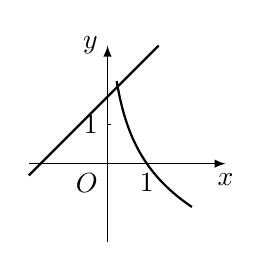
\begin{tikzpicture}[scale = 0.5,>=latex]
    \draw [->] (-2,0) -- (3,0) node [below] {$x$};
    \draw [->] (0,-2) -- (0,3) node [left] {$y$};
    \draw (0,0) node [below left] {$O$};
    \draw (0.1,1) -- (0,1) node [left] {$1$};
    \draw (1,0) node [below] {$1$};
    \draw [thick] (-2,-0.3) -- (1.3,3);
    \draw [thick,domain =-1.1:2.1,samples = 200] plot ({0.5^\x},\x);
\end{tikzpicture}
}{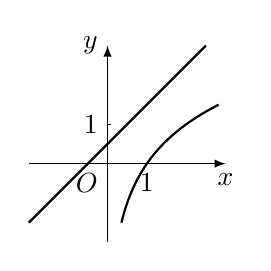
\begin{tikzpicture}[scale = 0.5,>=latex]
    \draw [->] (-2,0) -- (3,0) node [below] {$x$};
    \draw [->] (0,-2) -- (0,3) node [left] {$y$};
    \draw (0,0) node [below left] {$O$};
    \draw (0.1,1) -- (0,1) node [left] {$1$};
    \draw (1,0) node [below] {$1$};
    \draw [thick] (-2,-1.5) -- (2.5,3);
    \draw [thick,domain =1.5:-1.5,samples = 200] plot ({0.5^\x},-\x);
\end{tikzpicture}
}{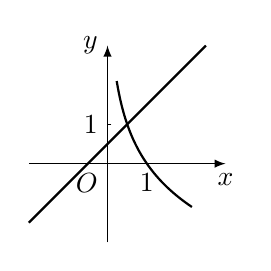
\begin{tikzpicture}[scale = 0.5,>=latex]
    \draw [->] (-2,0) -- (3,0) node [below] {$x$};
    \draw [->] (0,-2) -- (0,3) node [left] {$y$};
    \draw (0,0) node [below left] {$O$};
    \draw (0.1,1) -- (0,1) node [left] {$1$};
    \draw (1,0) node [below] {$1$};
    \draw [thick] (-2,-1.5) -- (2.5,3);
    \draw [thick,domain =-1.1:2.1,samples = 200] plot ({0.5^\x},\x);
\end{tikzpicture}
}{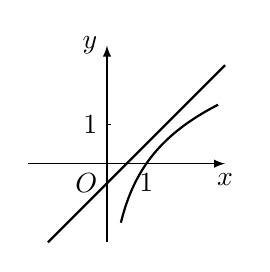
\begin{tikzpicture}[scale = 0.5,>=latex]
    \draw [->] (-2,0) -- (3,0) node [below] {$x$};
    \draw [->] (0,-2) -- (0,3) node [left] {$y$};
    \draw (0,0) node [below left] {$O$};
    \draw (0.1,1) -- (0,1) node [left] {$1$};
    \draw (1,0) node [below] {$1$};
    \draw [thick] (-1.5,-2) -- (3,2.5);
    \draw [thick,domain =1.5:-1.5,samples = 200] plot ({0.5^\x},-\x);
\end{tikzpicture}
}
\item {\tiny (000063)}求下列函数的的定义域:\\
(1) $y=(x-1)^{\frac 52}$;\\
(2) $y=3^{\sqrt{x-1}}$;\\
(3) $y=\lg \dfrac{1+x}{1-x}$.
\item {\tiny (000065)}设点$(\sqrt 2, 2)$在幂函数$y_1=x^a$的图像上, 点$(-2,\dfrac 14)$在幂函数$y_2=x^b$的图像上. 当$x$取何值时, $y_1=y_2$?
\item {\tiny (000070)}选择题:\\
(1) 若$m>n>1$, 而$0<x<1$, 则下列不等式正确的是\bracket{20}.
\fourch{$m^x<n^x$}{$x^m<x^n$}{$\log_x m>\log_x n$}{$\log_m x<\log_n x$}
(2) 在同一平面直角坐标系中, 二次函数$y=ax^2+bx$与指数函数$y=(\dfrac ba)^x$的图像关系可能为\bracket{20}.
\fourch{
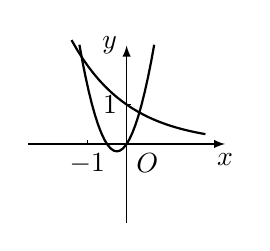
\begin{tikzpicture}[scale = 0.5, >=latex]
    \draw [->] (-2.5,0) -- (2.5,0) node [below] {$x$};
    \draw [->] (0,-2.) -- (0,2.5) node [left] {$y$};
    \draw (0,0) node [below right] {$O$};
    \draw (-1,0.1) -- (-1,0) node [below] {$-1$};
    \draw (0.1,1) -- (0,1) node [left] {$1$};
    \draw [domain = -1.2:0.7,thick] plot (\x,{3*\x * (\x+0.5)});
    \draw [domain = -1.4:2,thick] plot (\x,{(0.5)^\x}); 
\end{tikzpicture}
}{
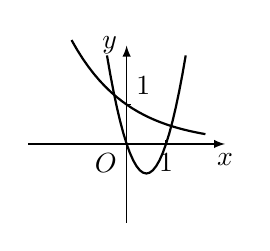
\begin{tikzpicture}[scale = 0.5, >=latex]
    \draw [->] (-2.5,0) -- (2.5,0) node [below] {$x$};
    \draw [->] (0,-2.) -- (0,2.5) node [left] {$y$};
    \draw (0,0) node [below left] {$O$};
    \draw (1,0.1) -- (1,0) node [below] {$1$};
    \draw (0.1,1) -- (0,1) node [above right] {$1$};
    \draw [domain = -0.5:1.5,thick] plot (\x,{3*\x*(\x-1)});
    \draw [domain = -1.4:2,thick] plot (\x,{(0.5)^\x}); 
\end{tikzpicture}
}{
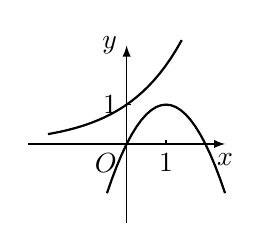
\begin{tikzpicture}[scale = 0.5, >=latex]
    \draw [->] (-2.5,0) -- (2.5,0) node [below] {$x$};
    \draw [->] (0,-2.) -- (0,2.5) node [left] {$y$};
    \draw (0,0) node [below left] {$O$};
    \draw (1,0.1) -- (1,0) node [below] {$1$};
    \draw (0.1,1) -- (0,1) node [left] {$1$};
    \draw [domain = -0.5:2.5,thick] plot ({\x},{-\x*(\x-2)});
    \draw [domain = -1.4:2,thick] plot ({-\x},{(0.5)^\x}); 
\end{tikzpicture}
}{
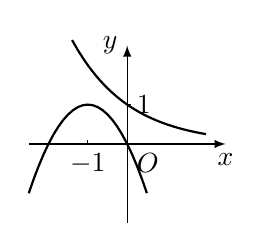
\begin{tikzpicture}[scale = 0.5, >=latex]
    \draw [->] (-2.5,0) -- (2.5,0) node [below] {$x$};
    \draw [->] (0,-2.) -- (0,2.5) node [left] {$y$};
    \draw (0,0) node [below right] {$O$};
    \draw (-1,0.1) -- (-1,0) node [below] {$-1$};
    \draw (0.1,1) -- (0,1) node [right] {$1$};
    \draw [domain = -2.5:0.5,thick] plot ({\x},{-\x*(\x+2)});
    \draw [domain = -1.4:2,thick] plot ({\x},{(0.5)^\x}); 
\end{tikzpicture}   
}
\item {\tiny (000072)}在同一平面直角坐标系中, 作出函数$y=(\dfrac 12)^x$及$y=x^{\frac 12}$的大致图像, 并求方程$(\dfrac 12)^x=x^{\frac 12}$的解的个数.
\item {\tiny (000076)}求函数$y=\dfrac1{2-x}+\sqrt{x^2-1}$的定义域.
\item {\tiny (000080)}分别作出下列函数的大致图像, 并指出它们的单调区间:\\
(1) $y=|x^2-4x|$;\\
(2) $y=2|x|-3$.
\item {\tiny (000083)}邮局规定: 当邮件质量不超过$100$g时, 每$20$g邮费$0.8$元, 且不足$20$g时按$20$g计算; 超过$100$g时, 超过$100$g的部分按每$100$g邮费$2$元计算, 且不足$100$g按$100$g
计算; 同时规定邮件总质量不得超过$2000$g. 请写出邮费关于邮件质量的函数表达式, 并计算$50$g和$500$g的邮件分别收多少邮费.
\item {\tiny (000084)}若函数$y=(a^2+4a-5)x^2-4(a-1)x+3$的图像都在$x$轴上方(不含$x$轴), 求实数$a$的取值范围.
\item {\tiny (000085)}已知$y=f(x)$是奇函数, 其定义域为$\mathbf{R}$; 而$y=g(x)$是偶函数, 其定义域为$D$. 判断函数$y=f(x)g(x)$的奇偶性, 并说明理由.
\item {\tiny (000092)}作出函数$y=(x^2-1)^2-1$的大致图像, 写出它的单调区间, 并证明你的结论.
\item {\tiny (000094)}设函数$y=f(x)$, $x\in \mathbf{R}$的反函数是$y=f^{-1}(x)$.\\
(1) 如果$y=f(x)$是奇函数, 那么$y=f^{-1}(x)$的奇偶性如何?\\
(2) 如果$y=f(x)$在定义域上是严格增函数, 那么$y=f^{-1}(x)$的单调性如何?
\item {\tiny (000330)}若函数$f(x)=\log_2\dfrac{x-a}{x+1}$的反函数的图像过点$(-2,3)$, 则$a=$\blank{50}.
\item {\tiny (000342)}若函数$f(x)=\begin{cases}    2^x, & x\le 0, \\ -x^2+m, & x>0 \end{cases}$的值域为$(-\infty ,1]$, 则实数$m$的取值范围是\blank{50}.
\item {\tiny (000349)}若函数$f(x)=\log_2 (x+1)+a$的反函数的图像经过点$(4,1)$, 则实数$a=$\blank{50}.
\item {\tiny (000355)}有以下命题:\\
\textcircled{1} 若函数$f(x)$既是奇函数又是偶函数, 则$f(x)$的值域为$\{0\}$; \\
\textcircled{2} 若函数$f(x)$是偶函数, 则$f(|x|)=f(x)$;\\
\textcircled{3} 若函数$f(x)$在其定义域内不是单调函数, 则$f(x)$不存在反函数;\\
\textcircled{4} 若函数$f(x)$存在反函数${{f}^{-1}}(x)$, 且${{f}^{-1}}(x)$与$f(x)$不完全相同, 则$f(x)$与${{f}^{-1}}(x)$图像的公共点必在直线$y=x$上; \\
其中真命题的序号是\blank{50}(写出所有真命题的序号).
\item {\tiny (000381)}若点$(8,4)$在函数$f(x)=1+\log_a x$图像上, 则$f(x)$的反函数为\blank{50}.
\item {\tiny (000388)}已知函数$f(x)=a^x-1$的图像经过$(1,1)$点, 则$f^{-1}(3)=$\blank{50}.
\item {\tiny (000450)}函数$f(x)=2^x+m$的反函数为$y=f^{-1}(x)$, 且$y=f^{-1}(x)$的图像过点$Q(5,2)$, 那么$m=$\blank{50}.
\item {\tiny (000472)}若函数$f(x)=x^a$的反函数的图像经过点$(\dfrac12,\dfrac14)$, 则$a=$\blank{50}.
\item {\tiny (000486)}函数$f(x)=\lg(2-x)$的定义域是\blank{50}.
\item {\tiny (000498)}已知幂函数的图像过点$(2,\dfrac14)$, 则该幂函数的单调递增区间是\blank{50}.
\item {\tiny (000520)}已知函数$f(x)=a\cdot 2^x+3-a\ (a\in \mathbf{R})$的反函数为$y=f^{-1}(x)$, 则函数$y=f^{-1}(x)$的图像经过的定点的坐标为\blank{50}.
\item {\tiny (000567)}函数$f(x)=\sqrt{1-\lg x}$的定义域为\blank{50}.
\item {\tiny (000582)}数列$\{a_n\}$的前$n$项和为$S_n$, 若点$(n,S_n) \ (n\in \mathbf{N}^*)$在函数$y=\log_2 (x+1)$的反函数的图像上, 则$a_n$=\blank{50}.
\item {\tiny (000590)}已知函数$f(x)=1+\log_a x$, $y=f^{-1}(x)$是函数$y=f(x)$的反函数, 若$y=f^{-1}(x)$的图像过点$(2,4)$, 则$a$的值为\blank{50}.
\item {\tiny (000607)}函数$y=\log_2(1-\dfrac1x)$的定义域为\blank{50}.
\item {\tiny (000634)}若函数$f(x)=4^x+2^{x+1}$的图像与函数$y=g(x)$的图像关于直线$y=x$对称, 则$g(3)=$\blank{50}.
\item {\tiny (000646)}函数$y=\sqrt{2x-x^2}$的定义域是\blank{50}.
\item {\tiny (000655)}若将函数$f(x)=|\sin(\omega x-\dfrac{\pi}8)| \ (\omega >0)$的图像向左平移$\dfrac{\pi}{12}$个单位后, 所得图像对应的函数为偶函数, 则$\omega$的最小值是\blank{50}.
\item {\tiny (000675)}已知定义在$\mathbf{R}$上的函数$f(x)$满足: \textcircled{1} $f(x)+f(2-x)=0$; \textcircled{2} $f(x)-f(-2-x)=0$; \textcircled{3} 在$[-1,1]$上的表达式为$f(x)=\begin{cases} \sqrt{1-x^2}, & x\in [-1,0], \\ 1-x, & x\in (0,1] \end{cases}$, 则函数$f(x)$与函数$g(x)=\begin{cases} 2^x, & x\le 0, \\ \log_{\frac12} x,& x>0 \end{cases}$的图像在区间$[-3,3]$上的交点的个数为\blank{50}.
\item {\tiny (000715)}设奇函数$f(x)$的定义域为$\mathbf{R}$, 当$x>0$时,$f(x)=x+\dfrac{m^2}x-1$(这里$m$为正常数). 若$f(x)\le m-2$对一切$x\le 0$成立, 则$m$的取值范围为\blank{50}.
\item {\tiny (000758)}若函数$f(x)=\sqrt{8-ax-2x^2}$是偶函数, 则该函数的定义域是\blank{50}.
\item {\tiny (000778)}函数$y=\sqrt{\lg(x+2)}$的定义域为\blank{50}.
\item {\tiny (000845)}已知函数$f(x)=\lg (\sqrt{x^2+1}+ax)$的定义域为$\mathbf{R}$, 则实数$a$的取值范围是\blank{50}.
\item {\tiny (000851)}已知函数$f(x)=\dfrac{3x+1}{x+a}\ (a\ne \dfrac13)$的图像与它的反函数的图像重合, 则实数$a$的值为\blank{50}.
\item {\tiny (000859)}设$a>0$且$a\ne 1$, 若函数$f(x)=a^{x-1}+2$的反函数的图像经过定点$P$, 则点$P$的坐标是\blank{50}.
\item {\tiny (000868)}函数$f(x)=\dfrac{\sqrt{x+2}}{x-1}$的定义域为\blank{50}.
\item {\tiny (000931)}函数$y=\log_3 (x-1)$的定义域是\blank{50}.
\item {\tiny (000949)}已知函数$f(x)={x^3}+\lg (\sqrt{x^2+1}+x)$, 若$f(x)$的定义域中的$a$、$b$满足$f(-a)+f(-b)-3=f(a)+f(b)+3$, 则$f(a)+f(b)=$\blank{50}.
\item {\tiny (000961)}已知函数$f(x)=2^x-a\cdot 2^{-x}$的反函数是$f^{-1}(x)$, $f^{-1}(x)$在定义域上是奇函数, 则正实数$a=$\blank{50}.
\item {\tiny (001160)}已知函数$f(x)=3x+5, \ x\in \mathbf{R}$, 求$f(-1)$, $f(10)$, $f(a)$, $f(a^2+1)$. 并写出函数$y=f(f(x))$的定义域, 对应法则以及值域.
\item {\tiny (001164)}写出下列函数的定义域(写在对应关系的右边):\\ 
(1) $f(x)=\dfrac{6}{x^2-3x+2}$;\\ 
(2) $f(x)=\dfrac{3x-1}{2x^3+4x^2+x-7}$;\\ 
(3) $f(x)=\dfrac{\sqrt[3]{4x+8}}{\sqrt{3x-2}}$;\\ 
(4) $f(x)=\sqrt{2x-1}+\sqrt{1-2x}+4$;\\ 
(5) $f(x)=\sqrt{x^2-4}$;\\ 
(6) $f(x)=\dfrac{\sqrt{2x+1}}{x-3}$.
\item {\tiny (001165)}(1) 函数$f(x)=x^2, \ x \in [0,1]$的值域为\blank{50};\\ 
(2) 函数$f(x)=-x, \ x \in [-1,0)$的值域为\blank{50};\\ 
(3) 函数$f(x)=\left\{\begin{array}{cc}x^2,&0\le x\le 1,\\-x,&-1\le x<0.\end{array}\right.$的值域为\blank{50}.
\item {\tiny (001166)}函数$f(x)=\sqrt{kx^2+4kx+3}$的定义域为$\mathbf{R}$, 求实数$k$的取值范围.
\item {\tiny (001167)}求函数$y=x^3+1$的值域(要详细过程).
\item {\tiny (001173)}在以下坐标系中分别作出下列函数的图像(用铅笔, 要求清晰, 交代关键信息):\\ 
\begin{tabular}{ll}
(1) $y=\sqrt{|x|}$;& (2) $y=|x-1|-|x+1|$;\\
\begin{tikzpicture}[>=latex]
    \foreach \i in {-4,-3,...,4} {\draw [dashed, gray!90] (-4,\i) -- (4,\i) (\i,-4) -- (\i,4);};
    \draw [->] (-4,0) -- (4,0) node [below] {$x$};
    \draw [->] (0,-4) -- (0,4) node [left] {$y$};
    \draw (0,0) node [below left] {$O$};
    \draw (0,1) node [left] {$1$};
    \draw (1,0) node [below] {$1$};
\end{tikzpicture} & 
\begin{tikzpicture}[>=latex]
    \foreach \i in {-4,-3,...,4} {\draw [dashed, gray!90] (-4,\i) -- (4,\i) (\i,-4) -- (\i,4);};
    \draw [->] (-4,0) -- (4,0) node [below] {$x$};
    \draw [->] (0,-4) -- (0,4) node [left] {$y$};
    \draw (0,0) node [below left] {$O$};
    \draw (0,1) node [left] {$1$};
    \draw (1,0) node [below] {$1$};
\end{tikzpicture}
\end{tabular}
\begin{tabular}{ll}
(3) $y=x-[x]$;& (4) $y=x+\dfrac{1}{x}$;\\
\begin{tikzpicture}[>=latex]
    \foreach \i in {-4,-3,...,4} {\draw [dashed, gray!90] (-4,\i) -- (4,\i) (\i,-4) -- (\i,4);};
    \draw [->] (-4,0) -- (4,0) node [below] {$x$};
    \draw [->] (0,-4) -- (0,4) node [left] {$y$};
    \draw (0,0) node [below left] {$O$};
    \draw (0,1) node [left] {$1$};
    \draw (1,0) node [below] {$1$};
\end{tikzpicture} & 
\begin{tikzpicture}[>=latex]
    \foreach \i in {-4,-3,...,4} {\draw [dashed, gray!90] (-4,\i) -- (4,\i) (\i,-4) -- (\i,4);};
    \draw [->] (-4,0) -- (4,0) node [below] {$x$};
    \draw [->] (0,-4) -- (0,4) node [left] {$y$};
    \draw (0,0) node [below left] {$O$};
    \draw (0,1) node [left] {$1$};
    \draw (1,0) node [below] {$1$};
\end{tikzpicture}
\end{tabular}
\begin{tabular}{ll}
(5) $y=x-\dfrac{1}{x}$;& (6) $y=\dfrac{6x}{1+x^2}$.\\
\begin{tikzpicture}[>=latex]
    \foreach \i in {-4,-3,...,4} {\draw [dashed, gray!90] (-4,\i) -- (4,\i) (\i,-4) -- (\i,4);};
    \draw [->] (-4,0) -- (4,0) node [below] {$x$};
    \draw [->] (0,-4) -- (0,4) node [left] {$y$};
    \draw (0,0) node [below left] {$O$};
    \draw (0,1) node [left] {$1$};
    \draw (1,0) node [below] {$1$};
\end{tikzpicture} & 
\begin{tikzpicture}[>=latex]
    \foreach \i in {-4,-3,...,4} {\draw [dashed, gray!90] (-4,\i) -- (4,\i) (\i,-4) -- (\i,4);};
    \draw [->] (-4,0) -- (4,0) node [below] {$x$};
    \draw [->] (0,-4) -- (0,4) node [left] {$y$};
    \draw (0,0) node [below left] {$O$};
    \draw (0,1) node [left] {$1$};
    \draw (1,0) node [below] {$1$};
\end{tikzpicture}
\end{tabular}
\item {\tiny (001174)}某种茶杯每个$0.5$元, 买$x$个茶杯的钱数为$y$元. 画出$y$关于$x$的函数的图像.\\ 
\begin{tikzpicture}[>=latex]
    \foreach \i in {0,1,...,7} {\draw [dashed, gray!90] (0,\i) -- (16,\i);};
    \foreach \i in {0,1,...,16} {\draw [dashed, gray!90] (\i,0) -- (\i,7);};
    \draw [->] (-0.5,0) -- (16,0) node [below] {$x$};
    \draw [->] (0,-0.5) -- (0,7) node [left] {$y$};
    \draw (0,0) node [below left] {$O$};
    \draw (0,1) node [left] {$1$};
    \draw (1,0) node [below] {$1$};
\end{tikzpicture}
\item {\tiny (001175)}证明: 函数$y=\dfrac{1}{x}$的图像关于原点对称(一个图形关于原点对称是指任取该图形上的一点, 它关于原点对称所得的点也在该图形上).
\item {\tiny (001176)}求证: 函数$y=x^3$的图像不是一条直线(本题不能使用斜率的概念).
\item {\tiny (001177)}试求出函数$y=x^2$的图像分别进行如下变换后, 所得的各个图像对应的函数.\\ 
(1) 向右平移$2$个单位;\\ 
(2) 向上平移$1$个单位;\\ 
(3) 先向右平移$2$个单位, 再向上平移$1$个单位;\\ 
(4) 先向上平移$1$个单位, 再向右平移$2$个单位
\item {\tiny (001178)}试求出函数$y=\sqrt{x}$的图像分别进行如下变换后所得的各个图像对应的函数.\\ 
(1) 图像上的每一点的横坐标变为原来的$2$倍;\\ 
(2) 图像上的每一点的纵坐标变为原来的$\dfrac{1}{2}$;\\ 
(3) 图像上的每一点的横坐标变为原来的$2$倍, 然后向上平移$3$个单位, 所得图像上每一点的纵坐标变为原来的$3$倍, 再向左平移$2$个单位;\\ 
(4) 向左平移$3$个单位, 然后将所得图像上的每一点的横坐标变为原来的$\dfrac{1}{2}$, 最后向下平移$2$个单位
\item {\tiny (001179)}欲将函数$y=3x$的图像通过一次平移变为函数$y=3x-5$的图像, 可向\blank{50}平移\blank{50}个单位; 也可向\blank{50}平移\blank{50}个单位.
\item {\tiny (001180)}欲将函数$y=x^2$的图像通过平移和放缩变为函数$y=2x^2-4x-1$的图像, 所需的步骤依次为: (同时写出每步变换后所得图像对应的函数)
\item {\tiny (001181)}证明: 在平面直角坐标系中, 将函数$y=f(x),x\in \mathbf{R}$的图像绕原点旋转$180^\circ$, 得到的是函数$y=-f(-x),x\in \mathbf{R}$的图像.
\item {\tiny (001182)}在平面直角坐标系中, 将函数$y=f(x),x\in \mathbf{R}$的图像沿直线$x=1$翻折, 将会得到哪个函数的图像? 试写出这个函数, 并证明.
\item {\tiny (001185)}已知$f(x)=x^2$, $g(x)=\dfrac{1}{x}$.\\ 
(1) 求$f(x)+g(x)$, $f(x)g(x)$和$\dfrac{f(x)}{g(x)}$;\\ 
(2) 求$f\circ g$和$g\circ f$;\\ 
(3) 求$f\circ g-g\circ f$, 判断它是否在其定义域上恒等于零.
\item {\tiny (001186)}已知$f(x)=x^2$, $g(x)=\dfrac{1}{x+1}$.\\ 
(1) 求$f(x)+g(x)$, $f(x)g(x)$和$\dfrac{f(x)}{g(x)}$;\\ 
(2) 求$f\circ g$和$g\circ f$;\\ 
(3) 求$f\circ g-g\circ f$, 判断它是否在其定义域上恒等于零.
\item {\tiny (001190)}下列各映射中, 是单射的有\blank{60}, 是满射的有\blank{60}, 存在逆映射的有\blank{60}.\\ 
\textcircled{1} $f: \{1,2,3\}\rightarrow \{1,4,9\}; \ x\mapsto x^2$;\\ 
\textcircled{2} $f: \mathbf{R}^+\rightarrow \mathbf{R}^+; \ x \mapsto x^2$;\\ 
\textcircled{3} $f: \mathbf{R}\rightarrow [0,+\infty); \ x \mapsto x^2$;\\ 
\textcircled{4} $f: \mathbf{R}^+\rightarrow \mathbf{R}^+; \ x \mapsto \dfrac{1}{x}$;\\ 
\textcircled{5} $f: \mathbf{R}^+\cup \mathbf{R}^-\rightarrow \mathbf{R}^+\cup \mathbf{R}^-; \ x \mapsto \dfrac{1}{x}$;\\ 
\textcircled{6} $f: \mathbf{R}^+\rightarrow \mathbf{R}; \ x \mapsto x+\dfrac{1}{x}$;\\ 
\textcircled{7} $f: \mathbf{R}^+\rightarrow \mathbf{R}; \ x \mapsto x-\dfrac{1}{x}$;\\ 
\textcircled{8} $f: \mathbf{R}\rightarrow \mathbf{Z}; \ x \mapsto [x]$;\\ 
\textcircled{9} $f: \{(x,y)|x,y\in \mathbf{R}\}\rightarrow \{(x,y)|x,y\in \mathbf{R}\};\ (x,y)\mapsto (x+y,x-y)$;\\ 
\textcircled{10} $f: \{(x,y)|x,y\in \mathbf{R}\}\rightarrow \{(x,y)|x,y\in \mathbf{R}\};\ (x,y)\mapsto (x+y,2x+2y)$.
\item {\tiny (001192)}写出下列函数的反函数(注意定义域).\\ 
(1) $y=-\dfrac{1}{x}+3$;\\ 
(2) $y=\sqrt{2x-1}$;\\ 
(3) $y=\dfrac{2x+1}{x+2}$;\\ 
(4) $y=x^2+2, \ x\in [2,+\infty)$;\\ 
(5) $y=2^x, \ x\in \{1,2,3,4\}$ (本小题不能使用对数);\\ 
(6) $y=\sqrt{9-x^2}, \ x\in [-3,0]$;\\ 
(7) $y=x^2-4x, x \in [3,7]$.
\item {\tiny (001193)}已知函数$y=f(x)$的图像经过$(1,2)$, 它有反函数$y=f^{-1}(x)$. 那么函数$y=f^{-1}(x+3)$的图像一定经过点\blank{50}.
\item {\tiny (001194)}已知函数$y=f(x)$有反函数, 且$y=f^{-1}(3x+1)$的图像经过点$(0,-1)$. 试确定函数$y=5f(x+2)+3$的图像一定经过的点, 并说明理由.
\item {\tiny (001196)}已知函数$y=f(x)$的图像经过第一, 第二象限, 且它有反函数$y=f^{-1}(x)$. 那么$y=f^{-1}(x)$的图像一定经过\blank{80}象限.
\item {\tiny (001198)}在同一坐标系中通过平移和放缩作出以下函数的图像, 并写出变换的方法.
$y=|x|$; $y=|x-1|$; $y=\dfrac{|x-1|}2$; $y=\dfrac{|x-1|}2-3$; $y=\dfrac{|2x-1|}2-3$.
\begin{center}
\begin{tikzpicture}[>=latex]
    \foreach \i in {-4,-3,...,4} {\draw [dashed, gray!90] (-4,\i) -- (4,\i) (\i,-4) -- (\i,4);};
    \draw [->] (-4,0) -- (4,0) node [below] {$x$};
    \draw [->] (0,-4) -- (0,4) node [left] {$y$};
    \draw (0,0) node [below left] {$O$};
    \draw (0,1) node [left] {$1$};
    \draw (1,0) node [below] {$1$};
\end{tikzpicture}
\end{center}
\item {\tiny (001199)}(1)欲将函数$y=x^2$的图像通过先平移后放缩的方式变为函数$y=\dfrac{1}{2}x^2+x$的图像, 所需的步骤依次为: (同时写出每步变换后所得图像对应的函数)\\ 
(2)欲将函数$y=x^2$的图像通过先放缩后平移的方式变为函数$y=\dfrac{1}{2}x^2+x$的图像, 所需的步骤依次为: (同时写出每步变换后所得图像对应的函数)
\item {\tiny (001200)}(1)欲将函数$y=\sqrt{x}$的图像通过先平移后放缩的方式变为函数$y=\sqrt{2x-4}$的图像, 所需的步骤依次为: (同时写出每步变换后所得图像对应的函数)\\ 
(2)欲将函数$y=\sqrt{x}$的图像通过先放缩后平移的方式变为函数$y=\sqrt{2x-4}$的图像, 所需的步骤依次为: (同时写出每步变换后所得图像对应的函数)
\item {\tiny (001201)}将函数$y=\sqrt{x}$的图像上的每一点的横坐标变为原来的$3$倍, 然后向右平移$3$个单位, 再沿直线$y=x$翻折, 则所得图像对应的函数为\blank{50}.
\item {\tiny (001202)}[选做]
欲将函数$y=|x-1|+|x+1|$的图像通过平移和放缩变为函数$y=|x-2|+|x-6|$的图像, 所需的步骤依次为: (同时写出每步变换后所得图像对应的函数, 提示: 先把两个函数的图像画在一张草稿纸上找一下感觉)
\item {\tiny (001203)}[选做]
欲将函数$y=x+\dfrac{1}{x}$的图像通过放缩变为函数$y=x+\dfrac{4}{x}$的图像, 所需的步骤依次为: (同时写出每步变换后所得图像对应的函数, 提示: 先把两个函数的图像画在一张草稿纸上找一下感觉)
\item {\tiny (001204)}奇函数的图像是否都过原点? 偶函数的图像是否一定和$y$轴相交? 为什么?
\item {\tiny (001207)}已知$y=f(x)$, $y=g(x)$的定义域均关于原点对称且交集非空, 且$f$与$g$一奇一偶, 证明: $y=f(x)g(x)$是奇函数.
\item {\tiny (001213)}已知函数$y=f(x)$与$y=g(x)$的定义域均为$\mathbf{R}$.\\ 
\blank{25}(1) 如果$y=f(x)$是奇函数, 那么$y=|f(x)|$是偶函数;\\ 
\blank{25}(2) 如果$y=f(x)$是奇函数, 那么$y=\sqrt[3]{f(x)}$是奇函数;\\ 
\blank{25}(3) 如果$y=f(x)$是奇函数, 那么$y=f(|x|)$是奇函数;\\ 
\blank{25}(4) 如果$y=f(x)$是奇函数, 那么$y=f(|x|)$是偶函数;\\ 
\blank{25}(5) 如果$y=f(x)$是奇函数, $y=g(x)$是偶函数, 那么$y=f(x)g(x)$是奇函数;\\ 
\blank{25}(6) 如果$y=f(x)$是奇函数, $y=g(x)$不是偶函数, 那么$y=f(x)+2g(x)$既非奇函数又非偶函数;\\ 
\blank{25}(7) 如果$y=f(x)$不是奇函数, $y=g(x)$也不是奇函数, 那么$y=f(x)-g(x)$也不是奇函数;\\ 
\blank{25}(8) 如果$y=f(x)$是奇函数, $y=g(x)$不是偶函数, 那么$y=f(x)+g(x)$不是偶函数;\\ 
\blank{25}(9) 如果$y=f(x)-g(x)$是奇函数, $y=g(x)$是奇函数, 那么$y=f(x)$也是奇函数;\\ 
\blank{25}(10) 如果$y=(f(x))^2$是偶函数, 那么$y=f(x)$是偶函数或者是奇函数;\\ 
\blank{25}(11) 如果$y=(f(x))^2$是奇函数, 那么$y=f(x)$恒等于零, 因此是奇函数也是偶函数;\\ 
\blank{25}(12) 如果$y=(f(x))^3$是奇函数, 那么$y=f(x)$是奇函数.
\item {\tiny (001214)}已知函数$y=f(x),\ x \in D_f$与$y=g(x),\ x \in D_g$的定义域交集非空.\\ 
\blank{25}(1) 如果$y=f(x)$是奇函数, $y=g(x)$是奇函数, 那么$y=f(x)+x^2g(x)$是奇函数;\\ 
\blank{25}(2) 如果$y=f(x)$是奇函数, $y=g(x)$是偶函数, 而且它们都不恒等于零, 那么$y=f(x)+g(x)$既不是奇函数又不是偶函数;\\ 
\blank{25}(3) 如果$y=f(x)$是奇函数, $y=g(x)$是偶函数, 而且它们在$D_f\cap D_g$上都不恒等于零, 那么$y=f(x)+g(x)$既不是奇函数又不是偶函数;\\ 
\blank{25}(4) 如果$y=f(x)$不是奇函数, $y=g(x)$也不是奇函数, 那么$y=f(x)-g(x)$也不是奇函数;\\ 
\blank{25}(5) 如果$y=|f(x)|$是奇函数, 那么$f(x)$恒等于零;\\ 
\blank{25}(6) 如果$y=f(x)$不是奇函数, 那么$y=|f(x)|$不是偶函数;\\ 
\blank{25}(7) 如果$y=f(x)$是偶函数, 且$y=f(x)+g(x)$也是偶函数, 那么$y=g(x)$也是偶函数.
\item {\tiny (001215)}已知$y=f(x), \ x \in D$是偶函数.\\ 
\blank{25}(1) $y=(f(x))^3+f(x)$是偶函数;\\ 
\blank{25}(2) $y=f(2x)$是偶函数;\\ 
\blank{25}(3) $y=f(x-1)$的图像关于直线$x=-1$对称;\\ 
\blank{25}(4) $y=f(x-1)$的图像关于直线$x=1$对称;\\ 
\blank{25}(5) $y=f(3x+1)$的图像关于直线$x=-\dfrac{1}{3}$对称;\\ 
\blank{25}(6) $y=f(3x+1)$的图像关于直线$x=-1$对称;\\ 
\blank{25}(7) $y=f(x^3+1)$是偶函数;\\ 
\blank{25}(8) $y=f(x^3+x)$是偶函数.
\item {\tiny (001216)}已知$y=f(x)$是奇函数.\\ 
\blank{25}(1) $y=f(3x)$是奇函数;\\ 
\blank{25}(2) $y=f(x-1)+2$的图像关于点$(1,2)$对称;\\ 
\blank{25}(3) $y=3f(2x-1)+6$的图像关于点$(1,6)$对称;\\ 
\blank{25}(4) $y=3f(2x-1)+6$的图像关于点$(\dfrac{1}{2},6)$对称;\\ 
\blank{25}(5) $y=3f(2x-1)+6$的图像关于点$(\dfrac{1}{2},2)$对称;\\ 
\blank{25}(6) $y=f(x^2)$是偶函数;\\ 
\blank{25}(7) $y=f^{-1}(x)$一定存在;\\ 
\blank{25}(8) $y=f^{-1}(x)$如果存在, 则必定是奇函数.
\item {\tiny (001231)}已知函数$y=\dfrac{1}{2}x^2-x+\dfrac{3}{2}$的定义域为$[1,b]$, 最大值为$b$, 最小值为$1$. 求$b$.
\item {\tiny (001232)}已知函数$f(x)=\dfrac{x^2+2x+a}{x}, \ x \in [1,+\infty)$.\\ 
(1) 当$a=4$时, 求函数的最小值;\\ 
(2) 如果对一切定义域中的$x$, $f(x)$均为正数, 求实数$a$的取值范围.
\item {\tiny (001237)}证明: 函数$y=x^3+x,x\in [1,2]$的值域为$[2,10]$
\item {\tiny (001238)}函数$y=x^2-3x+1, \ x \in [1,4]$的值域为\blank{80}.
\item {\tiny (001239)}函数$y=\dfrac{2x+3}{x-1}$的值域为\blank{80}.
\item {\tiny (001240)}函数$y=\dfrac{6x}{x^2+1}$的值域为\blank{80}.
\item {\tiny (001241)}函数$y=x^5+3x+1, \ x \in [1,3]$的值域为\blank{80}.
\item {\tiny (001242)}函数$y=\sqrt{1+x}+2x$的值域为\blank{80}.
\item {\tiny (001243)}函数$y=|x-3|-|x-10|$的值域为\blank{80}.
\item {\tiny (001244)}函数$y=|x-3|+|x-10|+|x+1|+|x+2|$的值域为\blank{80}.
\item {\tiny (001245)}函数$y=||x-3|+x|$的值域为\blank{80}.
\item {\tiny (001246)}求函数$y=\dfrac{x^2-4x+5}{x^2-x-1}$的值域.
\item {\tiny (001247)}已知函数$y=\sqrt{x}+\sqrt{x+a}$的值域为$[\dfrac{\sqrt{3}}{2},+\infty)$, 求实数$a$.
\item {\tiny (001248)}求函数$y=|x-1|+|x-2|+|x-3|+\cdots+|x-20|$的值域.
\item {\tiny (001249)}求函数$y=|x-1|+|x-2|+|x-3|+\cdots+|x-50|+|100x-400|$的值域(提示, 某种程度上来说这题目反而比上一题简单).
\item {\tiny (001250)}函数$y=\sqrt{1+\sqrt{1+\sqrt{1+\sqrt{x^2+64}}}}$的值域为\blank{80}.
\item {\tiny (001251)}函数$y=\dfrac{1}{1+\frac{1}{x}}$的值域为\blank{80}.
\item {\tiny (001252)}函数$y=\dfrac{1}{x^2+x+1}$的值域为\blank{80}.
\item {\tiny (001253)}函数$y=\dfrac{x^2}{x^2+x+1}$的值域为\blank{80}.
\item {\tiny (001254)}函数$y=4-\sqrt{4-x^2}$的值域为\blank{80}.
\item {\tiny (001255)}函数$y=\dfrac{\sqrt{x}}{1+x}$的值域为\blank{80}.
\item {\tiny (001256)}函数$y=\sqrt{6-x}+\sqrt{x-3}$的值域为\blank{80}.
\item {\tiny (001257)}函数$y=\dfrac{6x}{x^2+1}, \ x \in [-\dfrac{1}{2},5]$的值域为\blank{80}.
\item {\tiny (001258)}求函数$y=\dfrac{2x^2+3x+1}{x-1}(x\in(1,+\infty))$的值域.
\item {\tiny (001259)}求函数$y=\dfrac{2x^2+2x+3}{x^2+x+1}(x\in(-1,+\infty))$的值域.
\item {\tiny (001260)}求函数$y=\dfrac{2x^2+3x+3}{x^2+x+1}(x\in(-1,+\infty))$的值域.
\item {\tiny (001261)}设$a$为实常数, 求函数$y=|x-|x+|x+1|+2|+a|+|10x-10|$的值域. (提示: 不觉得$10x$的系数有点突兀吗?)
\item {\tiny (001262)}已知函数$y=f(2x-1)$的定义域为$[0,3]$, 则函数$y=f(3x+1)$的定义域为\blank{50}.
\item {\tiny (001264)}已知函数$f(x)=\dfrac{a-x}{x-a-1}$的反函数$f^{-1}(x)$的图像关于点$(-1,3)$对称, 则$a=$\blank{50}.
\item {\tiny (001266)}写出下列函数的值域.\\ 
(1) $y=3x+1, \ x \in [-2,5]$; \blank{80}\\ 
(2) $y=|2x+1|, \ x \in [-1,3]$; \blank{80}\\ 
(3) $y=\dfrac{x-1}{2x+3}$; \blank{80}\\ 
(4) $y=\dfrac{|x|+1}{|x|-1}$; \blank{80}\\ 
(5) $y=\dfrac{|x+3|}{x-4}, \ x \in [-4,0]$; \blank{80}\\ 
(6) $y=\dfrac{2x+1}{|x+1|-|x|}$; \blank{80}
\item {\tiny (001267)}(1) 求函数$f(x)=\dfrac{2x-1}{x+1}$的值域;\\ 
(2) 已知$a$是实数, 求函数$f(x)=\dfrac{2x-a}{x+1}$的值域.
\item {\tiny (001271)}写出下列函数的值域:\\ 
(1) $y=x^2+2x+2$; \blank{80}\\ 
(2) $y=-x^2+3x+4$; \blank{80}\\ 
(3) $y=4x^2+x+1, \ x \in [-3,0]$; \blank{80}\\ 
(4) 已知$a>0$, $y=ax^2+ax+2a, \ x \in [-1,1)$; \blank{80}\\ 
(5) $y=\dfrac{1}{x^2+2x+2}$; \blank{80}\\ 
(6) $y=4-\sqrt{4x-4x^2}$; \blank{80}\\ 
(7) $y=\dfrac{x^2-x-2}{x^2+3x+2}$; \blank{80}\\ 
(8) $y=|x^2-2x-3|, \ x \in (\dfrac{1}{2},2]$; \blank{80}
\item {\tiny (001274)}已知$k$是实数, 函数$y=\sqrt{kx^2+2(k+2)x+3(4k-1)}$的定义域为$\mathbf{R}$, 则$k$的取值范围为\blank{50}.
\item {\tiny (001275)}已知$k$是实数, 函数$y=\sqrt{kx^2+2(k+2)x+3(4k-1)}$的值域为$[0,+\infty)$, 则$k$的取值范围为\blank{50}.
\item {\tiny (001281)}已知$a$是实数, 就关于$x$的方程$x^2+(a-5)x+(a-2)=0$的两个根(重根算两个根)的不同分布情况, 利用函数$y=\dfrac{-x^2+5x+2}{x+1}$的图像与性质确定$a$的范围.\\ 
\begin{multicols}{2}
(1) 两个根分别在$(-\infty,2)$和$(2,+\infty)$中;\\ 
(3) 有根在$[0,2)$内;\\ 
(2) 两个根都在$(-\infty,-2)$中;\\ 
(4) 有两个不同的根, 有且仅有一根在$[0,+\infty)$中.\\ 
\end{multicols}
\item {\tiny (001283)}求函数$y=2x+\sqrt{1-x^2}$的值域.
\item {\tiny (001318)}函数$y=\sqrt{3^{2x-1}-27}$的定义域为\blank{80}.
\item {\tiny (001320)}已知$f_1(x)=3^x-1$, $f_2(x)=3^{x-1}$, $f_3(x)=-3^x$, $f_4(x)=-3^{-x}$, $f_5(x)=(1/3)^x$, $f_6(x)=(1/3)^{-x}$. 则将函数$y=3^x$的图像右移$1$单位得\blank{80}的图像, 下移$1$单位得\blank{80}的图像. $y=3^x$的图像与\blank{80}的图像关于$x$轴对称, 与\blank{80}的图像关于$y$轴对称, 与$\blank{80}$的图像关于原点对称, 与\blank{80}的图像完全相同.
\item {\tiny (001322)}写出下列函数的单调区间和值域(不用证明).\\ 
(1) $y=\left(\dfrac{1}{2}\right)^{x^2+2x+3}$;\\ 
(2) $y=\dfrac{1}{3^x-1}$;\\ 
(3) $y=4^x-2^{x+1}$.
\item {\tiny (001327)}函数$y=\sqrt{\log_{\frac{1}{2}}\left(\left(\dfrac{1}{3}\right)^x-27\right)}$的定义域为\blank{80}.
\item {\tiny (001333)}一个函数和它的反函数的图像的公共点是否一定在直线$y=x$上? 为什么?
\item {\tiny (001334)}求证: 若递增函数与其反函数的图像有公共点, 则公共点一定在直线$y=x$上.
\item {\tiny (001335)}已知幂函数的图像过点$(9,\dfrac{\sqrt{3}}{3})$, 则该幂函数为$y=$\blank{50}.
\item {\tiny (001336)}(1) 写出函数$y=x^{-\frac{4}{3}}$的定义域, 奇偶性, 单调区间;\\ 
(2) 写出函数$y=x^{-\frac{3}{4}}$的定义域, 奇偶性, 单调区间.
\item {\tiny (001337)}作出下列函数的大致图像(只要能够表明定义域和单调性, 凹凸性方面的信息):\\ 
\begin{multicols}{2}
(1) $y=x^{\frac{2}{3}}$; \\ 
(2) $y=x^{-\frac{3}{2}}$; \\ 
\end{multicols}
\begin{multicols}{2}
(3) $y=\dfrac{|x|+1}{|x+1|}$;  \\ 
(4) $y=\dfrac{1}{(x-2)^2}-1$.
\end{multicols}
\item {\tiny (001513)}已知$2$是函数$y=f(x),x\in\mathbf{R}$的周期, 且当$x\in(-1,1]$时, $f(x)=1-x^2$.\\ 
(1) 写出该函数的值域以及所有单调增区间;\\ 
(2) 写出方程$f(x)=\dfrac{1}{2}$的解集;\\ 
(3) 当$x\in(99,101]$时,求$f(x)$的解析式.
\item {\tiny (002821)}函数$y=\dfrac{\sqrt{2x+1}}{x-3}+(x-1)^0$的定义域为\blank{50}.
\item {\tiny (002822)}若函数$y=f(x)$的定义域是$[-2,4]$, 则函数$g(x)=f(x)+f(-x)$的定义域是\blank{50}.
\item {\tiny (002827)}已知$y=f(x)$为偶函数, 且$y=f(x)$的图像在$x\in [0,1]$时的部分是半径为$1$的圆弧, 在$x\in [1,+\infty)$时的部分是过点$(2,1)$的射线, 如图.\\
\begin{center}
    \begin{tikzpicture}[>=latex]
        \draw [->] (-1,0) -- (4,0) node [below] {$x$};
        \draw [->] (0,-1) -- (0,3) node [left] {$y$};
        \draw (0,1) arc (90:0:1) -- (3,2);
        \draw (0,0) node [below left] {$O$};
        \draw (1,0) node [below] {$1$};
        \draw (0,1) node [left] {$1$};
        \draw [dashed] (2,0) -- (2,1) -- (0,1);
        \draw (2,0) node [below] {$2$};
    \end{tikzpicture}
\end{center}
(1) 写出函数$y=f(x)$在$x<0$时的单调性:\blank{50};\\
(2) 写出$f(f(-2))$的值:\blank{50};\\
(3) 写出方程$f(x)=\dfrac{\sqrt 3}2$的解集:\blank{50}.
\item {\tiny (002829)}设常数$a$、$b$满足$1<a<b$, 函数$f(x)=\lg(a^x-b^x)$, 求函数$y=f(x)$的定义域.
\item {\tiny (002831)}已知函数$f(x)=\sqrt{ax^2+x+1}$.\\
(1) 若函数$y=f(x)$的定义域为$(-\infty ,+\infty)$, 求实数$a$的取值范围;\\
(2) 若函数$y=f(x)$的值域为$[0,+\infty)$, 求实数$a$的取值范围.
\item {\tiny (002832)}已知函数$f(x)=\sqrt x$, 函数$g(x)=\sqrt{1-x}-\sqrt x$, 则函数$y=f(x)+g(x)$的定义域为\blank{50}.
\item {\tiny (002833)}已知函数$y=f(x)$的定义域为$[1,4]$, 则函数$y=\dfrac{f(2x)}{x-2}$的定义域是\blank{50}.
\item {\tiny (002837)}已知函数$f(x)=\begin{cases} \sqrt x, & x>1, \\ x, &x\le 1,  \end{cases}$ 函数$g(x)=1-\sqrt x$. 求函数$y=f(x)+g(x)$的解析式及定义域.
\item {\tiny (002838)}*设$D$是含数$1$的有限实数集, $f(x)$是定义在$D$上的函数, 若$f(x)$的图像绕原点逆时针旋转$\dfrac \pi6$后与原图像重合, 则在以下各项中, $f(1)$的可能取值只能是\bracket{20}
\fourch{$\sqrt3$}{$\dfrac{\sqrt{3}}2$}{$\dfrac{\sqrt{3}}3$}{$0$}
\item {\tiny (002839)}设常数$p\in \mathbf{R}$, 设函数$f(x)=\log_2\dfrac{x+1}{x-1}+\log_2(x-1)+\log_2(p-x)$.\\
(1) 求$p$的取值范围以及函数$y=f(x)$的定义域;\\
(2) 若$y=f(x)$存在最大值, 求$p$的取值范围, 并求出最大值.
\item {\tiny (002841)}已知常数$a\in \mathbf{R}$, 函数$g(x)=\dfrac x{x+2}$, 函数$h(x)=\dfrac 1{x+a}$. 设函数$F(x)=g(x)\cdot h(x)$, $D_F$是其定义域; $f(x)=g(x)-h(x)$, $D_f$是其定义域.\\
(1) 设$a=2$, 求函数$F(x)$的值域;\\
(2) 对于给定的常数$a$, 是否存在实数$t$, 使得$f(t)=0$成立? 若存在, 求出这样的所有$t$的值; 若不存在, 说明理由;\\
(3) *是否存在常数$a$的值, 使得对于任意$x\in {D_f}\cap \mathbf{R}^+$, 有$f(x)\ge 0$恒成立? 若存在, 求出所有这样的a的值; 若不存在, 说明理由.
\item {\tiny (002848)}设奇函数$y=f(x)$的定义域为$[-5, 5]$.若当$x\in [0,5]$时, $y=f(x)$的图像如图, 则不等式$xf(x)<0$的解是\blank{50}.
\begin{center}
    \begin{tikzpicture}[>=stealth]
        \draw [->] (-1,0) -- (6,0) node [below] {$x$};
        \draw [->] (0,-2.5) -- (0,2.5) node [left] {$y$};
        \draw (2,0) node [below] {$2$};
        \draw (5,0) node [above] {$5$};
        \draw [domain = 0:2,samples = 100] plot (\x,-\x*\x+2*\x);
        \draw [domain = 2:5,samples = 100] plot (\x, \x*\x/2-4*\x+6);
        \draw [dashed] (5,0) -- (5,-1.5);
        \draw (0,0) node [below left] {$O$};
    \end{tikzpicture}
\end{center}
\item {\tiny (002863)}函数$y=\dfrac 1{x^2-4x+5}$的图像关于\bracket{20}.
\fourch{$y$轴对称}{原点对称}{直线$x=2$对称}{点$(2,1)$对称}
\item {\tiny (002864)}函数$y=x+\dfrac 1{x-1}$的图像关于\bracket{20}.
\fourch{点$(1,1)$对称}{点$(-1,1)$对称}{点$(1,-1)$对称}{点$(-1,-1)$对称}
\item {\tiny (002865)}若函数$y=f(x)$的定义域为$\mathbf{R}$, 且$f(x-1)=-f(3-x)$, 则$y=f(x)$的图像关于\bracket{20}.
\fourch{原点中心对称}{点$(1,0)$中心对称}{点$(2,0)$中心对称}{点$(4,0)$中心对称}
\item {\tiny (002866)}设常数$a,b\in \mathbf{R}$.若函数$y=x^2+ax$在区间$[a,b]$上的图像关于直线$x=1$对称, 则$b=$\blank{50}.
\item {\tiny (002868)}已知函数$y=f(x)$图像关于$(1,0)$对称. 若$x\le 1$时, $f(x)=x^2-1$, 则$f(x)=$\blank{50}.
\item {\tiny (002870)}设常数$a\in \mathbf{R}$.已知函数$y=f(x)$满足: 对于任意$x\in \mathbf{R}$, 都有$f(x-1)=f(1-x)$. 若函数$y=f(x)$图像总是关于直线$x=a$对称, 则$a$=\blank{50}.
\item {\tiny (002873)}常数$a$、$b\in \mathbf{R}$. 函数$f(x)=\dfrac x{\sqrt 3}+\dfrac 1{x+a}+b$的图像关于点$(1,2)$对称.\\
(1) 求$y=f(x)$的解析式;\\
(2) *若$y=f(x)$的图像关于某一条直线对称, 写出这样的一条对称轴直线的方程(无需证明).
\item {\tiny (002875)}函数$y=\log_2(2-2^x)$的图像关于\bracket{20}.
\fourch{原点对称}{$y$轴对称}{直线$y=x$对称}{直线$y=-x$对称}
\item {\tiny (002877)}设定义在$\mathbf{R}$上的函数$y=f(x)$的图像关于直线$x=1$对称. 若$x\ge 1$时, $f(x)=1-3^{x-1}$, 则$x<1$时, $f(x)=$\blank{50}.
\item {\tiny (002879)}已知定义域为$\mathbf{R}$的函数$y=f(x)$是偶函数, 并且其图像关于直线$x=1$对称.\\
(1) 若$f(0)=1$, $f(1)=2$, 求$f(15)+2f(20)$的值;\\
(2) 设$x\in [0,1]$时, $f(x)=x^3$.\\
\textcircled{1} $1<x\le 2$时, 求$y=f(x)$的解析式;\\
\textcircled{2} $-2\le x<0$时, 求$y=f(x)$的解析式;\\
\textcircled{3} 求函数$y=f(x)-\dfrac 18$在$[-2,2]$上的所有零点;\\
\textcircled{4} 求$y=f(x)$在$\mathbf{R}$上的解析式.
\item {\tiny (002880)}已知$f(x)$是定义域为$(-\infty,+\infty)$的奇函数, 满足$f(1-x)=f(1+x)$. 若$f(1)=2$, 则$f(1)+f(2)+f(3)+\cdots +f(50)=$\bracket{20}.
\fourch{$-50$}{$0$}{$2$}{$50$}
\item {\tiny (002883)}*设定义在$\mathbf{R}$上的函数$y=f(x)$的满足: 对于任意$x\in \mathbf{R}$, 恒有$f(-x+1)=-f(x+1)$且$f(-x-1)=-f(x-1)$. 则下面命题中, 正确的命题的序号是\blank{50}.\\
\textcircled{1} 函数$y=f(x)$是偶函数; \textcircled{2} $2$是$y=f(x)$的周期; \textcircled{3} 函数$y=f(x)$图像关于$(1,0)$对称; \textcircled{4} 函数$y=f(x)$图像关于$(3,0)$对称.
\item {\tiny (002884)}下列函数中, 在其定义域上是单调函数的序号为\blank{50}.\\
\textcircled{1} $y=\dfrac{2-x}x$; \textcircled{2} $y=x-\dfrac 1x$; \textcircled{3} $y={3^{x-1}}$; \textcircled{4} $y=ln\dfrac 1x$; \textcircled{5} $y=tanx$.
\item {\tiny (002902)}*设$f(x)$、$g(x)$、$h(x)$是定义域为$R$的三个函数, 对于下列命题:\\
\textcircled{1} 若$f(x)+g(x)$、$f(x)+h(x)$、$g(x)+h(x)$均为增函数, 则$f(x)$、$g(x)$、$h(x)$中至少有一个是增函数;\\
\textcircled{2} 若$f(x)+g(x)$、$f(x)+h(x)$、$g(x)+h(x)$均是以$T$为周期的函数, 则$f(x)$、$g(x)$、$h(x)$均是以$T$为周期的函数, 下列判断正确的是\bracket{20}.
\twoch{\textcircled{1}和\textcircled{2}均为真命题}{\textcircled{1}和\textcircled{2}均为假命题}{\textcircled{1}为真命题, \textcircled{2}为假命题}{\textcircled{1}为假命题, \textcircled{2}为真命题}
\item {\tiny (002907)}函数$y=x^{-\frac 32}$的定义域为\blank{50}.
\item {\tiny (002908)}下列命题中, 正确的命题的序号是\blank{50}.\\
\textcircled{1} 当$\alpha =0$时, 函数$y={x^{\alpha }}$的图像是一条直线;\\
\textcircled{2} 幂函数的图像都经过(0, 0)和(1, 1)点;\\
\textcircled{3} 当$\alpha <0$且$y={x^{\alpha }}$是奇函数时, 它也是减函数;\\
\textcircled{4} 第四象限不可能有幂函数的图像.
\item {\tiny (002910)}下列函数的图像为(A)、(B)、(C)、(D)之一, 试将正确的字母标号填在相应函数后面的横线上.
\begin{center}
    \begin{tikzpicture}[>=latex,scale = 0.5]
        \draw [->] (-3,0) -- (3,0) node [below] {$x$};
        \draw [->] (0,-3) -- (0,3) node [left] {$y$};
        \draw (0,0) node [below right] {$O$};
        \draw [domain = {-3^(1/4)}:{3^(1/4)}] plot (\x*\x*\x,\x*\x*\x*\x);
        \draw (0,-3) node [below] {(A)};
    \end{tikzpicture}
    \begin{tikzpicture}[>=latex,scale = 0.5]
        \draw [->] (-3,0) -- (3,0) node [below] {$x$};
        \draw [->] (0,-3) -- (0,3) node [left] {$y$};
        \draw (0,0) node [below right] {$O$};
        \draw [domain = {-3^(1/5)}:{3^(1/5)}] plot (\x*\x*\x,\x*\x*\x*\x*\x);
        \draw (0,-3) node [below] {(B)};
    \end{tikzpicture}
    \begin{tikzpicture}[>=latex,scale =0.5]
        \draw [->] (-3,0) -- (3,0) node [below] {$x$};
        \draw [->] (0,-3) -- (0,3) node [left] {$y$};
        \draw (0,0) node [below right] {$O$};
        \draw [domain = {0}:{3^(1/3)}] plot (\x*\x,\x*\x*\x);
        \draw (0,-3) node [below] {(C)};
    \end{tikzpicture}
    \begin{tikzpicture}[>=latex,scale = 0.5]
        \draw [->] (-3,0) -- (3,0) node [below] {$x$};
        \draw [->] (0,-3) -- (0,3) node [left] {$y$};
        \draw (0,0) node [below right] {$O$};
        \draw [domain = {3^(-3/2)}:3] plot (\x,{\x^(-2/3)}) plot (-\x,{\x^(-2/3)});
        \draw (0,-3) node [below] {(D)};
    \end{tikzpicture}
    \end{center}
(1) $y=x^\frac 32$\blank{50}; (2) $y=x^\frac 43$\blank{50}; (3) $y=x^\frac 53$\blank{50}; (4) $y=x^{-\frac 23}$\blank{50}.
\item {\tiny (002915)}设常数$n\in \mathbf{Z}$. 若函数$y=x^{n^2-2n-3}$的图像与两条坐标轴都无公共点, 且图像关于$y$轴对称, 则$n$的值为\blank{50}.
\item {\tiny (002916)}函数$y=1-(x+2)^{-2}$可以先将幂函数$y=x^{-2}$的图像向\blank{50}平移$2$个单位, 再以\blank{50}轴为对称轴作对称变换, 最后向\blank{50}平移$1$个单位.
\item {\tiny (002917)}在$f(x)=(2m^2-7m-9)x^{m^2-9m+19}$中, 当实数$m$为何值时,\\
(1) $y=f(x)$是正比例函数, 且它的图像的倾斜角为钝角?\\
(2) $y=f(x)$是反比例函数, 且它的图像在第一, 三象限?
\item {\tiny (002920)}已知函数: \textcircled{1} $y=\dfrac 1x$; \textcircled{2} $y=x^{\dfrac 12}$; \textcircled{3} $y=x^{-\dfrac 12}$; \textcircled{4} $y={x^{\dfrac 23}}$; \textcircled{5} $y=x^{-\dfrac 23}$, 填写分别具有下列性质的函数序号:\\ 
(1) 图像与$x$轴有公共点的:\blank{50};\\
(2) 图像关于原点对称的:\blank{50};\\
(3) 定义域内递减的:\blank{50};\\
(4) 在定义域内有反函数的:\blank{50}.
\item {\tiny (002921)}函数$y=-(x+1)^{-3}$的图像可以先将幂函数$y=x^{-3}$的图像向\blank{50}平移1个单位, 再以\blank{50}轴为对称轴作对称变换.
\item {\tiny (002923)}下列关于幂函数图像及性质的叙述中, 正确的叙述的序号是\blank{50}.\\
\textcircled{1} 对于一个确定的幂函数, 第二、三象限不可能同时有该幂函数的图像上的点;\\
\textcircled{2} 若某个幂函数图像过$(-1,-1)$, 则该幂函数是奇函数;\\
\textcircled{3} 若某个幂函数在定义域上递增, 则该幂函数图像必经过原点;\\
\textcircled{4} 幂函数图像不会经过点$(-\dfrac 12,8)$以及$(-8,-4)$.
\item {\tiny (002927)}设常数$a,b$满足$a>b>0$. 已知函数$f(x)=\dfrac{x+a}{x+b}$.
(1) 写出函数$y=f(x)$的单调性;\\
(2) 写出函数$y=f(x)$图像的一个对称中心的坐标.
\item {\tiny (002929)}*设常数$a,b$满足$a>b>0$. 已知函数$f(x)=\dfrac{x+a}{x+b}$. 证明: 该函数图像的对称中心是唯一的.
\item {\tiny (002936)}若函数$f(x)=1-\sqrt{1-x^2}\ (-1\le x\le 0)$,
请画出函数$y={f^{-1}}(x)$的大致图像.
\begin{center}
    \begin{tikzpicture}[>=latex,scale =1.8]
        \foreach \i in {-1,-0.5,0,0.5,1} {\draw [dashed, gray!90] (\i,-1) -- (\i,1) (-1,\i) -- (1,\i);};
        \draw [->] (-1.5,0) -- (1.5,0) node [below] {$x$};
        \draw [->] (0,-1.5) -- (0,1.5) node [left] {$y$};
        \draw (0,0) node [below left] {$O$};
        \draw (1,0) node [below] {$1$} (0,1) node [left] {$1$};
    \end{tikzpicture}
\end{center}
\item {\tiny (002937)}已知定义在$\mathbf{R}$上的函数$y=f(x)$是奇函数, 且有反函数$y=f^{-1}(x)$. 若$a,b$是两个实数, 则下列点中, 必在$y=f^{-1}(x)$的图像上的点的序号是\blank{50}.\\
\textcircled{1} $(-f(a),a)$; \textcircled{2} $(-f(a),-a)$;\textcircled{3} $(-b,-f(b))$; \textcircled{4} $(b,-f^{-1}(-b))$.
\item {\tiny (002938)}已知定义在$\mathbf{R}$上的函数$y=f(x)$的反函数为$y=f^{-1}(x)$.若$y=f(x+1)$的图像过点$(-\dfrac 12,1)$, 则$y=f^{-1}(x+1)$的图像必过\bracket{20}.
\fourch{$(1,-\dfrac 12)$}{$(1,\dfrac 12)$}{$(0,-\dfrac 12)$}{$(0,\dfrac 12)$}
\item {\tiny (002939)}设常数$a\ne 0$. 若函数$f(x)=\dfrac{1-ax}{1+ax}$的图像关于直线$y=x$对称, 求实数$a$的值以及$y=f(x)$的反函数$y=f^{-1}(x)$.
\item {\tiny (002940)}记$y=f^{-1}(x)$是$y=f(x)$的反函数.\\
(1) 若函数$f(x+1)=\dfrac x{x+1}$, 求函数$y=f^{-1}(x+1)$的解析式;\\
(2) 设函数$f(x)=\dfrac{1-2x}{1+x}$. 若$y=g(x)$的图像与$y=f^{-1}(x+1)$的图像关于直线$y=x$对称, 求$y=g(x)$的解析式.
\item {\tiny (002946)}已知函数$y=f(x)$的图像经过点$(0,-1)$. 若函数$y=f(x+4)$存在反函数$y=g(x)$, 则$y=g(x)$的图像总经过的定点的坐标为\blank{50}.
\item {\tiny (002947)}设$y=f^{-1}(x)$, $y=g^{-1}(x)$分别是定义在$\mathbf{R}$上的函数$y=f(x)$, $y=g(x)$的反函数. 若函数$y=f(x-1)$和$y=g^{-1}(x-3)$的图像关于直线$y=x$对称, 且$g(5)=2018$, 则 $f(4)$的值为\blank{50}.
\item {\tiny (002953)}函数$f(x)=\dfrac{\sqrt{4-x^2}}{\lg |x-1|}$的定义域为\blank{50}.
\item {\tiny (002954)}为了得到函数$y=\lg\dfrac{x+3}{10}$的图像, 只需把函数$y=\lg x$的图像上所有的点\bracket{20}.
\onech{向左平移$3$个单位长度, 再向上平移$1$个单位长度}{向右平移$3$个单位长度, 再向上平移$1$个单位长度}{向左平移$3$个单位长度, 再向下平移$1$个单位长度}{向右平移$3$个单位长度, 再向下平移$1$个单位长度}
\item {\tiny (002958)}已知函数$f(x)=\dfrac{3^x-3^{-x}}{3^x+3^{-x}}$.\\
(1) 证明$f(x)$在$(-\infty,+\infty)$上是增函数;\\
(2) 求$f(x)$的值域.
\item {\tiny (002964)}对于函数$y=f(x)$的定义域中的任意的$x_1,x_2$($x_1\ne x_2$), 有如下结论:\\
\textcircled{1} $f(x_1+x_2)=f(x_1)\cdot f(x_2)$; \textcircled{2} $f(x_1\cdot x_2)=f(x_1)+f(x_2)$;\\ \textcircled{3} $\dfrac{f(x_1)-f(x_2)}x_1-x_2>0$; \textcircled{4} $f(\dfrac{x_1+x_2}2)<\dfrac{f(x_1)+f(x_2)}2$. 
\\当$y=\ln x$时, 上述结论中, 正确结论的序号是\blank{50}.
\item {\tiny (002966)}*已知常数$a>1$, 函数$y=|\log_ax|$的定义域为区间$[m,n]$, 值域为区间$[0,1]$. 若$n-m$的最小值为$\dfrac 56$, 则$a$=\blank{50}.
\item {\tiny (002968)}*已知函数$f(x)=2+\log_3 x\ (3\le x\le 27)$.\\
(1) 求函数$y=f(x^2)$的定义域;\\
(2) 求函数$g(x)={[f(x)]}^2+f(x^2)$的值域.
\item {\tiny (002969)}已知定义域为$\mathbf{R}$的函数$y=f(x)$为奇函数, 且满足$f(x+2)=-f(x)$. 当$x\in [0,1]$时, $f(x)=2^x-1$.\\
(1) 求$y=f(x)$在区间$[-1,0)$上的解析式;\\
(2) 求$f(\log_{\frac 12}24)$的值.
\item {\tiny (002970)}*已知函数$f(x)=1+a\cdot (\dfrac 12)^x+(\dfrac 14)^x$.\\
(1) 当$a=1$时, 求函数$y=f(x)$在$(-\infty,0)$上的值域;\\
(2) 对于定义在集合$D$上的函数$y=f(x)$, 如果存在常数$M>0$, 满足: 对任意$x\in D$, 都有$|f(x)|\le M$成立, 则称$f(x)$是$D$上的有界函数, 其中$M$称为函数$f(x)$的一个上界.若函数$y=f(x)$在$[0,+\infty)$上是以$3$为一个上界的有界函数, 求实数$a$的取值范围.
\item {\tiny (002971)}二次函数图像的顶点是$(-1,2)$, 且图像经过点$(1,6)$, 则此二次函数的解析式为\blank{50}.
\item {\tiny (002972)}二次函数$y=f(x)$满足$f(2-x)=f(2+x)$, 且$y=f(x)$的图像在$y$轴的截距为$3$, 被$x$轴截得的线段长为$2$, 则$y=f(x)$的解析式为\blank{50}.
\item {\tiny (002985)}函数$f(x)=\dfrac 12x^2-x+\dfrac 32$的定义域、值域都是区间$[1,b]$, 则实数$b$=\blank{50}.
\item {\tiny (002986)}设常数$m\in \mathbf{R}$. 若函数$f(x)=x^2-(m-2)x+m-4$的图像与x轴交于$A$, $B$两点, 且$|AB|=2$, 则函数$y=f(x)$的最小值为\blank{50}.
\item {\tiny (002987)}函数$f(x)=ax^2+bx+c$ 与函数$g(x)=cx^2+bx+a$($ac\ne 0,\ a\ne c)$的值域分别为$M$、$N$, 则下列结论正确的是\blank{50}.
\fourch{$M=N$}{$M\subseteq N$}{$M\supseteq N$}{$M\cap N\ne \varnothing$}
\item {\tiny (002988)}函数$f(x)=x^2-2a|x-a|-2ax+1$的图像与$x$轴有且只有三个不同的公共点, 则$a=$\blank{50}.
\item {\tiny (002990)}设常数$a,m\in \mathbf{R}$. 已知函数$f(x)=\dfrac{x^2+2x+a}x\  (x\ge m)$.\\
(1) 设$a=\dfrac 12$, 求函数$y=f(x)$的值域;\\
(2) 设$m=1$, 求函数$y=f(x)$的值域.
\item {\tiny (002993)}函数$y=\dfrac{3^x-1}{3^x-2}$的值域是\blank{50}.
\item {\tiny (002994)}函数$y=\log_{\frac 12}(-x^2+2x+3)$的值域是\blank{50}.
\item {\tiny (002995)}函数$y=|x-1|+|x-3|$的值域是\blank{50}.
\item {\tiny (002996)}(1) 函数$y=x^2+\dfrac 8{x^2+1}$($1\le x\le 7$)的最小值是\blank{50}, 此时$x$=\blank{50};\\
(2) 函数$y=\dfrac{3x}{x^2+4}$的值域是\blank{50};\\
(3) 函数$y=x+\dfrac m{x+3}$ , $x\in [0,+\infty)$的最小值为\blank{50};\\
(4) 设常数$m\in \mathbf{R}$. 若函数$y=\dfrac{mx}{x^2+1}$的最大值为$1$, 则$m$的值为\blank{50}.
\item {\tiny (002997)}(1) 函数$y=x-\sqrt{1-2x}$的最大值为\blank{50}, 此时$x$=\blank{50};\\
(2) 函数$y=2x+\sqrt{1-2x}$的值域是\blank{50}.
\item {\tiny (002998)}函数$y=\dfrac{2x-3}{x^2-2x+3}$的值域是\blank{50}.
\item {\tiny (003000)}已知函数$f(x)=\log_a(x+\sqrt{x^2+1}), \ a>1$.\\
(1) 求$f(x)$的定义域和值域;\\
(2) 求$f^{-1}(x)$;\\
(3) 判断$f^{-1}(x)$的奇偶性、单调性;\\
(4) 若实数$m$满足$f^{-1}(1-m)+f^{-1}(1-m^2)<0$, 求$m$的范围.
\item {\tiny (003001)}*设常数$m,n\in \mathbf{R}$. 若函数$y=\dfrac{mx^2+4x+n}{x^2+1}$的值域为$[1,6]$, 求$m,n$的值.
\item {\tiny (003002)}设常数$a\in \mathbf{R}$, 区间$E\subseteq (0,+\infty)$. 已知函数$f(x)=\dfrac 1a-\dfrac 1x$, $x\in E$.\\
(1) 求证: $y=f(x)$在区间$E$上递增;\\
(2) 是否存在$a$, 使得对于这样的$a$, 总是存在 $E=[m,n]$($m<n$), 使得$y=f(x)$在区间$E$上的值域也是$E$? 若存在, 求出$a$的取值范围; 若不存在, 说明理由.
\item {\tiny (003003)}函数$y=2x+\dfrac 4x$($\dfrac 12<x\le 2$)的值域是\blank{50}.
\item {\tiny (003004)}函数$y=|x-3|-|x+2|$的值域是\blank{50}.
\item {\tiny (003005)}函数$y=(\dfrac 12)^{x^2-x}$的值域是\blank{50}.
\item {\tiny (003006)}函数$y=\dfrac{\sqrt x}{x+1}$的值域是\blank{50}.
\item {\tiny (003009)}求函数$y=\dfrac{2x^2-4x-1}{x^2-2x-1}$的值域.
\item {\tiny (003010)}求函数$y=\dfrac{x^2+4x-1}{x^2-2x+1}$($2\le x\le 3$)的值域.
\item {\tiny (003011)}记$\max\{a_1,a_2,\cdots,a_n\}$为$a_1,\cdots,a_n$中的最大值. 已知$f(x)=\max\{x,x^2\}$($-1\le x\le 3$).\\
(1) 求函数$y=f(x)$的值域;\\
(2) 设$PAB$三点的坐标分别为$(x,f(x))$, $(0,-1)$, $(2,0)$, 且$PAB$三点可以构成三角形, 求$\triangle PAB$的面积的取值范围.
\item {\tiny (003012)}是否存在实数$m,n$($m<n$), 使得函数$f(x)=-x^2+2$的定义域、值域分别是区间$[m,n]$、$[2m,2n]$. 若存在, 求出$m,n$的值; 若不存在, 说明理由.
\item {\tiny (003620)}已知$a\in \mathbf{R}$, 若存在定义域为$\mathbf{R}$的函数$f(x)$同时满足下列两个条件, \textcircled{1} 对任意$x_0\in \mathbf{R}$, $f(x_0)$的值为$x_0$或$x_0^2$; \textcircled{2} 关于$x$的方程$f(x)=a$无实数解; 则$a$的取值范围为\blank{50}.
\item {\tiny (003642)}已知$f(x)=\left|\dfrac{2}{x-1}-a\right| \ (x>1, \ a>0)$, $f(x)$的图像与$x$轴的交点为$A$, 若对于$f(x)$的图像上任意一点$P$, 在其图像上总存在另一点$Q$($P$、$Q$异于$A$), 满足$AP\perp AQ$, 且$|AP|=|AQ|$, 则$a=$\blank{50}.
\item {\tiny (003655)}设常数$a\in \mathbf{R}$, 函数$f(x)=\log_2(x+a)$. 若$f(x)$的反函数的图像经过点$(3,1)$, 则$a=$\blank{50}.
\item {\tiny (003667)}设$D$是含数$1$的有限实数集, $f(x)$是定义在$D$上的函数. 若$f(x)$的图像绕原点逆时针旋转$\dfrac{\pi}{6}$后与原图像重合, 则在以下各项中, $f(1)$的可能取值只能是\bracket{15}.
\fourch{$\sqrt{3}$}{$\dfrac{\sqrt{3}}{2}$}{$\dfrac{\sqrt{3}}{3}$}{$0$}
\item {\tiny (003681)}已知四个函数: \textcircled{1} $y=-x$, \textcircled{2} $y=-\dfrac{1}{x}$, \textcircled{3} $y=x^3$, \textcircled{4} $y=x^{\frac{1}{2}}$. 从中任选$2$个, 则事件``所选$2$个函数的图像有且仅有一个公共点''的概率为\blank{50}.
\item {\tiny (003709)}若函数$y=a^x+b$($a>0$且$a\ne 1$)的图像经过点$(1,7)$, 其反函数的图像经过点$(4,0)$, 则$a-b=$\blank{50}.
\item {\tiny (003720)}函数$y=\sqrt{2016^{1-x}}$的定义域是\blank{50}.
\item {\tiny (003726)}若函数$f(x)=\dfrac{k-2^x}{1+k\cdot 2^x}, \ (k\ne 1, \ k\in \mathbf{R})$在定义域内为奇函数, 则$k=$\blank{50}.
\item {\tiny (003730)}下列函数中, 与函数$y=x^{2n+1} \ (n\in \mathbf{N}^*)$的值域相同的函数为\blank{30}.
\fourch{$y=\left(\dfrac 12\right)^{x+1}$}{$y=\ln(x+1)$}{$y=\dfrac{x+1}{x}$}{$y=x+\dfrac 1x$}
\item {\tiny (003732)}函数$f(x)=\sqrt{27-3^{2x+1}}$的定义域是\blank{50}.(用区间表示)
\item {\tiny (003746)}幂函数$f(x)$的图像经过点$(2,\sqrt{2})$, 且$f^{-1}(x)$为$f(x)$的反函数, 则$f^{-1}(4)=$\blank{50}.
\item {\tiny (003783)}(理科)已知$f(x)$是$\mathbf{R}$上的奇函数, $g(x)$是$\mathbf{R}$上的偶函数, 若函数$f(x)+g(x)$的值域为$[1,3)$, 则$f(x)-g(x)$的值域为\blank{50}.\\
(文科)已知$f(x)$是$\mathbf{R}$上的奇函数, $g(x)$是$\mathbf{R}$上的偶函数, 若函数$f(x)+g(x)$的值域为$[1,3)$, 则$f(-x)+g(x)$的值域为\blank{50}.
\item {\tiny (003789)}设函数$f(x)=\log_\frac 12 x$, $g(x)=f^{-1}(|x|)$.\\
(1) 求函数$g(x)$的解析式, 并画出大致图像;\\
(2) 若不等式$g(x)+g(2x)\le k$对任意$x\in \mathbf{R}$恒成立, 求实数$k$的取值范围.
\item {\tiny (003862)}如图, 直角梯形$OABC$中, $AB\parallel OC$, $AB=1$, $OC=BC=2$, 直线$l: x=t$截此梯形所得位于$l$左方图形面积为$S$, 
\begin{center}
	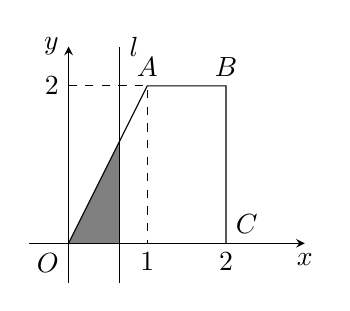
\begin{tikzpicture}[samples=200,>=stealth]
	\fill [gray] (0,0)--(0.65,0)--(0.65,1.3)--cycle;
	\draw [->] (-0.5,0)--(0,0) node [below left] {$O$} --(3,0) node [below] {$x$};
	\draw [->] (0,-0.5)--(0,2.5) node [left] {$y$};
	\draw (0,0)--(1,2) node [above] {$A$}--(2,2) node [above] {$B$}--(2,0) node [above right] {$C$};
	\draw (0.65,-0.5)--(0.65,2.5) node [right] {$l$};
	\draw [dashed] (0,2) node [left] {$2$} --(1,2)--(1,0) node [below] {$1$};
	\draw (2,0) node [below] {$2$};
	
	\end{tikzpicture}
\end{center}
则函数$S=f(t)$的图像大致为\blank{30}.
\fourch{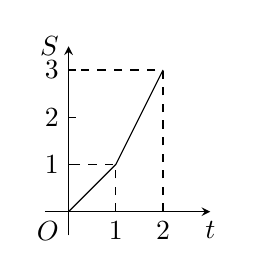
\begin{tikzpicture}[>=stealth]
	\draw [->] (-0.3,0)--(0,0) node [below left] {$O$} --(1.8,0) node [below] {$t$};
	\draw [->] (0,-0.3)--(0,2.1) node [left] {$S$};
	\draw (0.6,0) node [below] {$1$}--(0.6,0.1);
	\draw (1.2,0) node [below] {$2$}--(1.2,0.1);
	\draw (0,0.6) node [left] {$1$}--(0.1,0.6);
	\draw (0,1.2) node [left] {$2$}--(0.1,1.2);
	\draw (0,1.8) node [left] {$3$}--(0.1,1.8);
	\draw (0,0)--(0.6,0.6)--(1.2,1.8);
	\draw [dashed] (0.6,0)--(0.6,0.6)--(0,0.6);
	\draw [dashed] (1.2,0)--(1.2,1.8)--(0,1.8);
	\end{tikzpicture}}{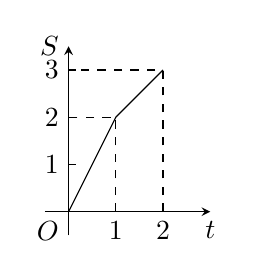
\begin{tikzpicture}[>=stealth]
	\draw [->] (-0.3,0)--(0,0) node [below left] {$O$} --(1.8,0) node [below] {$t$};
	\draw [->] (0,-0.3)--(0,2.1) node [left] {$S$};
	\draw (0.6,0) node [below] {$1$}--(0.6,0.1);
	\draw (1.2,0) node [below] {$2$}--(1.2,0.1);
	\draw (0,0.6) node [left] {$1$}--(0.1,0.6);
	\draw (0,1.2) node [left] {$2$}--(0.1,1.2);
	\draw (0,1.8) node [left] {$3$}--(0.1,1.8);
	\draw (0,0)--(0.6,1.2)--(1.2,1.8);
	\draw [dashed] (0.6,0)--(0.6,1.2)--(0,1.2);
	\draw [dashed] (1.2,0)--(1.2,1.8)--(0,1.8);
	\end{tikzpicture}}{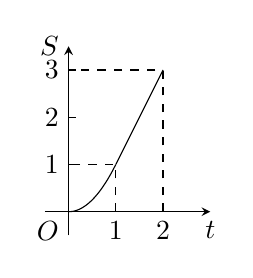
\begin{tikzpicture}[>=stealth,samples=200]
	\draw [->] (-0.3,0)--(0,0) node [below left] {$O$} --(1.8,0) node [below] {$t$};
	\draw [->] (0,-0.3)--(0,2.1) node [left] {$S$};
	\draw (0.6,0) node [below] {$1$}--(0.6,0.1);
	\draw (1.2,0) node [below] {$2$}--(1.2,0.1);
	\draw (0,0.6) node [left] {$1$}--(0.1,0.6);
	\draw (0,1.2) node [left] {$2$}--(0.1,1.2);
	\draw (0,1.8) node [left] {$3$}--(0.1,1.8);
	\draw [domain=0:1] plot ({\x*0.6},{\x*\x*0.6});
	\draw (0.6,0.6)--(1.2,1.8);
	\draw [dashed] (0.6,0)--(0.6,0.6)--(0,0.6);
	\draw [dashed] (1.2,0)--(1.2,1.8)--(0,1.8);
	\end{tikzpicture}}{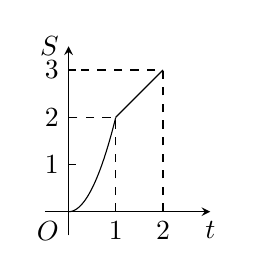
\begin{tikzpicture}[>=stealth,samples=200]
	\draw [->] (-0.3,0)--(0,0) node [below left] {$O$} --(1.8,0) node [below] {$t$};
	\draw [->] (0,-0.3)--(0,2.1) node [left] {$S$};
	\draw (0.6,0) node [below] {$1$}--(0.6,0.1);
	\draw (1.2,0) node [below] {$2$}--(1.2,0.1);
	\draw (0,0.6) node [left] {$1$}--(0.1,0.6);
	\draw (0,1.2) node [left] {$2$}--(0.1,1.2);
	\draw (0,1.8) node [left] {$3$}--(0.1,1.8);
	\draw [domain=0:1] plot ({\x*0.6},{2*\x*\x*0.6});
	\draw (0.6,1.2)--(1.2,1.8);
	\draw [dashed] (0.6,0)--(0.6,1.2)--(0,1.2);
	\draw [dashed] (1.2,0)--(1.2,1.8)--(0,1.8);
	\end{tikzpicture}}
\item {\tiny (003869)}函数$f(x)=a^x+b \ (a>1, \ b<-1)$, 则$y=f^{-1}(x)$的图像一定不经过第\blank{50}象限.
\item {\tiny (003884)}已知函数$y=f(x)$的定义域为$\{x|-3\le x\le 8, \ x\ne 5\}$, 值域为$\{y|-1\le y\le 2, \ y\ne 0\}$. 下列关于函数$y=f(x)$的说法: \textcircled{1} 当$x=-3$时, $y=-1$; \textcircled{2} 将$y=f(x)$的图像补上$(5,0)$, 得到的图像必定是一条连续的曲线; \textcircled{3} $y=f(x)$是$[-3,5)$上的单调函数; \textcircled{4} $y=f(x)$的图像与坐标轴只有一个交点. 其中正确的命题是\blank{50}.
\item {\tiny (003889)}已知函数$f(x)=\begin{cases}ax^2-2x-1, & x\ge 0,\\ x^2+bx+c, & x<0\end{cases}$是偶函数, 直线$y=t$与函数$y=f(x)$的图像自左向右依次交于四个不同点$A,B,C,D$. 若$AB=BC$, 则实数$t$的值为\blank{50}.
\item {\tiny (003894)}对于函数$f(x)=ax^2+(b+1)x+b-2 \ (a\ne 0)$, 若存在实数$x_0$, 使$f(x_0)=x_0$成立, 则称$x_0$为$f(x)$的不动点.\\
(1) 若对于任何实数$b$, 函数$f(x)$恒有两个相异的不动点, 求实数$a$的取值范围;\\
(2) 在(1)的条件下, 若函数$y=f(x)$的图像上$A,B$两点的横坐标是函数$f(x)$的不动点, 且直线$y=kx+\dfrac{1}{2a^2+1}$是线段$AB$的垂直平分线, 求实数$b$的取值范围.
\item {\tiny (003936)}函数$y=\ln(\cos x) \ \left(-\dfrac{\pi}{2}<x<\dfrac{\pi}{2}\right)$的大致图像是\blank{30}.
\fourch{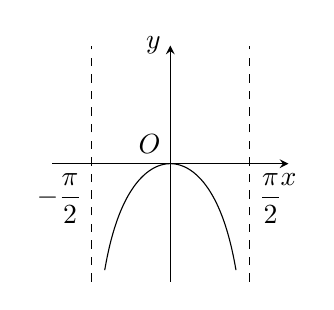
\begin{tikzpicture}[samples=200,>=stealth]
	\draw [->](-1.5,0)--(0,0) node [above left] {$O$}--(1.5,0) node [below] {$x$};
	\draw [->](0,-1.5)--(0,1.5) node [left] {$y$};
	\draw [dashed] (-1,-1.5)--(-1,1.5) (1,-1.5)--(1,1.5);
	\draw (-1,0) node [below left] {$-\dfrac{\pi}{2}$};
	\draw (1,0) node  [below right] {$\dfrac{\pi}{2}$};
	\draw [domain=-75:75] plot ({\x/90},{ln(cos(\x))});
	\end{tikzpicture}}{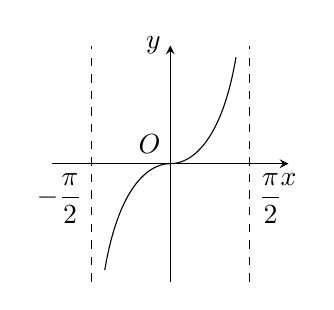
\begin{tikzpicture}[samples=200,>=stealth]
	\draw [->](-1.5,0)--(0,0) node [above left] {$O$}--(1.5,0) node [below] {$x$};
	\draw [->](0,-1.5)--(0,1.5) node [left] {$y$};
	\draw [dashed] (-1,-1.5)--(-1,1.5) (1,-1.5)--(1,1.5);
	\draw (-1,0) node [below left] {$-\dfrac{\pi}{2}$};
	\draw (1,0) node  [below right] {$\dfrac{\pi}{2}$};
	\draw [domain=-75:0] plot ({\x/90},{ln(cos(\x))});
	\draw [domain=0:75] plot ({\x/90},{-ln(cos(\x))});
	\end{tikzpicture}}{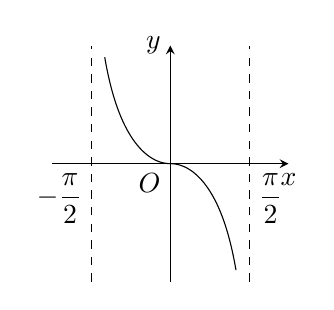
\begin{tikzpicture}[samples=200,>=stealth]
	\draw [->](-1.5,0)--(0,0) node [below left] {$O$}--(1.5,0) node [below] {$x$};
	\draw [->](0,-1.5)--(0,1.5) node [left] {$y$};
	\draw [dashed] (-1,-1.5)--(-1,1.5) (1,-1.5)--(1,1.5);
	\draw (-1,0) node [below left] {$-\dfrac{\pi}{2}$};
	\draw (1,0) node  [below right] {$\dfrac{\pi}{2}$};
	\draw [domain=-75:0] plot ({\x/90},{-ln(cos(\x))});
	\draw [domain=0:75] plot ({\x/90},{ln(cos(\x))});
	\end{tikzpicture}}{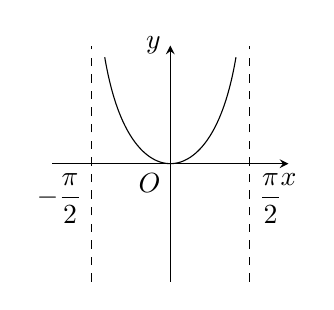
\begin{tikzpicture}[samples=200,>=stealth]
	\draw [->](-1.5,0)--(0,0) node [below left] {$O$}--(1.5,0) node [below] {$x$};
	\draw [->](0,-1.5)--(0,1.5) node [left] {$y$};
	\draw [dashed] (-1,-1.5)--(-1,1.5) (1,-1.5)--(1,1.5);
	\draw (-1,0) node [below left] {$-\dfrac{\pi}{2}$};
	\draw (1,0) node  [below right] {$\dfrac{\pi}{2}$};
	\draw [domain=-75:75] plot ({\x/90},{-ln(cos(\x))});
	\end{tikzpicture}}
\item {\tiny (004000)}请根据图中的函数图像, 将下列数值按从小到大的顺序排列:\blank{50}.
\begin{center}
    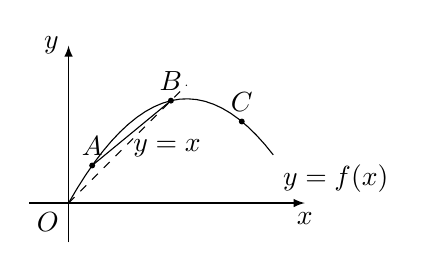
\begin{tikzpicture}[>=latex]
        \draw [->] (-0.5,0) -- (3,0) node [below] {$x$};
        \draw [->] (0,-0.5) -- (0,2) node [left] {$y$};
        \draw (0,0) node [below left] {$O$};
        \draw [domain = 0:2.6, name path = curve] plot (\x,{\x*(3-\x)/1.7}) node [below right] {$y=f(x)$};
        \draw [dashed] (0,0) -- (1.5,1.5);
        \filldraw (1.3,1.3) circle (0.03) node [above] {$B$} -- (0.3,{0.3*2.7/1.7}) circle (0.03) node [above] {$A$};
        \filldraw (2.2,{2.2*0.8/1.7}) circle (0.03) node [above] {$C$};
        \draw (0.7,0.7) node [right] {$y=x$};
    \end{tikzpicture}    
\end{center}
\textcircled{1} 曲线在点$A$处切线的斜率;\\
\textcircled{2} 曲线在点$B$处切线的斜率;\\
\textcircled{3} 曲线在点$C$处切线的斜率;\\
\textcircled{4} 割线$AB$的斜率;\\
\textcircled{5} 数值$0$;\\
\textcircled{6} 数值$1$.
\item {\tiny (004007)}已知$y=f'(x)$的图像如图所示, 求函数$y=f(x)$在$(-2,2)$上的单调区间和极值点.
\begin{center}
    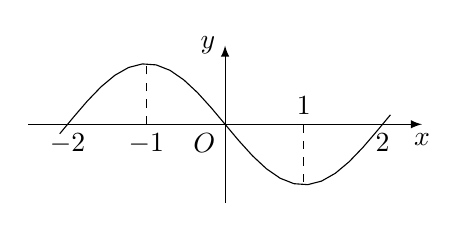
\begin{tikzpicture}[>=latex]
        \draw [->] (-2.5,0) -- (2.5,0) node [below] {$x$};
        \draw [->] (0,-1) -- (0,1) node [left] {$y$};
        \draw (0,0) node [below left] {$O$};
        \draw [domain = -2.1:2.1] plot (\x, {-sin(\x*90)/1.3});
        \draw [dashed] (-1,0) node [below] {$-1$} -- (-1,{1/1.3}) (1,0) node [above] {$1$}-- (1,{-1/1.3});
        \draw (-2,0) node [below] {$-2$} (2,0) node [below] {$2$};
    \end{tikzpicture}
\end{center}
\item {\tiny (004009)}设函数$y=x^3+ax^2+bx+c$的图像与$y=0$在原点相切, 若函数的极小值为$-4$, 求函数的表达式与单调减区间.
\item {\tiny (004067)}已知定义在$\mathbf{R}$上的函数$f(x)$满足: \textcircled{1} $f(x)+f(2-x)=0$; \textcircled{2} $f(x)-f(-2-x)=0$; \textcircled{3} 在$[-1,1]$上表达式为$f(x)=\begin{cases} \sqrt{1-x^2}, & x\in [-1,0], \\ 1-x, & x\in (0,1], \end{cases}$ 则函数$f(x)$与$g(x)=\begin{cases} {2^x}, & x\le 0 \\ \log_\frac 12x, & x>0 \end{cases}$的图像在区间$[-3,3]$上的交点的个数为\blank{50}.
\item {\tiny (004070)}已知$f(x)=2x^2+2x+b$是定义在$[-1,0]$上的函数, 若$f[f(x)]\le 0$在定义域上恒成立, 而且存在实数$x_0$满足: $f[f(x_0)]=x_0$且$f(x_0)\ne x_0$, 则实数$b$的取值范围是\blank{50}.
\item {\tiny (004089)}$[x]$是不超过$x$的最大整数, 则方程$(2^x)^2-\dfrac 74\cdot [2^x]-\dfrac 14=0$满足$x<1$的所有实数解是\blank{50}.
\item {\tiny (004097)}已知函数$f(x)=1-\dfrac 6{a^{x+1}+a}$($a>0$, $a\ne 1$)是定义在$\mathbf{R}$上的奇函数.\\
(1) 求实数$a$的值及函数$f(x)$的值域;\\
(2) 若不等式 $t\cdot f(x)\ge 3^x-3$在$x\in [1,2]$上恒成立, 求实数$t$的取值范围.
\item {\tiny (004151)}设不等式组$\begin{cases} x+y-6\ge 0, \\ x-y+2\ge 0, \\ x-3y+6\le 0 \end{cases}$表示的可行域为$\Omega$, 若指数函数$y=a^x$的图像与$\Omega$有公共点, 则$a$的取值范围是\blank{50}.
\item {\tiny (004184)}设$m$为给定的实常数, 若函数$y=f(x)$在其定义域内存在实数$x_0$, 使得$f(x_0+m)=f(x_0)+f(m)$成立, 则称函数$f(x)$为``$G(m)$函数''.\\
(1) 若函数$f(x)=2^x$为``$G(2)$函数'', 求实数$x_0$的值;\\
(2) 若函数$f(x)=\lg \dfrac a{x^2+1}$为``$G(1)$函数'', 求实数$a$的取值范围;\\
(3) 已知$f(x)=x+b$($b\in \mathbf{R}$)为``$G(0)$函数'', 设$g(x)=x|x-4|$. 若对任意的$x_1,x_2\in[0,t]$, 当$x_1\ne x_2$时, 都有$\dfrac{g(x_1)-g(x_2)}{f(x_1)-f(x_2)}>2$成立, 求实数$t$的最大值.
\item {\tiny (004214)}设定义域为$\mathbf{R}$的函数$f(x)$、$g(x)$都有反函数, 且函数$f(x-1)$和$g^{-1}(x-3)$图像关于直线$y=x$对称, 若$g(5)=2015$, 则$f(4)=$\blank{50}.
\item {\tiny (004220)}已知函数\textcircled{1} $f(x)=3\ln x$; \textcircled{2} $f(x)=3\mathrm{e}^{\cos x}$; \textcircled{3} $f(x)=3\mathrm{e}^x$; \textcircled{4} $f(x)=3\cos x$; 其中对于$f(x)$定义域内的任意一个自变量$x_1$都存在唯一一个自变量$x_2$, 使$\sqrt{f(x_1)f(x_2)}=3$成立的函数是\bracket{20}.
\fourch{\textcircled{3}}{\textcircled{2}\textcircled{3}}{\textcircled{1}\textcircled{2}\textcircled{4}}{\textcircled{4}}
\item {\tiny (004224)}对于两个定义域相同的函数$f(x)$、$g(x)$, 若存在实数$m$、$n$, 使$h(x)=mf(x)+ng(x)$, 则称函数$h(x)$是由``基函数$f(x)$、$g(x)$''生成的.\\
(1) $f(x)=x^2+3x$和$g(x)=3x+4$生成一个偶函数$h(x)$, 求$h(2)$的值;\\
(2) 若$h(x)=2x^2+3x-1$由$f(x)=x^2+ax$, $g(x)=x+b$($a,b\in \mathbf{R}$且$ab\ne 0$)生成, 求$a+2b$的取值范围.
\item {\tiny (004228)}函数$f(x)=\sqrt{1-\dfrac 2x}$的定义域是\blank{50}.
\item {\tiny (004270)}函数$f(x)=\sqrt{\dfrac{1-x}{3+x}}$的定义域为\blank{50}.
\item {\tiny (004272)}已知函数$g(x)$的图像与函数$f(x)=\log_2(3^x-1)$的图像关于直线$y=x$对称,则$g(3)=$\blank{50}.
\item {\tiny (004289)}已知函数$f(x)$的定义域为$D$, 若存在实常数$\lambda$及$a$($a\ne 0$), 对任意$x\in D$, 当$x+a\in D$且$x-a\in D$时, 都有$f(x+a)+f(x-a)=\lambda f(x)$成立, 则称函数$f(x)$具有性质$M(\lambda,a)$.\\
(1) 判断函数$f(x)=x^2$是否具有性质$M(\lambda,a)$, 并说明理由;\\
(2) 若函数$g(x)=\sin 2x+\sin x$具有性质$M(\lambda,a)$, 求$\lambda$及$a$应满足的条件;\\
(3) 已知定义域为$\mathbf{R}$的函数$y=h(x)$不存在零点, 且具有性质$M(t+\dfrac{1}{t},t)$(其中$t>0$, $t\ne 1$), 记$a_n=h(n)$($n\in \mathbf{N}^*$), 求证: 数列$\{a_n\}$为等比数列的充要条件是$\dfrac{a_2}{a_1}=t$或$\dfrac{a_2}{a_1}=\dfrac{1}{t}$.
\item {\tiny (004305)}定义$F(a,b)=\begin{cases} a, & a \le b, \\ b, & a>b,\end{cases}$, 已知函数$f(x)$、$g(x)$定义域都是$\mathbf{R}$, 给出下列命题:\\
(1) 若$f(x)$、$g(x)$都是奇函数, 则函数$F(f(x),g(x))$为奇函数;\\
(2) 若$f(x)$、$g(x)$都是减函数, 则函数$F(f(x),g(x))$为减函数;\\
(3) 若$f_{\min}(x)=m$, $g_{\min}(x)=n$, 则$F_{\min}(f(x),g(x))=F(m,n)$;\\
(4) 若$f(x)$、$g(x)$都是周期函数, 则函数$F(f(x),g(x))$是周期函数.\\
其中正确命题的个数为\bracket{20}.
\fourch{$1$个}{$2$个}{$3$个}{$4$个}
\item {\tiny (004313)}设$a\in \mathbf{R}$. 若$a$使得函数$f(x)=\sqrt{8-ax-2x^2}$是偶函数, 则函数$y=f(x)$的定义域是\blank{50}.
\item {\tiny (004332)}函数$y=\log_2(x-2)$的定义域为\blank{50}.
\item {\tiny (004335)}幂函数$y=x^k$的图像经过点$(4,\dfrac 12)$, 则它的单调减区间为\blank{50}.
\item {\tiny (004339)}已知偶函数$y=f(x)$的定义域为$\mathbf{R}$, 且当$x\ge 0$时, $f(x)=x-4$, 则不等式$xf(x)\le 5$的解为\blank{50}.
\item {\tiny (004347)}已知$y=f(x)$与$y=g(x)$皆是定义域、值域均为$\mathbf{R}$的函数. 若对任意$x\in \mathbf{R}$, $f(x)>g(x)$恒成立, 且$y=f(x)$与$y=g(x)$的反函数$y=f^{-1}(x)$、$y=g^{-1}(x)$均存在. 命题$P$: ``对任意$x\in \mathbf{R}$, $f^{-1}(x)<g^{-1}(x)$恒成立''; 命题$Q$: ``函数$y=f(x)+g(x)$的反函数一定存在''. 以下关于这两个命题的真假判断, 正确的是\bracket{20}.
\twoch{命题$P$真, 命题$Q$真}{命题$P$真, 命题$Q$假
}{命题$P$假, 命题$Q$真}{命题$P$假, 命题$Q$假}
\item {\tiny (004368)}已知函数$y=f(x)$的定义域为$(0,+\infty)$, 满足对任意$x\in (0,+\infty)$, 恒有$f[f(x)-\dfrac 1x]=4$. 若函数$y=f(x)-4$的零点个数为有限的$n$($n\in \mathbf{N}^*$)个, 则$n$的最大值为\bracket{20}.
\fourch{$1$}{$2$}{$3$}{$4$}
\item {\tiny (004377)}函数$f(x)=\sqrt{\dfrac{1-x}x}$的定义域为\blank{50}.
\item {\tiny (004380)}已知函数$f(x)$的定义域为$\mathbf{R}$, 满足对任意$x\in \mathbf{R}$, 恒有$f(x)+f(x+2)=4$. 若$f(1)+f(2)=1$, 则$f(2021)-f(2020)=$\blank{50}.
\item {\tiny (004385)}设函数$f(x)$的定义域为$\mathbf{R}$, $f(x)$满足对任意$x_1,x_2\in \mathbf{R}$, 当$x_1\ne x_2$时, 恒有$|f(x_1)-f(x_2)|>2|x_1-x_2|$. 对于命题: \textcircled{1} $f(x)$的解析式可以是$f(x)=x^3+2021x$; \textcircled{2} $f(x)$的解析式可以是$f(x)=2021^{-x}$, 下列判断正确的是\bracket{20}.
\twoch{\textcircled{1}、\textcircled{2}均为真命题}{\textcircled{1}、\textcircled{2}均为假命题}{\textcircled{1}为真命题、\textcircled{2}为假命题}{\textcircled{1}为假命题、\textcircled{2}为真命题}
\item {\tiny (004387)}设函数$f(x)$的定义域为$(0,+\infty)$, 若对任意$x\in (0,+\infty)$, 恒有$f(2x)=2f(x)$, 则称$f(x)$为``$2$阶缩放函数''.\\
(1) 已知函数$f(x)$为``$2$阶缩放函数'', 当$x\in (1,2]$时, $f(x)=1-\log_2 x$, 求$f(2\sqrt{2})$的值;\\
(2) 已知函数$f(x)$为``$2$阶缩放函数'', 当$x\in (1,2]$时, $f(x)=\sqrt{2x-x^2}$, 求证: 函数$y=f(x)-x$在$(1,+\infty)$上无零点.
\item {\tiny (004389)}函数$f(x)=x^{- \frac 12}$的定义域为\blank{50}.
\item {\tiny (004401)}下列函数中, 值域为$(0,+\infty)$的是\bracket{20}.
\fourch{$y=x^2$}{$y=\dfrac 2x$}{$y=2^x$}{$y=|\log_2x|$}
\item {\tiny (004403)}设集合$A=\{y|y=a^x,\ x>0\}$(其中常数$a>0,  \ a\ne 1$), $B=\{y|y=x^k,\ x\in A\}$(其中常数$k\in \mathbf{Q}$), 则``$k<0$''是``$A\cap B=\varnothing$''的\bracket{20}.
\twoch{充分非必要条件}{必要非充分条件}{充分必要条件}{既非充分又非必要条件}
\item {\tiny (004408)}记函数$f(x)$的定义域为$D$. 如果存在实数$a$、$b$使得$f(a-x)+f(a+x)=b$对任意满足$a-x\in D$且$a+x\in D$的$x$恒成立, 则称$f(x)$为$\Psi$函数.\\
(1) 设函数$f(x)=\dfrac 1x-1$, 试判断$f(x)$是否为$\Psi$函数, 若是求出$a,b$, 若不是请说明理由;\\
(2) 设函数$g(x)=\dfrac 1{2^x+t}$, 其中常数$t\ne 0$, 证明: $g(x)$是$\Psi$函数;\\
(3) 若$h(x)$是定义在$\mathbf{R}$上的$\Psi$函数, 且函数$h(x)$的图像关于直线$x=m$($m$为常数)对称, 试判断$h(x)$是否为周期函数? 并证明你的结论.
\item {\tiny (004411)}若函数$y=\log_2(x-m)+1$的反函数的图像经过点$(1,3)$, 则实数$m=$\blank{50}.
\item {\tiny (004412)}函数$f(x)=x+\dfrac 1{x-2}$的值域是\blank{50}.
\item {\tiny (004417)}函数$f(x)=\dfrac x{x+1}+\dfrac{x+1}{x+2}+\dfrac{x+2}{x+3}$图像的对称中心的坐标是\blank{50}.
\item {\tiny (004424)}设$\mu (x)$表示不小于$x$的最小整数, 例如$\mu(0.3)=1$, $\mu(-2.5)=2$.\\
(1) 解方程$\mu(x-1)=3$;\\
(2) 设$f(x)=\mu (x\cdot \mu (x))$, $n\in \mathbf{N}^*$, 试分别求出$f(x)$在区间$(0,1]$、$(1,2]$以及$(2,3]$上的值域; 若$f(x)$在区间$(0,n]$上的值域为$M_n$, 求集合$M_n$中的元素的个数;\\
(3) 设实数$a>0$, $g(x)=x+a\cdot \dfrac{\mu (x)}x-2$, $h(x)=\dfrac{\sin (\pi x)+2}{x^2-5x+7}$, 若对于任意$x_1,x_2\in (2,4]$都有$g(x_1)>h(x_2)$, 求实数$a$的取值范围.
\item {\tiny (004425)}函数$y=\log_2(4-x^2)$的定义域是\blank{50}.
\item {\tiny (004429)}已知函数$f(x)=a\cdot 2^x+3-a$($a\in \mathbf{R}$且$a\ne 0$)的反函数为$y=f^{-1}(x)$, 则函数$y=f^{-1}(x)$的图像经过的定点的坐标为\blank{50}.
\item {\tiny (004435)}集合$A=\{y|y=\log_{\frac 12}x-x,1\le x\le 2\}$, $B=\{x|x^2-5tx+1\le 0\}$, 若$A\cap B=A$, 则实数$t$的取值范围是\blank{50}.
\item {\tiny (004436)}若定义在实数集$\mathbf{R}$上的奇函数$y=f(x)$的图像关于直线$x=1$对称, 且当$0\le x\le 1$时, $f(x)=x^{\frac 13}$, 则方程$f(x)=\dfrac 13$在区间$(-4,10)$内的所有实根之和为\blank{50}.
\item {\tiny (004440)}已知函数$f(x)=\begin{cases}\log_{\frac 12}(1-x), & -1\le x\le n,  \\ 2^{2-|x-1|}-3, & n<x\le m,  \end{cases}$($n<m$)的值域是$[-1,1]$, 有下列结论:
\textcircled{1} 当$n=0$时, $m$的取值范围为$(0,2]$; \textcircled{2}  当$n=\dfrac 12$时, $m$的取值范围为$(\dfrac 12,2]$; \textcircled{3}  当$n\in [0,\dfrac 12)$时, $m$的取值范围为$[1,2]$; \textcircled{4}  当$n\in [0,\dfrac 12)$时, $m$的取值范围为$(n,2]$;
其中结论正确的所有的序号是\bracket{20}.
\fourch{\textcircled{1}\textcircled{2}}{\textcircled{3}\textcircled{4}}{\textcircled{2}\textcircled{3}}{\textcircled{2}\textcircled{4}}
\item {\tiny (004444)}定义区间$(m,n)$、$[m,n]$、$(m,n]$、$[m,n)$的长度均为$n-m$, 已知不等式$\dfrac 7{6-x}\ge 1$的解集为$A$.\\
(1) 求$A$的长度;\\
(2) 函数$f(x)=\dfrac{(a^2+a)x-1}{a^2x}$($a\in \mathbf{R}$, $a\ne 0$)的定义域与值域都是$[m,n]$($n>m$), 求区间$[m,n]$的最大长度;\\
(3) 关于$x$的不等式$\log_2x+\log_2(tx+3t)<2$的解集为$B$, 若$A\cap B$的长度为$6$, 求实数$t$的取值范围.
\item {\tiny (004445)}对于函数$y=f(x)$($x\in D$), 如果存在实数$a$、$b$($a\ne 0$, 且$a=1$, $b=0$不同时成立), 使得$f(x)=f(ax+b)$对$x\in D$恒成立, 则称函数$f(x)$为``$(a,b)$映像函数''.\\
(1) 判断函数$f(x)=x^2-2$是否是``$(a,b)$映像函数'', 如果是, 请求出相应的$a$、$b$的值, 若不是, 请说明理由;\\
(2) 已知函数$y=f(x)$是定义在$[0,+\infty)$上的``$(2,1)$映像函数'', 且当$x\in [0,1)$时, $f(x)=2^x$, 求函数$y=f(x)$($x\in [3,7)$)的反函数;\\
(3) 在(2)的条件下, 试构造一个数列$\{a_n\}$, 使得当$x\in [a_n,{a_{n+1}})$($n\in \mathbf{N}^*$)时, $2x+1$的取值范围为$[{a_{n+1}},{a_{n+2}})$, 并求$x\in [a_n,{a_{n+1}})$($n\in \mathbf{N}^*$)时, 函数$y=f(x)$的解析式, 及$y=f(x)$($x\in [0,+\infty)$)的值域.
\item {\tiny (004446)}函数$y=\sqrt{2+x}$的定义域为\blank{50}.
\item {\tiny (004452)}已知幂函数$y=f(x)$的图像经过点$P(4,2)$, 则它的反函数为$f^{-1}(x)=$\blank{50}.
\item {\tiny (004496)}已知函数$y=f(x)$存在反函数$y=f^{-1}(x)$, 若函数$y=f(x)+2^x$的图像经过点$(1,4)$, 则函数$y=f^{-1}(x)+\log_2x$的图像必过点\blank{50}.
\item {\tiny (004500)}对于定义域为$D$的函数$f(x)$, 若存在$x_1,x_2\in D$且$x_1\ne x_2$, 使得$f(x_1^2)=f(x_2^2)=2f(x_1+x_2)$, 则称函数$f(x)$具有性质$M$. 若函数$g(x)=|\log_2x-1|$, $x\in (0,a]$具有性质$M$, 则实数$a$的最小值为\blank{50}.
\item {\tiny (004509)}若存在常数$k$($k>0$), 使得对定义域$D$内的任意$x_1$、$x_2$($x_1\ne x_2$), 都有$|f(x_1)-f(x_2)|\le k|x_1-x_2|$成立, 则称函数$f(x)$在其定义域$D$是``$k-$利普希兹条件函数''.\\
(1) 若函数$f(x)=\sqrt x$($1\le x\le 4$)是``$k-$利普希兹条件函数'', 求常数$k$的取值范围;\\
(2) 判断函数$f(x)=\log_2x$是否是``$2-$利普希兹条件函数'', 若是, 请证明, 若不是, 请说明理由;\\
(3) 若$y=f(x)$($x\in \mathbf{R}$)是周期为2的``$1-$利普希兹条件函数'', 证明: 对任意的实数$x_1$、$x_2$, 都有$|f(x_1)-f(x_2)|\le 1$.
\item {\tiny (004516)}函数$f(x)=1+\log_2x$($x\ge 4$)的反函数的定义域为\blank{50}.
\item {\tiny (004523)}已知函数$f^{-1}(x)$为函数$f(x)$的反函数, 且函数$f(x-1)$的图像经过点$(1,1)$, 则函数$f^{-1}(x)$的图像一定经过点\bracket{20}
\fourch{$(0,1)$}{$(1,0)$}{$(1,2)$}{$(2,1)$}
\item {\tiny (004525)}已知函数$f(x)=\begin{cases} x^2, & x\text{为无理数}, \\ x, &x\text{为有理数},   \end{cases}$ 则以下$4$个命题:
\textcircled{1} $f(x)$是偶函数; \textcircled{2} $f(x)$在$[0,+\infty)$上是增函数; \textcircled{3} $f(x)$的值域为$\mathbf{R}$; \textcircled{4} 对于任意的正有理数$a$, $g(x)=f(x)-a$存在奇数个零点.
其中正确命题的个数为\bracket{20}.
\fourch{$0$}{$1$}{$2$}{$3$}
\item {\tiny (004530)}已知函数$f(x)$的定义域是$D$, 若对于任意的$x_1,x_2\in D$, 当$x_1<x_2$时, 都有$f(x_1)\le f(x_2)$, 则称函数$f(x)$在$D$上为``非减函数''.\\
(1) 判断$f_1(x)=x^2-4x, \ x\in [1,4]$与$f_2(x)=|x-1|+|x-2|, \ x\in [1,4]$是否是``非减函数''?\\
(2) 已知函数$g(x)=2^x+\dfrac a{2^{x-1}}$在$[2,4]$上为``非减函数'', 求实数$a$的取值范围;\\
(3) 已知函数$h(x)$在$[0,1]$上为``非减函数'', 且满足条件:
\textcircled{1}  $h(0)=0$; \textcircled{2}  $h(\dfrac x3)=\dfrac 12h(x)$; \textcircled{3}  $h(1-x)=1-h(x)$, 求 $h(\dfrac 1{2020})$的值.
\item {\tiny (004540)}已知$y=f(x)$是定义在$\mathbf{R}$上的奇函数, 且当$x\ge 0$时, $f(x)=-\dfrac 1{4^x}+\dfrac 1{2^x}$, 则此函数的值域为\blank{50}.
\item {\tiny (004563)}下列函数中, 值域为$[0,+\infty)$的是\bracket{20}.
\fourch{$y=2^x$}{$y=x^\frac 12$}{$y=\tan x$}{$y=\cos x$}
\item {\tiny (004661)}函数$f(x)={x^{-\frac 12}}$的定义域是\blank{50}.
\item {\tiny (004760)}已知以下三个陈述句:\\
$p$: 存在$a\in \mathbf{R}$且$a\ne 0$, 对任意的$x\in \mathbf{R}$, 均有$f(2^{x+a})<f(2^x)+f(a)$恒成立;\\
$q_1$: 函数$y=f(x)$是定义域为$\mathbf{R}$的减函数, 且对任意的$x\in \mathbf{R}$, 都有$f(x)>0$;\\
$q_2$: 函数$y=f(x)$是定义域为$\mathbf{R}$的增函数, 存在$x_0<0$, 使得$f(x_0)=0$;\\
用这三个陈述句组成两个命题, 命题$S$: ``若$q_1$, 则$p$''; 命题$T$: ``若$q_2$, 则$p$''. 关于$S,T$以下说法正确的是\bracket{20}.
\twoch{只有命题$S$是真命题}{只有命题$T$是真命题}{两个命题$S,T$都是真命题}{两个命题$S,T$都不是真命题}
\item {\tiny (005136)}在$\triangle ABC$中, 已知$BC=a$, $CA=b$, $AB=c$, $\angle ACB=\theta$. 现将$\triangle ABC$分别以$BC,CA,AB$所在直线为轴旋转一周, 设所得三个旋转体的体积依次为$V_1,V_2,V_3$.\\
(1) 设$T=\dfrac{V_3}{V_1+V_2}$, 试用$a,b,c$表示$T$;\\
(2) 若$\theta$为定值, 并令$\dfrac{a+b}c=x$, 将$T=\dfrac{V_3}{V_1+V_2}$表示为$x$的函数, 写出这个函数的定义域, 并求这个函数的最大值$M$;\\
(3) 若$\theta \in [\dfrac{\pi }3,\pi)$, 求(2)中$M$的最大值.
\item {\tiny (005272)}求函数$y=\dfrac{3x-1}{x+1}$的值域.
\item {\tiny (005273)}求函数$y=\dfrac{4x+3}{2x-1}$的值域.
\item {\tiny (005274)}求函数$y=\dfrac{x^2-1}{x^2+2}$的值域.
\item {\tiny (005275)}求函数$y=\dfrac{x^2-x+1}{2x^2-2x+3}$的值域.
\item {\tiny (005276)}求函数$y=\dfrac{x^2+4x+3}{x^2+x-6}$的值域.
\item {\tiny (005277)}若实数$x,y$满足$x^2+4y^2=4x$, 求$S=x^2+y^2$的值域.
\item {\tiny (005279)}求函数$y=3x^2-12x+18\sqrt {4x-x^2}-23$的值域.
\item {\tiny (005280)}求函数$y=|x-2|-|x+1|$的值域.
\item {\tiny (005282)}已知定义域为$\mathbf{R}$的函数$f(x)$满足:
\textcircled{1} $f(x+y)=f(x)\cdot f(y)$对任何实数$x,y$都成立;
\textcircled{2} 存在实数$x_1,x_2$, 使$f(x_1)\ne f(x_2)$.
求证:\\
(1) $f(0)=1$;\\
(2) $f(x)>0$.
\item {\tiny (005298)}函数$f(x)=\dfrac{\sqrt{x^2-5x+6}}{x-2}$的定义域是\bracket{20}.
\fourch{$\{x|2<x<3\}$}{$\{x|x<2x>3\}$}{$\{x|x\le 2x\ge 3\}$}{$\{x|x<2\text{或}x\ge 3\}$}
\item {\tiny (005299)}若函数$f(x)$的定义域是$[-1,1]$, 则函数$f(x+1)$的定义域是\bracket{20}.
\fourch{$[-1,1]$}{$[0,2]$}{$[-2,0]$}{$[0,1]$}
\item {\tiny (005301)}函数$y=-x^2-2x+3(-5\le x\le 0)$的值域是\bracket{20}.
\fourch{$(-\infty ,4]$}{$[3,12]$}{$[-12,4]$}{$[4,12]$}
\item {\tiny (005303)}函数$y=x+\dfrac{|x|}x$的图像是\bracket{20}.
\fourch{\begin{tikzpicture}[scale = 0.7,>=latex]
\draw [->] (-2,0) -- (2,0) node [below] {$x$};
\draw [->] (0,-2) -- (0,2) node [left] {$y$};
\draw (0,0) node [below right] {$O$};
\draw (-1,0) node [below] {$-1$} (0,1) node [right] {$1$};
\draw (-2,-1) -- (1,2);
\filldraw [white] (0,1) circle (0.05);
\draw (0,1) circle (0.05);
\end{tikzpicture}}{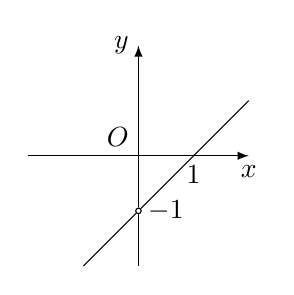
\begin{tikzpicture}[scale = 0.7,>=latex]
\draw [->] (-2,0) -- (2,0) node [below] {$x$};
\draw [->] (0,-2) -- (0,2) node [left] {$y$};
\draw (0,0) node [above left] {$O$};
\draw (1,0) node [below] {$1$} (0,-1) node [right] {$-1$};
\draw (-1,-2) -- (2,1);
\filldraw [white] (0,-1) circle (0.05);
\draw (0,-1) circle (0.05);
\end{tikzpicture}}{\begin{tikzpicture}[scale = 0.7,>=latex]
\draw [->] (-2,0) -- (2,0) node [below] {$x$};
\draw [->] (0,-2) -- (0,2) node [left] {$y$};
\draw (0,0) node [below right] {$O$};
\draw (1,0.1) -- (1,0) node [below] {$1$} (0,-1) node [right] {$-1$} (0,1) node [right] {$1$} (-1,0.1) -- (-1,0) node [below] {$-1$};
\draw (-1,-2) -- (0,-1) (0,1) -- (1,2);
\filldraw [white] (0,-1) circle (0.05);
\draw (0,-1) circle (0.05);
\filldraw [white] (0,1) circle (0.05);
\draw (0,1) circle (0.05);
\end{tikzpicture}}{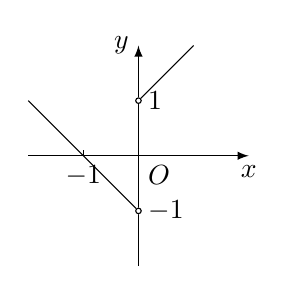
\begin{tikzpicture}[scale = 0.7,>=latex]
\draw [->] (-2,0) -- (2,0) node [below] {$x$};
\draw [->] (0,-2) -- (0,2) node [left] {$y$};
\draw (0,0) node [below right] {$O$};
\draw (0,-1) node [right] {$-1$} (0,1) node [right] {$1$} (-1,0.1) -- (-1,0) node [below] {$-1$};
\draw (-2,1) -- (0,-1) (0,1) -- (1,2);
\filldraw [white] (0,-1) circle (0.05);
\draw (0,-1) circle (0.05);
\filldraw [white] (0,1) circle (0.05);
\draw (0,1) circle (0.05);
\end{tikzpicture}}
\item {\tiny (005304)}函数$y=\sqrt {1-x^2}+\sqrt {x+1}$的定义域为\blank{50}.
\item {\tiny (005305)}函数$y=\dfrac 1{\sqrt {2x^2+3}}$的定义域为\blank{50}.
\item {\tiny (005306)}函数$y=\dfrac{x+5}{3x^2-2x-1}$的定义域为\blank{50}.
\item {\tiny (005307)}函数$y=\sqrt {6x-x^2-9}$的定义域为\blank{50}.
\item {\tiny (005308)}函数$y=\sqrt {4-x^2}+\dfrac 1{|x|-1}$的定义域为\blank{50}.
\item {\tiny (005309)}函数$y=\dfrac{x^3-1}{x+|x|}$的定义域为\blank{50}.
\item {\tiny (005310)}函数$y=\dfrac 1{|x|-x^2}$的定义域为\blank{50}.
\item {\tiny (005311)}函数$y=\sqrt {1-(\dfrac{x-1}{x+1})^2}$的定义域为\blank{50}.
\item {\tiny (005312)}函数$y=\dfrac{\sqrt {x^2-2x-15}}{|x+3|-8}$的定义域为\blank{50}.
\item {\tiny (005313)}函数$y=1-\dfrac 1{x+2}$的值域为\blank{50}.
\item {\tiny (005314)}函数$y=\dfrac 3{2x}$的值域为\blank{50}.
\item {\tiny (005315)}函数$y=\dfrac{x+3}{x-3}$的值域为\blank{50}.
\item {\tiny (005316)}函数$y=\dfrac{5x+3}{x-3}$的值域为\blank{50}.
\item {\tiny (005317)}函数$y=4+\sqrt {2x+1}$的值域为\blank{50}.
\item {\tiny (005318)}函数$y=\sqrt {x-\dfrac 12x^2}$的值域为\blank{50}.
\item {\tiny (005319)}函数$y=\sqrt {-x^2+x+2}$的值域为\blank{50}.
\item {\tiny (005320)}函数$y=\dfrac{2x^2+2x+3}{x^2+x+1}$的值域为\blank{50}.
\item {\tiny (005329)}若$-b<a<0$, 且函数$d(x)$的定义域是$[a,b]$, 则函数$F(x)=f(x)+f(-x)$的定义域是\bracket{20}.
\fourch{$[a,b]$}{$[-b,-a]$}{$[-b,b]$}{$[a,-a]$}
\item {\tiny (005330)}若$f(x)$的定义域是$[ 0,1 ]$, 且$f(x+m)+f(x-m)$的定义域是$\varnothing$, 则正数$m$的取值范围是\bracket{20}.
\fourch{$0<m<1$}{$0<m\le \dfrac 12$}{$0<m<\dfrac 12$}{$m>\dfrac 12$}
\item {\tiny (005331)}函数$y=\dfrac{x^2-1}{x^2+1}$的值域是\bracket{20}.
\fourch{$(-1,1)$}{$[-1,1]$}{$[-1,1)$}{$(-1,1]$}
\item {\tiny (005333)}函数$f(x)=|1-x|-|x-3|(x\in \mathbf{R})$的值域是\bracket{20}.
\fourch{$[-2,2]$}{$[-1,3]$}{$[-3,1]$}{$[0,4]$}
\item {\tiny (005334)}若函数$f(x)$的定义域是$[0,1]$, 分别求函数$f(1-2x)$和$f(x+a)$($a>0$)的定义域.
\item {\tiny (005335)}若函数$f(x+1)$的定义域是$[-2,3)$, 求函数$f(\dfrac 1x+2)$的定义域.
\item {\tiny (005336)}求函数$y=\dfrac{2x}{x^2+x+1}$的值域.
\item {\tiny (005337)}求函数$y=\dfrac{x^2+x-1}{x^2+x+1}$的值域.
\item {\tiny (005338)}求函数$y=\dfrac{x^2-1}{x^2-5x+4}$的值域.
\item {\tiny (005341)}求函数$y=3x-2+\sqrt {3-2x}$的值域.
\item {\tiny (005342)}求函数$y=2x+\sqrt {2x-1}$的值域.
\item {\tiny (005343)}求函数$y=(x-1)(x-2)(x-3)(x-4)+15$的值域.
\item {\tiny (005349)}已知函数$f(x)$的定义域是一切非零实数, 且满足$3f(x)+2f(\dfrac 1x)=4x$, 求, $f(x)$的表达式.
\item {\tiny (005350)}作出函数$y=1+\dfrac{|x|}x$的图像.
\item {\tiny (005351)}作出函数$y=x-|1-x|$的图像.
\item {\tiny (005352)}作出函数$y=|x^2-4x+3|$的图像.
\item {\tiny (005353)}作出函数$y=\dfrac{x^3+x}{|x|}$的图像.
\item {\tiny (005354)}作出函数$y=\dfrac{(x+\dfrac 12)}{|x|-x}^0$的图像.
\item {\tiny (005355)}已知$f(x)=-x^2+2x+3$, 画出函数$y=\dfrac 12[f(x)+|f(x)|]$的图像.
\item {\tiny (005356)}已知$f(x)=|x|$, $x\in [-1,1]$, 作出函数$y=f(x+1)+1$的图像.
\item {\tiny (005363)}画出函数$y=x^2-2|x|-1$的图像.
\item {\tiny (005364)}求函数$y=\dfrac{x-2}{2x+1}$的值域.
\item {\tiny (005365)}已知函数$f(x)=(x-1)^2$($x\le 1$), 又$f(x)$和$\varphi (x)$的图像关于直线$y=x$对称, 求$\varphi (x)$的表达式.
\item {\tiny (005445)}已知幂函数$f(x)$的图像经过点$(2,\dfrac{\sqrt 2}2)$, 则$f(4)$的值等于\bracket{20}.
\fourch{$16$}{$\dfrac 1{16}$}{$\dfrac 12$}{$2$}
\item {\tiny (005446)}下列幂函数中, 定义域为$\{x|x>0\}$的是\bracket{20}.
\fourch{$y=x^{\frac 23}$}{$y=x^{\frac 32}$}{$y=x^{-\frac 23}$}{$y=x^{-\frac 32}$}
\item {\tiny (005447)}幂函数$y=x^n(n\in \mathbf{Z})$的图像一定不经过\bracket{20}.
\fourch{第一象限}{第二象限}{第三象限}{第四象限}
\item {\tiny (005448)}函数$f(x)=x^{\frac 23}$的图像是\bracket{20}.
\fourch{\begin{tikzpicture}[scale = 0.7, >=latex]
\draw [->] (-2,0) -- (2,0) node [below] {$x$};
\draw [->] (0,-2) -- (0,2) node [left] {$y$};
\draw (0,0) node [below left] {$O$};
\draw (1,0.2) -- (1,0) node [below] {$1$};
\draw (0.2,1) -- (0,1) node [left] {$1$};
\draw [domain = 0:4,samples = 400] plot ({\x^(1/2)},{\x^(1/3)});
\end{tikzpicture}}{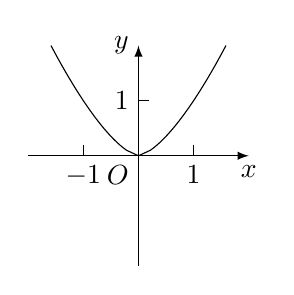
\begin{tikzpicture}[scale = 0.7, >=latex]
\draw [->] (-2,0) -- (2,0) node [below] {$x$};
\draw [->] (0,-2) -- (0,2) node [left] {$y$};
\draw (0,0) node [below left] {$O$};
\draw (1,0.2) -- (1,0) node [below] {$1$};
\draw (0.2,1) -- (0,1) node [left] {$1$};
\draw (-1,0.2) -- (-1,0) node [below] {$-1$};
\draw [domain = 0:4,samples = 400] plot ({\x^(1/3)},{\x^(1/2)});
\draw [domain = 0:4,samples = 400] plot ({-\x^(1/3)},{\x^(1/2)});
\end{tikzpicture}}{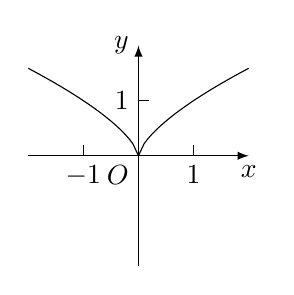
\begin{tikzpicture}[scale = 0.7, >=latex]
\draw [->] (-2,0) -- (2,0) node [below] {$x$};
\draw [->] (0,-2) -- (0,2) node [left] {$y$};
\draw (0,0) node [below left] {$O$};
\draw (1,0.2) -- (1,0) node [below] {$1$};
\draw (0.2,1) -- (0,1) node [left] {$1$};
\draw (-1,0.2) -- (-1,0) node [below] {$-1$};
\draw [domain = 0:4,samples = 400] plot ({\x^(1/2)},{\x^(1/3)});
\draw [domain = 0:4,samples = 400] plot ({-\x^(1/2)},{\x^(1/3)});
\end{tikzpicture}}{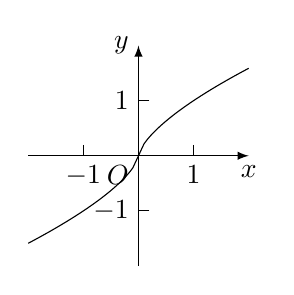
\begin{tikzpicture}[scale = 0.7, >=latex]
\draw [->] (-2,0) -- (2,0) node [below] {$x$};
\draw [->] (0,-2) -- (0,2) node [left] {$y$};
\draw (0,0) node [below left] {$O$};
\draw (1,0.2) -- (1,0) node [below] {$1$};
\draw (0.2,1) -- (0,1) node [left] {$1$};
\draw (-1,0.2) -- (-1,0) node [below] {$-1$};
\draw (0.2,-1) -- (0,-1) node [left] {$-1$};
\draw [domain = 0:4,samples = 400] plot ({\x^(1/2)},{\x^(1/3)});
\draw [domain = 0:4,samples = 400] plot ({-\x^(1/2)},{-\x^(1/3)});
\end{tikzpicture}}
\item {\tiny (005449)}幂函数$y=x^m$和$y=x^n$在第一象限内的图像$C_1$和$C_2$图像所示, 则$m,n$之间的关系是\bracket{20}.
\begin{center}
    \begin{tikzpicture}[>=latex]
        \draw [->] (-1,0) -- (3,0) node [below] {$x$};
        \draw [->] (0,-1) -- (0,3) node [left] {$y$};
        \draw (0,0) node [below left] {$O$};
        \draw (1,0.2) -- (1,0) node [below] {$1$};
        \draw (0.2,1) -- (0,1) node [left] {$1$};
        \draw [domain = 0.5:2, samples = 400] plot (\x,{\x^(-5/4)});
        \draw [domain = 0.5:2, samples = 400] plot ({\x^(-5/4)},\x);
        \draw (0.5,{0.5^(-5/4)}) node [right] {$C_2$} ({0.5^(-5/4)},0.5) node [above] {$C_1$};
    \end{tikzpicture}
\end{center}
\fourch{$n<m<0$}{$m<n<0$}{$n>m>0$}{$m>n>0$}
\item {\tiny (005450)}图中, $C_1,C_2,C_3$为幂函数$y=x^a$在第一象限的图像, 则解析式中的指数$\alpha$依次可以取\bracket{20}.
\begin{center}
    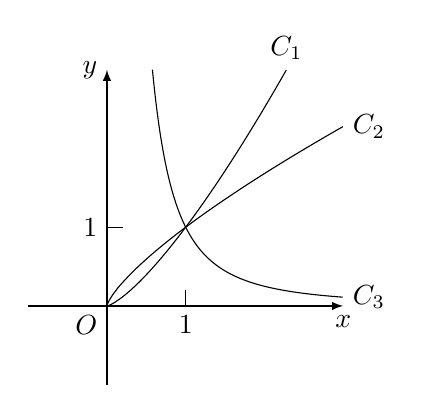
\begin{tikzpicture}[>=latex]
        \draw [->] (-1,0) -- (3,0) node [below] {$x$};
        \draw [->] (0,-1) -- (0,3) node [left] {$y$};
        \draw (0,0) node [below left] {$O$};
        \draw (1,0.2) -- (1,0) node [below] {$1$};
        \draw (0.2,1) -- (0,1) node [left] {$1$};
        \draw [domain = {sqrt(3)/3}:3, samples = 400] plot (\x,{\x^(-2)});
        \draw [domain = 0:3, samples = 400] plot (\x,{\x^(3/4)});
        \draw [domain = 0:{3^(3/4)}, samples = 400] plot (\x,{\x^(4/3)});
        \draw (3,{1/9}) node [right] {$C_3$} (3,{3^(3/4)}) node [right] {$C_2$} ({3^(3/4)},3) node [above] {$C_1$};
    \end{tikzpicture}
\end{center}
\fourch{$\dfrac 43,-2,\dfrac 34$}{$-2,\dfrac 34,\dfrac 43$}{$-2,\dfrac 43,\dfrac 34$}{$\dfrac 34,\dfrac 43,-2$}
\item {\tiny (005451)}函数$y=x^{\frac 56}$的定义域为\blank{50}, 值域为\blank{50}.
\item {\tiny (005452)}函数$y=x^{\frac 35}$的定义域为\blank{50}, 值域为\blank{50}.
\item {\tiny (005453)}函数$y=x^{\frac 85}$的定义域为\blank{50}, 值域为\blank{50}.
\item {\tiny (005454)}函数$y=x^{-\frac 54}$的定义域为\blank{50}, 值域为\blank{50}.
\item {\tiny (005455)}函数$y=x^{-\frac 53}$的定义域为\blank{50}, 值域为\blank{50}.
\item {\tiny (005456)}函数$y=x^{-\frac 23}$的定义域为\blank{50}, 值域为\blank{50}.
\item {\tiny (005457)}函数$y=-2(x+5)^{-\frac 14}$的定义域为\blank{50}, 值域为\blank{50}.
\item {\tiny (005458)}函数$y=5(2x-1)^{\frac 34}$的定义域为\blank{50}, 值域为\blank{50}.
\item {\tiny (005459)}将下列函数图像的标号, 填在相应函数后面的横线上:\\
(1) $y=x^{\frac 23}$:\blank{50}; (2) $y=x^{-2}$:\blank{50}; (3) $y=x^{\frac 12}$:\blank{50};\\
(4) $y=x^{-1}$:\blank{50}; (5) $y=x^{\frac 13}$:\blank{50}; (6)$y=x^{\frac 32}$:\blank{50};\\ (7)$y=x^{\frac 43}$:\blank{50}; (8)$y=x^{-\frac 12}$:\blank{50}; (9)$y=x^{\frac 53}$:\blank{50}.
\begin{center}
    \begin{tikzpicture}[>=latex,scale = 0.6]
        \draw [->] (-2.5,0) -- (2.5,0) node [below] {$x$};
        \draw [->] (0,-2.5) -- (0,2.5) node [left] {$y$};
        \draw (0,0) node [below left] {$O$};
        \draw (0.2,1) -- (0,1) node [left] {$1$} (0.2,-1) -- (0,-1) node [left] {$-1$};
        \draw (1,0.2) -- (1,0) node [below] {$1$} (-1,0.2) -- (-1,0) node [below] {$1$};
        \draw (0,-2.5) node [below] {(A)};
        \draw [domain = 0:2.4, samples = 400] plot (\x,{\x^(1/2)});
    \end{tikzpicture}
    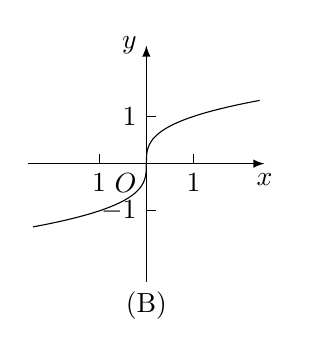
\begin{tikzpicture}[>=latex,scale = 0.6]
        \draw [->] (-2.5,0) -- (2.5,0) node [below] {$x$};
        \draw [->] (0,-2.5) -- (0,2.5) node [left] {$y$};
        \draw (0,0) node [below left] {$O$};
        \draw (0,-2.5) node [below] {(B)};
        \draw (0.2,1) -- (0,1) node [left] {$1$} (0.2,-1) -- (0,-1) node [left] {$-1$};
        \draw (1,0.2) -- (1,0) node [below] {$1$} (-1,0.2) -- (-1,0) node [below] {$1$};
        \draw [domain = 0:2.4, samples = 400] plot (\x,{\x^(1/3)});
        \draw [domain = 0:2.4, samples = 400] plot (-\x,{-\x^(1/3)});
    \end{tikzpicture}
    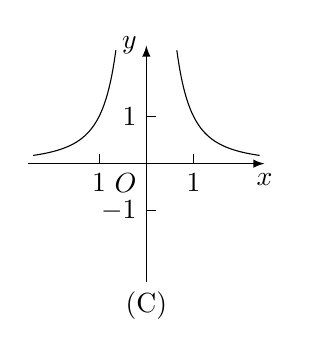
\begin{tikzpicture}[>=latex,scale = 0.6]
        \draw [->] (-2.5,0) -- (2.5,0) node [below] {$x$};
        \draw [->] (0,-2.5) -- (0,2.5) node [left] {$y$};
        \draw (0,0) node [below left] {$O$};
        \draw (0,-2.5) node [below] {(C)};
        \draw (0.2,1) -- (0,1) node [left] {$1$} (0.2,-1) -- (0,-1) node [left] {$-1$};
        \draw (1,0.2) -- (1,0) node [below] {$1$} (-1,0.2) -- (-1,0) node [below] {$1$};
        \draw [domain = {1/sqrt(2.4)}:2.4, samples = 400] plot (\x,{\x^(-2)});
        \draw [domain = {1/sqrt(2.4)}:2.4, samples = 400] plot (-\x,{\x^(-2)});
    \end{tikzpicture}\\
    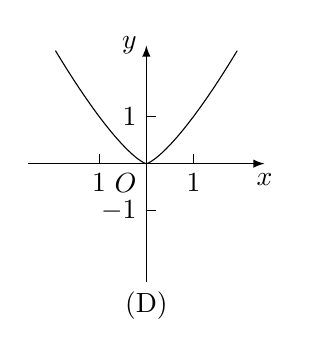
\begin{tikzpicture}[>=latex,scale = 0.6]
        \draw [->] (-2.5,0) -- (2.5,0) node [below] {$x$};
        \draw [->] (0,-2.5) -- (0,2.5) node [left] {$y$};
        \draw (0,0) node [below left] {$O$};
        \draw (0,-2.5) node [below] {(D)};
        \draw (0.2,1) -- (0,1) node [left] {$1$} (0.2,-1) -- (0,-1) node [left] {$-1$};
        \draw (1,0.2) -- (1,0) node [below] {$1$} (-1,0.2) -- (-1,0) node [below] {$1$};
        \draw [domain = 0:{2.4^(3/4)}, samples = 400] plot (\x,{\x^(4/3)});
        \draw [domain = 0:{2.4^(3/4)}, samples = 400] plot (-\x,{\x^(4/3)});
    \end{tikzpicture}
    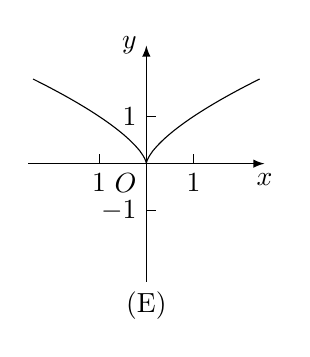
\begin{tikzpicture}[>=latex,scale = 0.6]
        \draw [->] (-2.5,0) -- (2.5,0) node [below] {$x$};
        \draw [->] (0,-2.5) -- (0,2.5) node [left] {$y$};
        \draw (0,0) node [below left] {$O$};
        \draw (0,-2.5) node [below] {(E)};
        \draw (0.2,1) -- (0,1) node [left] {$1$} (0.2,-1) -- (0,-1) node [left] {$-1$};
        \draw (1,0.2) -- (1,0) node [below] {$1$} (-1,0.2) -- (-1,0) node [below] {$1$};
        \draw [domain = 0:2.4, samples = 400] plot (\x,{\x^(2/3)});
        \draw [domain = 0:2.4, samples = 400] plot (-\x,{\x^(2/3)});
    \end{tikzpicture}
    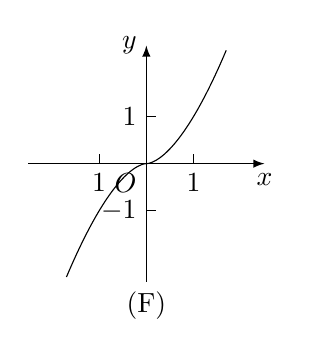
\begin{tikzpicture}[>=latex,scale = 0.6]
        \draw [->] (-2.5,0) -- (2.5,0) node [below] {$x$};
        \draw [->] (0,-2.5) -- (0,2.5) node [left] {$y$};
        \draw (0,0) node [below left] {$O$};
        \draw (0,-2.5) node [below] {(F)};
        \draw (0.2,1) -- (0,1) node [left] {$1$} (0.2,-1) -- (0,-1) node [left] {$-1$};
        \draw (1,0.2) -- (1,0) node [below] {$1$} (-1,0.2) -- (-1,0) node [below] {$1$};
        \draw [domain = 0:{2.4^(3/5)}, samples = 400] plot (\x,{\x^(5/3)});
        \draw [domain = 0:{2.4^(3/5)}, samples = 400] plot (-\x,{-\x^(5/3)});
    \end{tikzpicture}\\
    \begin{tikzpicture}[>=latex,scale = 0.6]
        \draw [->] (-2.5,0) -- (2.5,0) node [below] {$x$};
        \draw [->] (0,-2.5) -- (0,2.5) node [left] {$y$};
        \draw (0,0) node [below left] {$O$};
        \draw (0,-2.5) node [below] {(G)};
        \draw (0.2,1) -- (0,1) node [left] {$1$} (0.2,-1) -- (0,-1) node [left] {$-1$};
        \draw (1,0.2) -- (1,0) node [below] {$1$} (-1,0.2) -- (-1,0) node [below] {$1$};
        \draw [domain = {1/2.4}:2.4] plot (\x,{1/\x});
        \draw [domain = {1/2.4}:2.4] plot (-\x,{-1/\x});
    \end{tikzpicture}
    \begin{tikzpicture}[>=latex,scale = 0.6]
        \draw [->] (-2.5,0) -- (2.5,0) node [below] {$x$};
        \draw [->] (0,-2.5) -- (0,2.5) node [left] {$y$};
        \draw (0,0) node [below left] {$O$};
        \draw (0,-2.5) node [below] {(H)};
        \draw (0.2,1) -- (0,1) node [left] {$1$} (0.2,-1) -- (0,-1) node [left] {$-1$};
        \draw (1,0.2) -- (1,0) node [below] {$1$} (-1,0.2) -- (-1,0) node [below] {$1$};
        \draw [domain = {1/2.4^2}:2.4] plot (\x,{1/\x^(1/2)});
    \end{tikzpicture}
    \begin{tikzpicture}[>=latex,scale = 0.6]
        \draw [->] (-2.5,0) -- (2.5,0) node [below] {$x$};
        \draw [->] (0,-2.5) -- (0,2.5) node [left] {$y$};
        \draw (0,0) node [below left] {$O$};
        \draw (0,-2.5) node [below] {(I)};
        \draw (0.2,1) -- (0,1) node [left] {$1$} (0.2,-1) -- (0,-1) node [left] {$-1$};
        \draw (1,0.2) -- (1,0) node [below] {$1$} (-1,0.2) -- (-1,0) node [below] {$1$};
        \draw [domain = 0:{2.4^(2/3)}] plot (\x,{\x^(3/2)});
    \end{tikzpicture}
\end{center}
\item {\tiny (005460)}若幂函数$y=x^n$的图像在$0<x<1$时位于直线$y=x$的下方, 则$n$的取值范围是\blank{50}.
\item {\tiny (005461)}若幂函数$y=x^n$的图像在$0<x<1$时位于直线$y=x$的上方, 则$n$的取值范围是\blank{50}.
\item {\tiny (005462)}函数$f(x)=x^{k^2-2k-3}$($k\in \mathbf{Z}$)的图像如图所示, 则$k=$\blank{50}.
\begin{center}
    \begin{tikzpicture}[>=latex]
        \draw [->] (-2.5,0) -- (2.5,0) node [below] {$x$};
        \draw [->] (0,-0.5) -- (0,2.5) node [left] {$y$};
        \draw (0,0) node [below left] {$O$};
        \draw (0,-0.5) node [below] {(C)};
        \draw (0.2,1) -- (0,1) node [left] {$1$};
        \draw (1,0.2) -- (1,0) node [below] {$1$} (-1,0.2) -- (-1,0) node [below] {$1$};
        \draw [domain = {1/2.4^(1/4)}:2.4, samples = 400] plot (\x,{\x^(-4)});
        \draw [domain = {1/2.4^(1/4)}:2.4, samples = 400] plot (-\x,{\x^(-4)});
    \end{tikzpicture}
\end{center}
\item {\tiny (005471)}已知函数$y=x^{n^2-2n-3}$($n\in \mathbf{Z}$)的图像与两坐标轴都无公共点, 且其图像关于$y$轴对称, 求$n$的值, 并画出相应的函数图像.
\item {\tiny (005477)}若函数$f(x)$在定义域$\mathbf{R}$上为增函数, 且$f(x)<0$, 则下列函数在$\mathbf{R}$上为增函数的是\bracket{20}.
\fourch{$y=|f(x)|$}{$y=\dfrac 1{f(x)}$}{$y=[ f(x) ]^2$}{$y=[ f(x) ]^3$}
\item {\tiny (005484)}已知$f(x)=-x^3-x+1$($x\in \mathbf{R}$), 求证$y=f(x)$在定义域上为减函数.
\item {\tiny (005486)}求证: $f(x)=\sqrt x-\dfrac 1x$在定义域上是增函数.
\item {\tiny (005493)}下列函数中既是奇函数, 又在定义域上为增函数的是\bracket{20}.
\fourch{$f(x)=3x+1$}{$f(x)=\dfrac 1x$}{$f(x)=1-\dfrac 1x$}{$f(x)=x^3$}
\item {\tiny (005496)}已知$f(x)$是奇函数, 则下列各点中在函数$y=f(x)$的图像上的点的是\bracket{20}.
\fourch{$(a,f(-a))$}{$(-a,-f(a))$}{$(\dfrac 1a,-f(\dfrac 1a))$}{$(-\sin a,-f(-\sin a))$}
\item {\tiny (005498)}若奇函数$f(x)$的定义域是$\mathbf{R}$, 则$f(0)=$\blank{50}.
\item {\tiny (005505)}若函数$y=f(x)$是偶函数, 其图像与$x$轴有四个交点, 则方程$f(x)=0$的所有实数根之和为\bracket{20}.
\fourch{$4$}{$2$}{$1$}{$0$}
\item {\tiny (005508)}$f(x)+f(2-x)+2=0$对任何实数$x$都成立, 则$f(x)$的图像\bracket{20}.
\twoch{关于直线$x=1$成轴对称图形}{关于直线$x=2$成轴对称图形}{关于点$(1, -1)$成中心对称图形}{关于点$(-1,1)$成中心对称图形}
\item {\tiny (005519)}已知奇函数$f(x)$在定义域$(-l, l)$上是减函数, 求满足$f(1-m)+f(1-m^2)<0$的实数$m$的取值范围.
\item {\tiny (005522)}求证: 定义域为$(-l,l)$的任何函数都能表示成一个奇函数与一个偶函数之和.
\item {\tiny (005524)}函数$y=\sqrt {x^2-2x+3}$($x\le 1$)的反函数的定义域是\bracket{20}.
\fourch{$[0,+\infty)$}{$(2,+\infty)$}{$(-\infty ,1]$}{$[\sqrt 2,+\infty)$}
\item {\tiny (005527)}若函数$y=g(x)$的图像与函数$f(x)=(x-1)^2$($x\le 1$)的图像关于直线$y=x$对称.则$g(x)$的表达式是\bracket{20}.
\twoch{$g(x)=1-\sqrt x$($x\ge 0$)}{$g(x)=1+\sqrt x$($x\ge 0$)}{$g(x)=\sqrt {1-x}$($x\le 1$)}{$g(x)=\sqrt {1+x}$($x\ge -1$)}
\item {\tiny (005530)}若函数$f(x)$的图像经过点$(0, -1)$, 则函数$f(x+4)$的反函数的图像必经过点\bracket{20}.
\fourch{$(—1,4)$}{$(-4,-1)$}{$(-1,-4)$}{$(1,-4)$}
\item {\tiny (005531)}已知函数$y=-\sqrt {1-x^2}$的反函数是$y=-\sqrt {1-x^2}$, 则原函数的定义域``最大''可以是\blank{50}.
\item {\tiny (005533)}若点$(1, 2)$既在函数$y=\sqrt {ax+b}$的图像上.又在其反函数的图像上, 则$a=$\blank{50}, $b=$\blank{50}.
\item {\tiny (005542)}若函数$y=\sqrt {x-m}$与其反函数的图像有公共点, 则$m$的取值范围是\bracket{20}.
\fourch{$m\ge \dfrac 14$}{$m\le \dfrac 14$}{$m\ge 0$}{$m\le 0$}
\item {\tiny (005543)}已知$y=g(x)$是函数$y=f(x)$的反函数, 又$y=h(x)$与$y=g(x)$的图像关于原点$O(0,0)$对称, 则$h(x)$的表达式是\bracket{20}.
\fourch{$y=f^{-1}(x)$}{$y=-f^{-1}(x)$}{$y=f^{-1}(-x)$}{$y=-f^{-1}(-x)$}
\item {\tiny (005547)}已知定义域为$(-\infty ,0]$的函数$f(x)$满足$f(x-1)=x^2-2x$, 则$f^{-1}(-\dfrac 12)=$\blank{50}.
\item {\tiny (005548)}求函数$f(x)=\begin{cases}
   x+1, &  x>0,  \\ x-1, &  x<0  \end{cases}$的反函数, 并作出其反函数的图像.
\item {\tiny (005549)}已知函数$f(x)=x^2+2x+1$.\\
(1) 若函数的定义域是$(-\infty ,+\infty)$, 这个函数有没有反函数?\\
(2) 若函数的定义域是$[0,+\infty)$, 求其反函数;\\
(3) 若函数的定义域是$(-\infty ,-1]$, 求其反函数.
\item {\tiny (005562)}已知函数$f(x)=2x+1$, $g(x)=1.5^x$, $h(x)=x^{1.5}$, 试用数值计算比较三个函数在$[0,+\infty)$上的函数值的大小、图像递增的快慢. 并说明在函数图像上的表现.
解  列表并计算得:
\begin{center}
    \begin{longtable}{|c|c|c|c|c|c|c|}
        \hline
        $x$	 & $f(x)=2x+1$ & $f(x)-f(x-1)$ & $g(x)=1.5^x$ & $g(x)-g(x-1)$ & $h(x)=x^{1.5}$ & $h(x)-h(x-1)$ \\ \hline
        \endhead
        $0$ & $1$ & & $1$ & & $0$ &  \\ \hline
        $1$ & $3$ & $2$ & $1.5$ & $0.5$ & $1$ & $1$\\ \hline
        $2$ & $5$ & $2$ & $2.25$ & $0.75$ & $2.82842712$ & $1.82842712$\\ \hline
        $3$ & $7$ & $2$ & $3.375$ & $1.125$ & $5.19615242$ & $2.3677253$\\ \hline
        $4$ & $9$ & $2$ & $5.0625$ & $1.6875$ & $8$ & $2.80384758$\\ \hline
        $5$ & $11$ & $2$ & $7.59375$ & $2.53125$ & $11.1803399$ & $3.18033989$\\ \hline
        $6$ & $13$ & $2$ & $11.390625$ & $3.796875$ & $14.6969385$ & $3.51659857$\\ \hline
        $7$ & $15$ & $2$ & $17.085938$ & $5.6953125$ & $18.5202592$ & $3.82332072$\\ \hline
        $8$ & $17$ & $2$ & $25.628906$ & $8.5429688$ & $22.627417$ & $4.10715782$\\ \hline
        $9$ & $19$ & $2$ & $38.443359$ & $12.814453$ & $27$ & $4.372583$\\ \hline
        $10$ & $21$ & $2$ & $57.665039$ & $19.22168$ & $31.6227766$ & $4.6227766$\\ \hline
        $11$ & $23$ & $2$ & $86.497559$ & $28.83252$ & $36.4828727$ & $4.86009609$\\ \hline
        $12$ & $25$ & $2$ & $129.74634$ & $43.248779$ & $41.5692194$ & $5.08634669$\\ \hline
        $13$ & $27$ & $2$ & $194.61951$ & $64.873169$ & $46.8721666$ & $5.3029472$\\ \hline
        $14$ & $29$ & $2$ & $291.92926$ & $97.309753$ & $52.3832034$ & $5.51103683$\\ \hline
        $15$ & $31$ & $2$ & $437.89389$ & $145.96463$ & $58.0947502$ & $5.71154678$\\ \hline
        $16$ & $33$ & $2$ & $656.84084$ & $218.94695$ & $64$ & $5.90524981$\\ \hline
        $17$ & $35$ & $2$ & $985.26125$ & $328.42042$ & $70.0927956$ & $6.09279564$\\ \hline
        $18$ & $37$ & $2$ & $1477.8919$ & $492.63063$ & $76.3675324$ & $6.27473673$\\ \hline
        $19$ & $39$ & $2$ & $2216.8378$ & $738.94594$ & $82.8190799$ & $6.45154756$\\ \hline
        $20$ & $41$ & $2$ & $3325.2567$ & $1108.4189$ & $89.4427191$ & $6.62363917$\\ \hline
        $21$ & $43$ & $2$ & $4987.8851$ & $1662.6284$ & $96.2340896$ & $6.79137049$\\ \hline
        $22$ & $45$ & $2$ & $7481.8276$ & $2493.9425$ & $103.189147$ & $6.95505712$\\ \hline
        $23$ & $47$ & $2$ & $11222.741$ & $3740.9138$ & $110.304125$ & $7.11497832$\\ \hline
        $24$ & $49$ & $2$ & $16834.112$ & $5611.3707$ & $117.575508$ & $7.27138262$\\ \hline
        $25$ & $51$ & $2$ & $25251.168$ & $8417.0561$ & $125$ & $7.42449235$\\ \hline
        $26$ & $53$ & $2$ & $37876.752$ & $12625.584$ & $132.574507$ & $7.57450735$\\ \hline
        $27$ & $55$ & $2$ & $56815.129$ & $18938.376$ & $140.296115$ & $7.72160806$\\ \hline
        $28$ & $57$ & $2$ & $85222.693$ & $28407.564$ & $148.162073$ & $7.86595801$\\ \hline
        $29$ & $59$ & $2$ & $127834.04$ & $42611.346$ & $156.169779$ & $8.00770599$\\ \hline
        $30$ & $61$ & $2$ & $191751.06$ & $63917.02$ & $164.316767$ & $8.14698784$\\ \hline
        $\cdots$ & $\cdots$ & $\cdots$ & $\cdots$ & $\cdots$ & $\cdots$ & $\cdots$ \\ \hline
    \end{longtable}
\end{center}
得点$A,B,C,D$的横坐标分别约为$1.5,4.8, 6.5, 7.4$, 记作$x_A,x_B,x_C,x_D$.\\
(1) 三个函数的函数值的大小情况如下:\\
\textcircled{1} 当$0<x<x_A$时, $f(x)>g(x)>h(x)$;
\textcircled{2} 当$x_A<x<x_B$时, $f(x)>h(x)>g(x)$;
\textcircled{3} 由$x_B<x<x_C$时, $h(x)>f(x)>g(x)$;
\textcircled{4} 当$x_C<x<x_D$时, $h(x)>g(x)>f(x)$;
\textcircled{5} 当$x_D<x$时, $g(x)>h(x)>f(x)$;
\textcircled{6} 当$x=x_A$时, $f(x)>g(x)=h(x)$;
\textcircled{7} 当$x=x_B$时, $f(x)=h(x)>g(x)$;
\textcircled{8} 当$x=x_C$时, $f(x)=g(x)<h(x)$;
\textcircled{9} 当$x=x_D$时, $f(x)<g(x)=g(x)$.\\
(2) 它们在同一个平面直角坐标系下的图像如图14所示.
\begin{center}
    \begin{tikzpicture}[>=latex]
        \draw [->] (-0.1,0) -- (5,0) node [below] {$x$};
        \draw [->] (0,-0.1) -- (0,5.75) node [left] {$y$};
        \draw (0,0) node [below left] {$O$};
        \draw [domain = 0:9,samples = 100, name path = firstorder] plot ({\x/2},{(2*\x+1)/4});
        \draw (4.5,{19/4}) node [right] {$y=f(x)$};
        \draw [domain = 0:7.8, samples = 100, name path = exponential] plot ({\x/2},{1.5^(\x)/4}); 
        \draw (3.9,{1.5^7.8/4}) node [above right] {$y=g(x)$};
        \draw [domain = 0:8, samples = 100, name path = power] plot ({\x/2},{\x^(3/2)/4});
        \draw (4,{8^(3/2)/4}) node [below right] {$y=h(x)$};
        \path [name intersections = {of = firstorder and exponential, by = {T,C}}];
        \path [name intersections = {of = firstorder and power, by = B}];
        \path [name intersections = {of = exponential and power, by = {A,D}}];
        \filldraw (A) circle (0.05) node [below right] {$A$};
        \filldraw (B) circle (0.05) node [below right] {$B$};
        \filldraw (C) circle (0.05) node [below right] {$C$};
        \filldraw (D) circle (0.05) node [below right] {$D$};
        \foreach \i in {1,2,...,9}{\draw (\i/2,0.1) -- (\i/2,0) node [below] {$\i$};};
        \foreach \i in {1,3,...,21}{\draw (0.1,\i/4) -- (0,\i/4) node [left] {$\i$};};
    \end{tikzpicture}
\end{center}
由表格及图像可看出, 三个函数的函数值变化及相应增量规律为: 随着$x$的增大, 直线型均匀上升, 增量恒定; 指数型急剧上升, 在区间$[0,+\infty)$上递增增量快速增大; 幂函数型虽上升较快, 但随着$x$的不断增大上升趋势远不如指数型, 几乎微不足道, 其增量缓慢递增.
\item {\tiny (005563)}已知函数$f(x)=4+a^{x-1}$的图像恒过记点$P$, 则点$P$的坐标是\bracket{20}.
\fourch{$(1, 5)$}{$(1, 4)$}{$(0, 4)$}{$(4, 0)$}
\item {\tiny (005564)}下列函数中, 值域为$(0,+\infty)$的函数是\bracket{20}.
\fourch{$y=(\dfrac 18)^{2-x}$}{$y=\sqrt {1-3^x}$}{$y=\sqrt {(\dfrac 13)^x-1}$}{$y=2^{\frac 1{3-x}}$}
\item {\tiny (005574)}若函数$f(x)=a^x-(b+1)$($a>0$且$a\ne 1$)的图像在第一、三、四象限, 则必有\bracket{20}.
\fourch{$0<a<1$且$b>0$}{$0<a<1$且$b<0$}{$a>1$且$b<1$}{$a>1$且$b>0$}
\item {\tiny (005578)}函数$f(x)=\sqrt {1-6^{x^2+x-2}}$的定义域是\blank{50}.
\item {\tiny (005579)}若函数$f(x)$的定义域是$(0, 1)$, 则函数$f(2^{-x})$的定义域是\blank{50}, $f(3\times 9^x+2\times 3^x)$的定义域是\blank{50}.
\item {\tiny (005588)}函数$f(x)=\dfrac 1{3^x-1}$的值域是\blank{50}.
\item {\tiny (005589)}函数$f(x)=\dfrac{3^x}{3^x+1}$的值域是\blank{50}.
\item {\tiny (005596)}已知函数$f(x)=(\dfrac 1{2^x-1}+\dfrac 12)x^3$.\\
(1) 求函数的定义域;\\
(2) 讨论$f(x)$的奇偶性;\\
(3) 求证: $f(x)>0$.
\item {\tiny (005597)}已知$f(x)=\dfrac{a^x-1}{a^x+1}$($a>1$).\\
(1) 判断函数$f(x)$的奇偶性;\\
(2) 求函数$f(x)$的值域;\\
(3) 求证: $f(x)$在区间$(-\infty ,+\infty)$上是增函数.
\item {\tiny (005605)}在同一个平面直角坐标系中, 作出$t(x)=0.5x$与$g(x)=0.2\times 2^x$的图像, 并比较它们的增长情况.
\item {\tiny (005680)}求函数$y=\dfrac{\sqrt {\log_{0.8}x-1}}{2x-1}$的定义域.
\item {\tiny (005685)}求函数$f(x)=\log_{\frac 12}(x^2-6x+17)$的值域.
\item {\tiny (005689)}若函数$f(x)=\log_2x+3$($x\ge 1$), 则其反函数$f^{-1}(x)$的定义域是\bracket{20}.
\fourch{$\mathbf{R}$}{$\{x|x\ge 1\}$}{$\{x|0<x<1\}$}{$\{x|x\ge 3\}$}
\item {\tiny (005690)}图中图像所对应的函数可能是\bracket{20}.
\begin{center}
    \begin{tikzpicture}[>=latex]
        \draw [->] (-1,0) -- (3,0) node [below] {$x$};
        \draw [->] (0,-2) -- (0,2) node [left] {$y$};
        \draw (0,0) node [below left] {$O$};
        \draw [domain = -1.4:1.8] plot ({0.5^\x},\x);
        \draw (1,0) node [below] {$1$}; 
    \end{tikzpicture}
\end{center}
\fourch{$y=2^x$}{$y=2^x$的反函数}{$y=2^{-x}$}{$y=2^{-x}$的反函数}
\item {\tiny (005692)}下列函数图像中, 不正确的是\bracket{20}.
\begin{center}
    \begin{tikzpicture}[>=latex, scale = 0.5]
        \draw [->] (-3,0) -- (3,0) node [below] {$x$};
        \draw [->] (0,-1.5) -- (0,3) node [left] {$y$};
        \draw (0,0) node [below left] {$O$};
        \draw (1,0) node [below] {$1$};
        \draw [domain = -1.4:2.5] plot ({sqrt((1/3)^\x)},\x);
        \draw [domain = -1.4:2.5] plot ({-sqrt((1/3)^\x)},\x);
        \draw (0,-1.5) node [below] {(A)};
    \end{tikzpicture}
    \begin{tikzpicture}[>=latex, scale = 0.5]
        \draw [->] (-3,0) -- (3,0) node [below] {$x$};
        \draw [->] (0,-1.5) -- (0,3) node [left] {$y$};
        \draw (0,0) node [below left] {$O$};
        \draw (1,0) node [below] {$1$};
        \draw [domain = -0.9:2.5] plot ({-(1/3)^\x},\x);
        \draw (0,-1.5) node [below] {(B)};
    \end{tikzpicture}
    \begin{tikzpicture}[>=latex, scale = 0.5]
        \draw [->] (-3,0) -- (3,0) node [below] {$x$};
        \draw [->] (0,-1.5) -- (0,3) node [left] {$y$};
        \draw (0,0) node [below left] {$O$};
        \draw (1,0) node [below] {$1$};
        \draw [domain = -0.9:2.5] plot ({(1/3)^\x},{abs(\x)});
        \draw (0,-1.5) node [below] {(C)};
    \end{tikzpicture}
    \begin{tikzpicture}[>=latex, scale = 0.5]
        \draw [->] (-3,0) -- (3,0) node [below] {$x$};
        \draw [->] (0,-1.5) -- (0,3) node [left] {$y$};
        \draw (0,0) node [below left] {$O$};
        \draw (1,0) node [below] {$1$};
        \draw [domain = 0.1:2.5] plot (\x,{\x^(-1/3)});
        \draw (0,-1.5) node [below] {(D)};
    \end{tikzpicture}
\end{center}
\fourch{$y=\log_{\frac 13}x^2$}{$y=\log_{\frac 13}(-x)$}{$y=|\log_3x|$}{$y=|x^{-\frac 13}|$}
\item {\tiny (005693)}在同一平面直角坐标系中画出函数$y=x+a$与$y=\log_ax$的图像, 可能是\bracket{20}.
\fourch{\begin{tikzpicture}[scale = 0.5, >=latex]
    \draw [->] (-2,0) -- (3,0) node [below] {$x$};
    \draw [->] (0,-2) -- (0,3) node [left] {$y$};
    \draw (0,0) node [below left] {$O$};
    \draw (1,0) node [below] {$1$};
    \draw (0.1,1) -- (0,1) node [left] {$1$};
    \draw [domain = -1.8:1.2] plot (\x,{\x+1.5});
    \draw [domain = -2.5:2] plot ({1.5^\x},{-\x}); 
\end{tikzpicture}}
{\begin{tikzpicture}[scale = 0.5, >=latex]
    \draw [->] (-2,0) -- (3,0) node [below] {$x$};
    \draw [->] (0,-2) -- (0,3) node [left] {$y$};
    \draw (0,0) node [below left] {$O$};
    \draw (1,0) node [below] {$1$};
    \draw (0.1,1) -- (0,1) node [left] {$1$};
    \draw [domain = -1.8:2.2] plot (\x,{\x+0.7}); 
    \draw [domain = -1.9:2.5] plot ({1.5^\x},{\x}); 
\end{tikzpicture}}
{\begin{tikzpicture}[scale = 0.5, >=latex]
    \draw [->] (-2,0) -- (3,0) node [below] {$x$};
    \draw [->] (0,-2) -- (0,3) node [left] {$y$};
    \draw (0,0) node [below left] {$O$};
    \draw (1,0) node [below] {$1$};
    \draw (0.1,1) -- (0,1) node [left] {$1$};
    \draw [domain = -1.8:2.2] plot (\x,{\x+0.7}); 
    \draw [domain = -1.9:2.5] plot ({0.7^\x},{\x}); 
\end{tikzpicture}}
{\begin{tikzpicture}[scale = 0.5, >=latex]
    \draw [->] (-2,0) -- (3,0) node [below] {$x$};
    \draw [->] (0,-2) -- (0,3) node [left] {$y$};
    \draw (0,0) node [below left] {$O$};
    \draw (1,0) node [below] {$1$};
    \draw (0.1,1) -- (0,1) node [left] {$1$};
    \draw [domain = -1.8:2.8] plot (\x,{\x-0.2}); 
    \draw [domain = -1.9:2.5] plot ({1.4^\x},{\x}); 
\end{tikzpicture}}
\item {\tiny (005694)}函数$y=f(x)$的图像如图所示, 则$y=\log_{0.7}f(x)$的示意图是\bracket{20}.
\begin{center}
    \begin{tikzpicture}[>=latex]
        \draw [->] (-0.5,0) -- (3,0) node [below] {$x$};
        \draw [->] (0,-0.5) -- (0,3) node [left] {$y$};
        \draw (0,0) node [below left] {$O$};
        \draw (1,0.1) -- (1,0) node [below] {$1$} (2,0.1) -- (2,0) node [below] {$2$} (0.1,1) -- (0,1) node [left] {$1$};
        \draw [dashed] (2,0) -- (2,3);
        \draw [dashed] (1,0) -- (1,1) -- (0,1);
        \draw [domain = 0.3:1.7] plot (\x,{3*(\x-1)^2+1});
    \end{tikzpicture}
\end{center}
\fourch{\begin{tikzpicture}[>=latex,scale = 0.6]
    \draw [->] (-0.5,0) -- (3,0) node [below] {$x$};
    \draw [->] (0,-3) -- (0,3) node [left] {$y$};
    \draw (0,0) node [below left] {$O$};
    \draw (1,0.1) -- (1,0) node [below] {$1$} (2,0.1) -- (2,0) node [below right] {$2$};
    \draw [dashed] (2,-3) -- (2,3);
    \draw [domain = 0.3:1] plot (\x,{ln(3*(\x-1)^2+1)/ln(0.7)});
    \draw [domain = 1:1.7] plot (\x,{-ln(3*(\x-1)^2+1)/ln(0.7)});
\end{tikzpicture}}{\begin{tikzpicture}[>=latex,scale = 0.6]
    \draw [->] (-0.5,0) -- (3,0) node [below] {$x$};
    \draw [->] (0,-3) -- (0,3) node [left] {$y$};
    \draw (0,0) node [below left] {$O$};
    \draw (1,0.1) -- (1,0) node [below] {$1$} (2,0.1) -- (2,0) node [below right] {$2$};
    \draw [dashed] (2,-3) -- (2,3);
    \draw [domain = 0.3:1] plot (\x,{-ln(3*(\x-1)^2+1)/ln(0.7)});
    \draw [domain = 1:1.7] plot (\x,{ln(3*(\x-1)^2+1)/ln(0.7)});
\end{tikzpicture}}{\begin{tikzpicture}[>=latex,scale = 0.6]
    \draw [->] (-0.5,0) -- (3,0) node [below] {$x$};
    \draw [->] (0,-3) -- (0,3) node [left] {$y$};
    \draw (0,0) node [below left] {$O$};
    \draw (1,0.1) -- (1,0) node [below] {$1$} (2,0.1) -- (2,0) node [below right] {$2$};
    \draw [dashed] (2,-3) -- (2,3);
    \draw [domain = 0.3:1.7] plot (\x,{ln(3*(\x-1)^2+1)/ln(0.7)});
\end{tikzpicture}}{\begin{tikzpicture}[>=latex,scale = 0.6]
    \draw [->] (-0.5,0) -- (3,0) node [below] {$x$};
    \draw [->] (0,-3) -- (0,3) node [left] {$y$};
    \draw (0,0) node [below left] {$O$};
    \draw (1,0.1) -- (1,0) node [below] {$1$} (2,0.1) -- (2,0) node [below right] {$2$};
    \draw [dashed] (2,-3) -- (2,3);
    \draw [domain = 0.3:1.7] plot (\x,{-ln(3*(\x-1)^2+1)/ln(0.7)});
\end{tikzpicture}}
\item {\tiny (005695)}由关系式$\log_xy=3$所确定的函数$y=f(x)$的图像是\bracket{20}.
\fourch{\begin{tikzpicture}[>=latex,scale = 0.7]
    \draw [->] (-2.3,0) -- (2.3,0) node [below] {$x$};
    \draw [->] (0,-2.3) -- (0,2.3) node [left] {$y$};
    \draw (0,0) node [below left] {$O$};
    \draw (1,0.1) -- (1,0) node [below] {$1$} (-1,0.1) -- (-1,0) node [below] {$-1$} (0.1,1) -- (0,1) node [left] {$1$} (0.1,-1) -- (0,-1) node [left] {$-1$};
    \draw [domain = 0:2] plot ({\x^(1/3)},\x);
    \draw [domain = 0:2] plot ({-\x^(1/3)},{-\x});
\end{tikzpicture}}{\begin{tikzpicture}[>=latex,scale = 0.7]
    \draw [->] (-2.3,0) -- (2.3,0) node [below] {$x$};
    \draw [->] (0,-2.3) -- (0,2.3) node [left] {$y$};
    \draw (0,0) node [below left] {$O$};
    \draw (1,0.1) -- (1,0) node [below] {$1$} (-1,0.1) -- (-1,0) node [below] {$-1$} (0.1,1) -- (0,1) node [left] {$1$} (0.1,-1) -- (0,-1) node [left] {$-1$};
    \draw [domain = 0:2] plot ({\x^(1/3)},\x);
    \filldraw [white] (0,0) circle (0.05) (1,1) circle (0.05);
    \draw (0,0) circle (0.05) (1,1) circle (0.05);
\end{tikzpicture}}{\begin{tikzpicture}[>=latex,scale = 0.7]
    \draw [->] (-2.3,0) -- (2.3,0) node [below] {$x$};
    \draw [->] (0,-2.3) -- (0,2.3) node [left] {$y$};
    \draw (0,0) node [below left] {$O$};
    \draw (1,0.1) -- (1,0) node [below] {$1$} (-1,0.1) -- (-1,0) node [below] {$-1$} (0.1,1) -- (0,1) node [left] {$1$} (0.1,-1) -- (0,-1) node [left] {$-1$};
    \draw [domain = 0:2] plot ({\x^(1/3)},\x);
\end{tikzpicture}}{\begin{tikzpicture}[>=latex,scale = 0.7]
    \draw [->] (-2.3,0) -- (2.3,0) node [below] {$x$};
    \draw [->] (0,-2.3) -- (0,2.3) node [left] {$y$};
    \draw (0,0) node [below left] {$O$};
    \draw (1,0.1) -- (1,0) node [below] {$1$} (-1,0.1) -- (-1,0) node [below] {$-1$} (0.1,1) -- (0,1) node [left] {$1$} (0.1,-1) -- (0,-1) node [left] {$-1$};
    \draw [domain = 0:2] plot ({\x^(1/3)},\x);
    \draw [domain = 0:2] plot ({-\x^(1/3)},\x);
\end{tikzpicture}}
\item {\tiny (005697)}函数$y=\log_{\frac 13}(x^2-3x+4)$的定义域为\blank{50}.
\item {\tiny (005698)}函数$y=\dfrac{\sqrt {x^2-4}}{\lg (x^2+2x-3)}$的定义域为\blank{50}.
\item {\tiny (005699)}函数$y=\log_{(2x-1)}(32-4^x)$的定义域为\blank{50}.
\item {\tiny (005700)}函数$y=\log_{\frac 13}(x^2-4x+7)$的值域为\blank{50}.
\item {\tiny (005701)}函数$y=\log_{\frac 12}\dfrac 1{x^2-2x+5}$的值域为\blank{50}.
\item {\tiny (005702)}函数$y=\log_{\frac 12}\sqrt {3-2x-x^2}$的值域为\blank{50}.
\item {\tiny (005712)}若函数$f(x)=a^x-k$的图像过点$(1, 3)$, 其反函数$f^{-1}(x)$的图像过点$(2, 0)$, 则$f(x)$的表达式是\blank{50}.
\item {\tiny (005716)}已知$f(x)=\dfrac{a^x-1}{a^x+1}$($a>1$).\\
(1) 求$f(x)$的值域;\\
(2) 求证: $f(x)$在$R$上是增函数;\\
(3) 求$f(x)$的反函数.
\item {\tiny (005732)}求函数$y=(\log_{\frac 14}x)^2-\log_{\frac 14}x^2+5$($2\le x\le 4$)的值域.
\item {\tiny (005737)}已知函数$f(x)=(\log_ab)x^2+2(\log_ba)x+8$的图像在$x$轴的上方, 求$a,b$的取值范围.
\item {\tiny (005743)}已知函数$f(x)=\sqrt {\log_ax-1}$($a>0$且$a\ne 1$).\\
(1) 求$f(x)$的定义域;\\
(2) 当$a>1$时, 求证: $f(x)$在$[a,+\infty)$上是增函数.
\item {\tiny (005750)}已知函数$f(x)=\log_a\dfrac{x+b}{x-b}$($a>0$, $b>0$且$a\ne 1$).\\
(1) 求$f(x)$的定义域;\\
(2) 讨论$f(x)$的奇偶性;\\
(3) 讨论$f(x)$的单调性;\\
(4) 求$f(x)$的反函数$f^{-1}(x)$.
\item {\tiny (005751)}已知函数$f(x)=\lg \dfrac{x+1}{x-1}+\lg (x-1)+\lg (a-x)$($a>1$).\\
(1) 是否存在一个实数$a$使得函数$y=f(x)$的图像关于某一条垂直于$x$轴的直线对称? 若存在, 求出这个实数$a$; 若不存在, 说明理由;\\
(2) 当$f(x)$的最大值为2时, 求实数$a$的值.
\item {\tiny (005763)}若对于任意实数$p$, 函数$y=(p-1)2^x-\dfrac p2$的图像恒过一定点, 则这个点的坐标是\bracket{20}.
\fourch{$(1,-\dfrac 12)$}{$(0, -1)$}{$(-1,-\dfrac 12)$}{$(-2,-\dfrac 14)$}
\item {\tiny (005776)}解方程: $\sqrt[x]9-\sqrt[x]6=\sqrt[x]4$.
\item {\tiny (005828)}若函数$f(x)$的定义域为$\mathbf{R}^+$, 且满足$f(xy)=f(x)+f(y)$, $f(8)=3$, 求$f(\sqrt 2)$的值.
\item {\tiny (005829)}若函数$f(x)$的定义域为$\mathbf{R}$, 且满足$f(x)+2f(-x)=-x^3+6x^2-3x+3$, 求$f(0)$的值, 并求$f(x)$的表达式.
\item {\tiny (005834)}(1)求函数$y=2x+\sqrt {1-2x}$的最大值.
(2)求函数$y=2x+\sqrt {1-x^2}$的值域.
(3)求函数$y=\dfrac{\sqrt {x+1}}{x+2}$的值域.
\item {\tiny (005835)}求函数$g(t)=(t+3)(1+|t-1|)$的值域, 其中实数$t$的取值范围是使函数$f(x)=x^2-4tx+2t+30$对任一$x\in \mathbf{R}$都取非负值.
\item {\tiny (005836)}已知函数$f(x)$的定义域是[0, 1], 求函数$f(x+m)+f(x-m)$的定义域(其中$m>0$).
\item {\tiny (005841)}已知$y=f(x)$在其定义域上是增函数, 求证: $y=f(x)$的反函数$y=f^{-1}(x)$在其定义域上也是增函数.
\item {\tiny (005843)}已知函数$f(x)=\dfrac x{1+x^2}$($x\in \mathbf{R}$).\\
(1) 求$f(x)$的值域;\\
(2) 讨论$f(x)$的单调性.
\item {\tiny (005844)}若二次函数$f(x)=ax^2+bx+c$满足$f(x_1)=f(x_2)$, ($x_1\ne x_2$)求证: 直线$x=\dfrac{x_1+x_2}2$是该二次函数图像的对称轴.
\item {\tiny (005845)}若对于任何实数$x$, 函数$y=f(x)$始终满足$f(a+x)=f(a-x)$, 求证: 函数$y=f(x)$的图像关于直线$x=a$对称.
\item {\tiny (005846)}已知函数$f(x)$满足$f(x+2)=f(2-x)$($x\in \mathbf{R}$), 且$f(x)$的图像与$x$轴有15个不同的交点, 求方程$f(x)=0$的所有解的和.
\item {\tiny (005847)}已知函数$f(2x+1)$是偶函数, 求函数$f(2x)$的图像的对称轴.
\item {\tiny (005848)}求函数$y=\dfrac{3x-1}{x+2}$($x\ne -2$)的图像的对称点.
\item {\tiny (005849)}已知函数$f(x)$满足$f(x)+f(2-x)+2=0$($x\in \mathbf{R}$), 求$f(x)$的图像的对称中心.
\item {\tiny (005850)}已知函数$f(x)=\log_3(x^2-4mx+4m^2+m+\dfrac 1{m-1})$, 集合$M=\{m|m>1,m\in \mathbf{R}\}$.\\
(1) 求证: 当$m\in M$时, $f(x)$的定义域为$x\in \mathbf{R}$; 反之, 若$f(x)$对一切实数$x$都有意义, 则$m\in M$;\\
(2) 当$m\in M$时, 求$f(x)$的最小值;\\
(3) 求证: 对每一个$m\in M$, $f(x)$的最小值都不小于1.
\item {\tiny (005856)}已知函数$f(x)$在定义域$x\in \mathbf{R}^+$上是增函数, 且满足$f(x\cdot y)=f(x)+f(y)$($x,y\in \mathbf{R}^+$).\\
(1) 求$f(x)$在$(1,+\infty)$上的值域;\\
(2) 若$f(2)=1$, $f(x)$图像上三点$A,B,C$的横坐标分别为$a,a+2,a+4$($a>0$), 且$\triangle ABC$的面积小于$1$, 求实数$a$的取值范围.
\item {\tiny (007860)}下列各图像中, 哪些是函数的图像, 哪些不是函数的图像? 为什么?
\begin{center}
    \begin{tikzpicture}[>=latex,scale = 0.9]
        \draw [->] (-2,0) -- (2,0) node [below] {$x$};
        \draw [->] (0,-2) -- (0,2) node [left] {$y$};
        \draw (0,0) node [below left] {$O$};
        \draw [domain = {-pi/2}:{pi/2}] plot ({\x},{-sin(2*\x/pi*180)});
        \draw (0,-2) node [below] {(1)};
    \end{tikzpicture}
    \begin{tikzpicture}[>=latex,scale = 0.9]
        \draw [->] (-2,0) -- (2,0) node [below] {$x$};
        \draw [->] (0,-2) -- (0,2) node [left] {$y$};
        \draw (0,0) node [below right] {$O$};
        \draw [domain = {-pi/2}:{pi/2}] plot ({sin(2*\x/pi*180)},{\x});
        \draw (0,-2) node [below] {(2)};        
    \end{tikzpicture}
    \begin{tikzpicture}[>=latex,scale = 0.6]
        \draw [->] (-1,0) -- (5,0) node [below] {$x$};
        \draw [->] (0,-1) -- (0,5) node [left] {$y$};
        \draw (0,0) node [below left] {$O$};
        \foreach \i in {0,1,2,3} 
        {   
            \draw (\i,{\i+1}) -- ({\i+1},{\i+1});
            \filldraw [fill = white, draw = black] (\i,{\i+1}) circle (0.05);
            \filldraw ({\i+1},{\i+1}) circle (0.05);
        };
        \filldraw [fill = white, draw = black] (0,0) circle (0.05);
        \foreach \i in {1,2,3,4}
        {
            \draw (\i,0.1) -- (\i,0) node [below] {$\i$};
            \draw (0.1,\i) -- (0,\i) node [left] {$\i$};
        };
        \draw (2,-1) node [below] {(3)};
    \end{tikzpicture}
    \begin{tikzpicture}[>=latex,scale = 0.6]
        \draw [->] (-1,0) -- (5,0) node [below] {$x$};
        \draw [->] (0,-1) -- (0,5) node [left] {$y$};
        \draw (0,0) node [below left] {$O$};
        \foreach \i in {0,1,2,3} 
        {   
            \draw ({\i+1},\i) -- ({\i+1},{\i+1});
            \filldraw [fill = white, draw = black] ({\i+1},{\i+1}) circle (0.05);
            \filldraw ({\i+1},\i) circle (0.05);
        };
        \filldraw [fill = white, draw = black] (0,0) circle (0.05);
        \foreach \i in {1,2,3,4}
        {
            \draw (\i,0.1) -- (\i,0) node [below] {$\i$};
            \draw (0.1,\i) -- (0,\i) node [left] {$\i$};
        };
        \draw (2,-1) node [below] {(4)};
    \end{tikzpicture}
\end{center}
\item {\tiny (007862)}求函数$y=\dfrac 1{x^2+2x-3}$的定义域.
\item {\tiny (007863)}求函数$y=\sqrt {4-3x-x^2}$的定义域.
\item {\tiny (007864)}求函数$y=\sqrt {x-2}+\sqrt {x+3}$的定义域.
\item {\tiny (007865)}求函数$y=\dfrac 1{x+2}+\dfrac 1{\sqrt {5-x}}$的定义域.
\item {\tiny (007867)}观察下列各函数, 并写出他们的值域:
\begin{center}
    \begin{tikzpicture}[>=latex,scale = 0.6]
        \draw [->] (-1,0) -- (4,0) node [below] {$x$};
        \draw [->] (0,-1) -- (0,4) node [left] {$y$};
        \draw (0,0) node [below left] {$O$};
        \foreach \i in {1,2,3}
        {
          \draw (\i,0.1) -- (\i,0) node [below] {$\i$};
          \draw (0.1,\i) -- (0,\i) node [left] {$\i$};          
        };
        \draw (0,0) -- (1,1) -- (2,1) (2,2) -- (3,2);
        \draw [dashed] (0,1) -- (1,1) -- (1,0) (0,2) -- (2,2) (2,0) -- (2,2) (3,0) -- (3,2);
        \filldraw [fill = white, draw = black] (2,1) circle (0.05) (2,2) circle (0.05) (3,2) circle (0.05);
        \draw (1.5,-1) node [below] {(1)};
    \end{tikzpicture}
    \begin{tikzpicture}[>=latex,scale = 0.6]
        \draw [->] (-2.5,0) -- (2.5,0) node [below] {$x$};
        \draw [->] (0,-1) -- (0,4) node [left] {$y$};
        \draw (0,0) node [below left] {$O$};
        \foreach \i in {1,2}
        {
          \draw (\i,0.1) -- (\i,0) node [below] {$\i$};
          \draw (0.1,\i) -- (0,\i) node [left] {$\i$};          
        };
        \foreach \i in {-1,-2}
        {
            \draw (\i,0.1) -- (\i,0) node [below] {$\i$};
        };
        \draw (-2,2) -- (-1,2) -- (0,0) -- (1,2) -- (2,2);
        \draw [dashed] (-2,0) -- (-2,2) (2,0) -- (2,2) (-1,2) -- (1,2);
        \filldraw [fill = white, draw = black] (-2,2) circle (0.05) (2,2) circle (0.05);
        \draw (0,-1) node [below] {(2)};
    \end{tikzpicture}
    \begin{tikzpicture}[>=latex,scale = 0.6]
        \draw [->] (-2.5,0) -- (5.5,0) node [below] {$x$};
        \draw [->] (0,-1) -- (0,4) node [left] {$y$};
        \draw (0,0) node [below left] {$O$};
        \foreach \i in {-2,-1,1,2,3,4,5}
        {
            \draw (\i,0.1) -- (\i,0) node [below] {$\i$};
         
        };
        \foreach \i in {-1,1,2,3}
        {
            \draw (0.1,\i) -- (0,\i) node [left] {$\i$}; 
        };
        \draw [domain = -2:5] plot (\x,{2/49*(3+2*sqrt(2))*\x*\x+4/49*(-1-3*sqrt(2))*\x+(17-40*sqrt(2))/49});
        \draw [dashed] (0,-1) -- ({7*sqrt(2)-9},-1) (5,0) -- (5,3) -- (0,3) (-2,0) -- (-2,1) -- (0,1);
        \filldraw [fill = white, draw = black] (-2,1) circle (0.05) (5,3) circle (0.05);
        \draw (1.5,-1) node [below] {(3)};
    \end{tikzpicture}
\end{center}
\item {\tiny (007868)}某企业去年四个季度生产某种型号机器的数量$y$(万台)与季度的函数关系是:
\begin{center}
    \begin{tabular}{|c|c|c|c|c|}
        \hline
        $x$(季度) & $1$ & $2$ & $3$ & $4$\\ \hline
        $y$(万台) & $10$ & $12$ & $14$ & $16$\\ \hline
    \end{tabular}
\end{center}
试写出函数的定义域, 并作出函数的图像.
\item {\tiny (007869)}求函数$y=\dfrac 1{|x+3|-1}$的定义域.
\item {\tiny (007870)}求函数$y=\sqrt {(a-x)(x-1)}$($x$为自变量)的定义域.
\item {\tiny (007872)}试举出一个定义域为$[-2,2]$的函数例子.
\item {\tiny (007873)}为分流短途乘客, 减缓轨道交通高峰压力, 上海地铁实行新的计费标准. 新标准的分段计程制度如下: $0-6$千米(含$6$千米)$3$元; $6-16$千米(含$16$千米)$4$元; $16$千米以上每$6$千米递增$1$元, 但总票价不超过$8$元.\\
(1) 试作出票价$y$(元)关于路程$x$(千米)的函数图像;\\
(2) 某人买了$5$元的车票, 他途经路程不能超过多少千米?
\item {\tiny (007886)}已知函数$f(x)=2x-\dfrac 1{x^2-1}$, 函数$g(x)=\dfrac 1{x^2-1}-1$.\\
(1) 求函数$y=f(x)+g(x)$;\\
(2) 画出函数$y=f(x)+g(x)$的图像.
\item {\tiny (007887)}已知函数$f(x)=x\sqrt {x-1}$, 函数$g(x)=\sqrt {x-1}$, 设$F(x)=f(x)\cdot g(x)$.\\
(1) 写出$F(x)$的解析式;\\
(2) 画出$F(x)$的图像.
\item {\tiny (007890)}已知函数$f(x)=\dfrac{x^2}{\sqrt {4-{x^2}}}$, 函数$g(x)=\sqrt {4-x^2}$.\\
(1) 求函数$y=f(x)\cdot g(x)$;\\
(2) 作出函数$F(x)=\begin{cases} f(x)\cdot g(x), & x\le 0, \\ x, & 0<x\le 2 \end{cases}$的图像.
\item {\tiny (007891)}已知函数$f(x)=x^2,x\in (0,2)$, 函数$y=f(x)+g(x)$的图像如图所示, 写出函数$y=g(x)$的一个解析式.
\begin{center}
    \begin{tikzpicture}[>=latex]
        \draw [->] (-0.2,0) -- (2.5,0) node [below] {$x$};
        \draw [->] (0,-0.2) -- (0,2.5) node [left] {$y$};
        \draw (0,0) node [below left] {$O$};
        \draw (0,0) -- (2,2);
        \draw [dashed] (2,0) node [below] {$2$} -- (2,2) -- (0,2) node [left] {$2$};
        \filldraw [fill = white, draw = black] (0,0) circle (0.05) (2,2) circle (0.05);
    \end{tikzpicture}
\end{center}
\item {\tiny (007892)}若函数$y=f(x)$的定义域为$\mathbf{R}$, 则$y=f(x)$为奇函数的充要条件为\bracket{20}.
\twoch{$f(0)=0$}{对任意$x\in \mathbf{R},f(x)=0$}{存在某个$x_0\in \mathbf{R}$, 使得$f(x_0)+f(-x_0)=0$}{对任意的$x\in \mathbf{R}$, $f(x)+f(-x)=0$都成立}
\item {\tiny (007899)}已知函数$y=f(x)$的定义域为$[0,+\infty)$.如果对任意的$x>0$, 都有$f(x)<f(0)$, 那么函数$y=f(x)$有$[0,+\infty)$上是否一定是减函数?
\item {\tiny (007911)}画出函数$y=x^2-2|x|$的图像, 并写出它的定义域、奇偶性、单调区间、最小值.
\item {\tiny (007912)}研究函数$f(x)=\dfrac 1{1+x^2}$的定义域、奇偶性、单调性、最大值.
\item {\tiny (007923)}研究函数$f(x)=x+\dfrac ax(a>0)$的定义域、奇偶性、单调性.
\item {\tiny (007924)}求函数$y=\dfrac 1{2-x}+\sqrt {x^2-1}$的定义域.
\item {\tiny (007928)}已知$y=f(x)$是奇函数, 定义域为$\mathbf{R}$, $y=g(x)$是偶函数, 定义域为$D$. 设$F(x)=f(x)\cdot g(x)$, 判断$y=F(x)$奇偶性.
\item {\tiny (007931)}作出函数$y=|x^2-4x|$的图像, 并指出其单调区间.
\item {\tiny (007932)}作出函数$y=2|x|-3$的图像, 并指出其单调区间.
\item {\tiny (007933)}设函数$f(x)=(a^2+4a-5)x^2-4(a-1)x+3$的图像都在$x$轴的上方, 求实数$a$的取值范围.
\item {\tiny (007942)}打开水龙头, 让水匀速地注入一个杯子内, 随着时间的增加, 杯中水面的高度不断增加, 直至水满溢出.在这个过程中, 杯中水面的高度$h$关于注水时间$t$的函数为$h=f(t)$.
\begin{center}
    \begin{tikzpicture}[scale = 0.6]
        \draw (-2,3) arc (180:-180:2 and 0.5);
        \draw (-1.95,3) arc (180:-180:1.95 and 0.475);
        \draw (-2,3) -- (-2,0) (2,3) -- (2,0);
        \draw (-2,0) arc (180:360:2 and 0.5);
        \draw [dashed] (-2,0) arc (180:0:2 and 0.5);
        \draw [dashed] (0,0) ellipse (0.6 and 0.15) (-0.6,0) arc (90:0:0.4) (0.6,0) arc (90:180:0.4);
        \draw [dashed] (-0.2,-0.4) -- (-0.2,-0.6) (0.2,-0.4) -- (0.2,-0.6);
        \draw (-0.2,-0.5) -- (-0.2, -1.6) (0.2,-0.5) -- (0.2,-1.6) 
        (-0.6,-2) arc (270:360:0.4) (0.6,-2) arc (270:180:0.4);
        \draw (-1,-2) arc (180:-180:1 and 0.25);
        \draw (-1,-2.05) arc (180:360:1 and 0.25);
        \draw (0,-2.5) node [below] {甲};
    \end{tikzpicture}
    \begin{tikzpicture}[scale = 0.6]
        \draw (-2,3) arc (180:-180:2 and 0.5);
        \draw (-1.95,3) arc (180:-180:1.95 and 0.475);
        \draw (-2,3) -- (-0.2,0) (2,3) -- (0.2,0);
        \draw (-0.2,0) arc (180:360:0.2 and 0.05);
        \draw [dashed] (-0.2,0) arc (180:0:0.2 and 0.05);
        \draw (-0.2,0) -- (-0.2, -1.6) (0.2,0) -- (0.2,-1.6) 
        (-0.6,-2) arc (270:360:0.4) (0.6,-2) arc (270:180:0.4);
        \draw (-1,-2) arc (180:-180:1 and 0.25);
        \draw (-1,-2.05) arc (180:360:1 and 0.25);
        \draw (0,-2.5) node [below] {乙};
    \end{tikzpicture}
\end{center}
(1) 如果甲杯、乙杯的形状分别如图所示, 那么下列草图中, 甲杯相应函数$h=f(t)$的图像是\blank{50}, 乙杯相应函数$h=f(t)$的图像是\blank{50}.(只有杯子的圆柱和圆锥形部分可以盛水)
\begin{center}
    \begin{tikzpicture}[>=latex]
        \draw [->] (-0.5,0) -- (2.5,0) node [below] {$t$};
        \draw [->] (0,-0.5) -- (0,2.5) node [left] {$h$};
        \draw (0,0) node [below left] {$O$};
        \draw (0,0) -- (2,2);
        \draw (1,-0.5) node [below] {(a)};
    \end{tikzpicture}
    \begin{tikzpicture}[>=latex]
        \draw [->] (-0.5,0) -- (2.5,0) node [below] {$t$};
        \draw [->] (0,-0.5) -- (0,2.5) node [left] {$h$};
        \draw (0,0) node [below left] {$O$};
        \draw (0,0) -- (1.5,1.5) -- (2,1.5);
        \draw (1,-0.5) node [below] {(b)};
    \end{tikzpicture}
    \begin{tikzpicture}[>=latex]
        \draw [->] (-0.5,0) -- (2.5,0) node [below] {$t$};
        \draw [->] (0,-0.5) -- (0,2.5) node [left] {$h$};
        \draw (0,0) node [below left] {$O$};
        \draw (0,0) arc (180:90:0.5 and 1.5) -- (2,1.5);
        \draw (1,-0.5) node [below] {(c)};
    \end{tikzpicture}
    \begin{tikzpicture}[>=latex]
        \draw [->] (-0.5,0) -- (2.5,0) node [below] {$t$};
        \draw [->] (0,-0.5) -- (0,2.5) node [left] {$h$};
        \draw (0,0) node [below left] {$O$};
        \draw (0,0) arc (270:360:0.5 and 1.5) -- (2,1.5);
        \draw (1,-0.5) node [below] {(d)};
    \end{tikzpicture}
\end{center}
(2) 下列是两个杯子相应函数$h=f(t)$的图像, 试说明这两个杯子形状有何差别.
\begin{center}
    \begin{tikzpicture}[>=latex]
        \draw [->] (-0.5,0) -- (2.5,0) node [below] {$t$};
        \draw [->] (0,-0.5) -- (0,2.5) node [left] {$h$};
        \draw (0,0) node [below left] {$O$};
        \draw (0,0) -- (0.5,1.5) -- (2,1.5);
        \draw (1,-0.5) node [below] {(e)};
    \end{tikzpicture}
    \begin{tikzpicture}[>=latex]
        \draw [->] (-0.5,0) -- (2.5,0) node [below] {$t$};
        \draw [->] (0,-0.5) -- (0,2.5) node [left] {$h$};
        \draw (0,0) node [below left] {$O$};
        \draw (0,0) -- (1.5,1.5) -- (2,1.5);
        \draw (1,-0.5) node [below] {(f)};
    \end{tikzpicture}
\end{center}
\item {\tiny (007943)}已知幂函数$f(x)$的图像经过$(2,\dfrac{\sqrt 2}2)$, 试求出这个函数的解析式.
\item {\tiny (007944)}幂函数$y=x^s$与$y=x^t$的图像在第一象限都通过定点\blank{50}, 若它们在第一象限的部分关于直线$y=x$对称, 则$s$、$t$应满足的条件是\blank{50}.
\item {\tiny (007945)}研究幂函数$f(x)=x^{\frac 25}$的定义域、奇偶性、单调性、值域.
\item {\tiny (007946)}作函数$y=\dfrac{|x|+1}{|x+1|}$的大致图像.
\item {\tiny (007949)}已知幂函数$f(x)$的定义域是$(+\infty ,0)\cup (0,+\infty)$, 且它的图像关于$y$轴对称, 写出一个满足要求的幂函数$f(x)$.
\item {\tiny (007959)}若函数$y=2^x-m$的图像不经过第二象限, 则$m$的取值范围是\bracket{20}.
\fourch{$m\ge 1$}{$m<1$}{$m>-1$}{$m\le -1$}
\item {\tiny (007962)}作函数$y=2^{|x|}$的大致图像.
\item {\tiny (007963)}作函数$y=2^{-|x|}$的大致图像.
\item {\tiny (007966)}函数$y=4^x-2^{x+1}+1(x<0)$的值域是\bracket{20}.
\fourch{$[0,+\infty)$}{$(1,+\infty)$}{$(0,1)$}{$(0,1]$}
\item {\tiny (007982)}若函数$f(x)=3x+1$的定义域为$\{1,3,k\}$.值域为$\{4,a^4,a^2+3a\}$, 且$a$、$k$为自然数, 则$a+k=$\blank{50}.
\item {\tiny (007984)}下列图形中, 能作为某个函数的图像的只能是\bracket{20}.
\fourch{\begin{tikzpicture}[>=latex]
    \draw [->] (-1.5,0) -- (1.5,0) node [below] {$x$};
    \draw [->] (0,-1.5) -- (0,1.5) node [left] {$y$};
    \draw (0,0) node [below left] {$O$};
    \draw (1,0) node [below right] {$1$} (-1,0) node [below left] {$-1$} (0,1) node [above left] {$1$} (0,-1) node [below left] {$-1$};
    \draw (0,0) circle (1);
\end{tikzpicture}
}{\begin{tikzpicture}[>=latex]
    \draw [->] (-1.5,0) -- (1.5,0) node [below] {$x$};
    \draw [->] (0,-1.5) -- (0,1.5) node [left] {$y$};
    \draw (0,0) node [below left] {$O$};
    \draw (1,0) node [below right] {$1$} (0,1) node [above left] {$1$} (0,-1) node [below left] {$-1$};
    \draw (0,1) arc (90:-90:1);
\end{tikzpicture}}{\begin{tikzpicture}[>=latex]
    \draw [->] (-1.5,0) -- (1.5,0) node [below] {$x$};
    \draw [->] (0,-1.5) -- (0,1.5) node [left] {$y$};
    \draw (0,0) node [below left] {$O$};
    \draw (1,0) node [below right] {$1$} (0,1) node [above left] {$1$} (0,-1) node [below left] {$-1$} (-1,0) node [below left] {$-1$};
    \draw (0,1) arc (90:0:1) (0,-1) arc (270:180:1);
    \filldraw [fill = white, draw = black] (0,1) circle (0.05) (0,-1) circle (0.05);
\end{tikzpicture}}{\begin{tikzpicture}[>=latex]
    \draw [->] (-1.5,0) -- (1.5,0) node [below] {$x$};
    \draw [->] (0,-1.5) -- (0,1.5) node [left] {$y$};
    \draw (0,0) node [below left] {$O$};
    \draw (1,0) node [below right] {$1$} (0,1) node [above left] {$1$} (0,-1) node [below left] {$-1$} (-1,0) node [below left] {$-1$};
    \draw (0,1) arc (90:180:1) (0,-1) arc (270:360:1);
    \filldraw (0,1) circle (0.05) (0,-1) circle (0.05) (1,0) circle (0.05) (-1,0) circle (0.05);
\end{tikzpicture}}
\item {\tiny (007987)}点$(\sqrt 2,2)$在幂函数$y=f(x)$的图像上, 点$(-2,\dfrac 14)$在幂函数$y=g(x)$的图像上.当$x$为何值时, $f(x)=g(x)$?
\item {\tiny (007998)}甲乙两地的高速公路全长$166$千米, 在高速公路上最高行驶时速不得高于$120$千米/时, 假设汽车从甲地进入该高速公路以不低于$70$千米/时的速度匀速行驶到乙地, 已知汽车每小时的运输成本(以元为单位)由可变部分和固定部分组成: 可变部分与速度$v$(千米/时)的平方成正比, 比例系数为$0.02$; 固定部分为$220$元.\\
(1) 把全程运输成本$y$(元)表示为速度$v$(千米/时)的函数, 并指出这个函数的定义域;\\
(2) 汽车应以多大速度行驶才能使全程运输成本最小? 最小运输成本约为多少元?
\item {\tiny (008032)}已知函数$y=\dfrac a{x+1}$的反函数的图像经过点$(\dfrac 12,1)$, 求实数$a$的值.
\item {\tiny (008033)}已知函数$y=f(x)$的图像与函数$y=\dfrac{x-1}{x+1}$的图像关于直线$y=x$对称, 求函数$y=f(x)$的解析式.
\item {\tiny (008035)}一次函数$y=-x$的图像与它的反函数的图像重合. 试写出一个非一次函数的函数, 使它的图像与其反函数的图像重合.
\item {\tiny (008036)}如果函数$y=f(x)$的图像过点$(0, 1)$, 那么函数$y=f^{-1}(x)+2$的反函数的图像过点\bracket{20}.
\fourch{$(3, 0)$}{$(0, 3)$}{$(1, 2)$}{$(2, 1)$}
\item {\tiny (008037)}如果$y=-\sqrt {1-x^2}$的反函数是$y=-\sqrt {1-x^2}$, 那么原来的函数的定义域可以是\bracket{20}.
\fourch{$(0,+\infty)$}{$[-1,1]$}{$[-1,0]$}{$[0,1]$}
\item {\tiny (008039)}求函数$y=\lg (x^2-3x+2)$的定义域.
\item {\tiny (008040)}求函数$y=\dfrac{\sqrt {2x-1}}{\lg x}$的定义域.
\item {\tiny (008041)}求函数$y=\sqrt {\lg x}+\lg (5-2x)$的定义域.
\item {\tiny (008045)}已知函数$f(x)=a^x+b$的图像经过点$(1, 7)$, 反函数$f^{-1}(x)$的图像经过点$(4, 0)$, 求函数$f(x)$的表达式.
\item {\tiny (008053)}求证: $y=\lg(1-x)$在定义域上单调递减.
\item {\tiny (008080)}若点$(1, 7)$既在函数$y=\sqrt {ax+b}$的图像上, 又在其反函数的图像上, 则数对$(a,b)$为\blank{50}.
\item {\tiny (008081)}若$f(x)=3^x+5$, 则$f^{-1}(x)$的定义域是\bracket{20}.
\fourch{$(0,+\infty)$}{$(5,+\infty)$}{$(8,+\infty)$}{$(-\infty ,+\infty)$}
\item {\tiny (008084)}作出函数$y=\log _2(x-1)$的图像.
\item {\tiny (008085)}作出函数$y=|\log _2(x-1)|$的图像.
\item {\tiny (008089)}已知函数$f(x)=\log _a\dfrac{1+x}{1-x}$($a>0$, $a\ne 1$).
(1) 求$f(x)$的定义域;\\
(2) 判断$f(x)$的奇偶性, 并加以证明;\\
(3) 当$a>1$时, 求使$f(x)>0$的$x$的取值范围.
\item {\tiny (008091)}如果函数$f(x)=\log _a(-x^2+ax)$的定义域为$(0,\dfrac 12)$, 那么实数$a=$\blank{50}.
\item {\tiny (008093)}若函数$y=f(x)$的图像与函数$y=2^x-1$的图像关于直线$y=x$成轴对称图形, 则函数$y=f(x)$的解析式为\blank{50}.
\item {\tiny (008094)}当$a>1$时, 在同一坐标系中, 函数$y=a^{-x}$与$y=\log _ax$的图像是\bracket{20}.
\fourch{\begin{tikzpicture}[scale = 0.7, >=latex]
    \draw [->] (-2,0) -- (2,0) node [below] {$x$};
    \draw [->] (0,-2) -- (0,2) node [left] {$y$};
    \draw (0,0) node [below left] {$O$};
    \draw [domain = -1:2] plot (\x, {pow(0.5,\x)});
    \draw [domain = -1:2] plot ({pow(0.5,\x)},-\x);
\end{tikzpicture}}
{\begin{tikzpicture}[scale = 0.7, >=latex]
    \draw [->] (-2,0) -- (2,0) node [below] {$x$};
    \draw [->] (0,-2) -- (0,2) node [left] {$y$};
    \draw (0,0) node [below left] {$O$};
    \draw [domain = -1:2] plot (-\x, {pow(0.5,\x)});
    \draw [domain = -1:2] plot ({pow(0.5,\x)},-\x);
\end{tikzpicture}}{\begin{tikzpicture}[scale = 0.7, >=latex]
    \draw [->] (-2,0) -- (2,0) node [below] {$x$};
    \draw [->] (0,-2) -- (0,2) node [left] {$y$};
    \draw (0,0) node [below left] {$O$};
    \draw [domain = -1:2] plot (-\x, {pow(0.5,\x)});
    \draw [domain = -1:2] plot ({pow(0.5,\x)},\x);
\end{tikzpicture}}{\begin{tikzpicture}[scale = 0.7, >=latex]
    \draw [->] (-2,0) -- (2,0) node [below] {$x$};
    \draw [->] (0,-2) -- (0,2) node [left] {$y$};
    \draw (0,0) node [below left] {$O$};
    \draw [domain = -1:2] plot (\x, {pow(0.5,\x)});
    \draw [domain = -1:2] plot ({pow(0.5,\x)},\x);
\end{tikzpicture}}
\item {\tiny (008095)}函数$f(x)=4+\log _a(x-1)(a>0a\ne 1)$的图像恒经过定点$P$, 则点$P$的坐标是\bracket{20}.
\fourch{$(1, 4)$}{($4, 1)$}{$(2, 4)$}{$(4, 2)$}
\item {\tiny (008098)}判断命题``若函数$y=f(x)$与$y=f^{-1}(x)$的图像有公共点, 则公共点必在直线$y=x$上''的真假, 并说明理由.
\item {\tiny (008364)}如果函数$y=f(x)$的图像经过第三、四象限, 那么函数$y=f^{-1}(x)$的图像经过第\blank{50}象限.
\item {\tiny (008366)}函数$y=\dfrac 1{\sqrt {\log _{\frac 12}(2-x)}}$的定义域是\blank{50}.
\item {\tiny (008371)}在同一坐标系内作出的两个函数图像如图所示, 这两个函数为\bracket{20}.
\begin{center}
    \begin{tikzpicture}[>=latex]
        \draw [->] (-2,0) -- (2,0) node [below] {$x$};
        \draw [->] (0,-2) -- (0,2) node [left] {$y$};
        \draw (0,0) node [below left] {$O$};
        \draw [domain = -1:2] plot (\x,{pow(2,-\x)});
        \draw [domain = -1:2] plot ({-pow(2,-\x)},-\x);
        \draw (0,1) node [above right] {$1$};
        \draw (-1,0) node [below left] {$-1$};
    \end{tikzpicture}
\end{center}
\twoch{$y=a^x$和$y=\log _a(-x)$}{$y=a^x$和$y=\log _ax^{-1}$}{$y=a^{-x}$和$y=\log _ax^{-1}$}{$y=a^{-x}$和$y=\log _a(-x)$}
\item {\tiny (008378)}已知函数$f(x)=\log _2(2^x-1)$.\\
(1) 求$f(x)$的定义域;\\
(2) 判断$f(x)$的增减性, 说明理由;\\
(3) 求$f^{-1}(x)$.
\item {\tiny (008387)}已知函数$y=f(x)$的图像过点$A(1,2)$, 函数$y=g(x)$的图像与$y=f(x)$的图像关于直线$y=x$对称, 则$y=g(x)$的图像必过点\bracket{20}.
\fourch{$(2,1)$}{$(1,2)$}{$(-2,1)$}{$(-1,2)$}
\item {\tiny (008394)}已知函数$f(x)=\log _a\dfrac{x+b}{x-b}(a>0,b>0, a\ne 1)$.\\
(1) 求$f(x)$的定义域;\\
(2) 判断$f(x)$的奇偶性;\\
(3) 求函数$y=f^{-1}(x)$的解析式.
\item {\tiny (009485)}若幂函数$y=x^a$的图像经过点$(3, \sqrt 3)$, 求此幂函数的表达式.
\item {\tiny (009486)}求下列函数的定义域, 并作出它们的大致图像:\\
(1) $y=x^{\frac 13}$;\\
(2) $y=x^{-\frac 12}$;\\
(3) $y=x^{\frac 43}$.
\item {\tiny (009487)}若幂函数$y=x^{-m^2+2m+3}$($m$为整数)的定义域为$\mathbf{R}$, 求$m$的值.
\item {\tiny (009492)}求下列函数的定义域:\\
(1) $y=3^x$;\\
(2) $y=3^{\frac 1{x-2}}$.
\item {\tiny (009493)}在同一平面直角坐标系中分别作出下列函数的大致图像:\\
(1) $y=4^x$;\\
(2) $y=(\dfrac 14)^x$.
\item {\tiny (009499)}若对数函数$y=\log a_x$($a>0$且$a\ne 1$)的图像经过点$(4, 2)$, 求此对数函数的表达式.
\item {\tiny (009500)}求下列函数的定义域:\\
(1) $y=\log_2\dfrac{2+x}{1-x}$;\\
(2) $y=\log_a(4-x^2)$(常数$a>0$且$a\ne 1$).
\item {\tiny (009501)}在同一平面直角坐标系中作出$y=\lg x$及$y=\log_{0.1}x$的大致图像.
\item {\tiny (009502)}已知常数$a>0$且$a\ne 1$, 假设无论$a$取何值, 函数$y=\log_a(x-1)$的图像恒经过一个定点, 求此点的坐标.
\item {\tiny (009507)}求下列函数的定义域:\\
(1) $y=\sqrt{(x-2)(x+3)}$;\\
(2) $y=\dfrac{1}{1-\sqrt{x-1}}$.
\item {\tiny (009509)}求下列函数的值域:\\
(1) $y=(\lg x)^2+1$, $x\in (0, +\infty)$;\\
(2) $y=3x^2-4x+1$, $x\in [0, 1]$.
\item {\tiny (009510)}作下列函数的大致图像:\\
(1) $y=-|x|$;\\
(2) $y= \sqrt{x+2}$;\\
(3) $y=\dfrac1{x^2+1}$;\\
(4) $y=\dfrac{2x-1}{x-1}$.
\item {\tiny (009511)}根据下图的函数图像, 用解析法表示$y$关于$x$的函数.
\begin{center}
\begin{tikzpicture}[>=latex,scale = 0.6]
\foreach \i in {-3,-2,...,3}
{\draw [dashed, gray] (\i,-1) -- (\i,4);};
\foreach \i in {-1,0,...,4}
{\draw [dashed, gray] (-3,\i) -- (3,\i);};
\draw [->] (-4,0) -- (4,0) node [below] {$x$};
\draw [->] (0,-1.5) -- (0,5) node [left] {$y$};
\draw (0,0) node [below left] {$O$};
\draw [very thick] (-3,1) -- (-2,4) -- (2,4) -- (3,1);
\foreach \i in {-3,-2,-1,1,2,3}
{\draw (\i,0.2) -- (\i,0) node [below] {$\i$};};
\foreach \i in {-1,1,2,3}
{\draw (0.2,\i) -- (0,\i) node [left] {$\i$};};
\draw (0,4) node [above left] {$4$};
\end{tikzpicture}
\end{center}
\item {\tiny (009512)}奇函数的图像是不是一定通过原点? 偶函数的图像是不是一定与$y$轴相交?  请说明理由.
\item {\tiny (009513)}如图, 已知偶函数$y=f(x)$在$y$轴及$y$轴一侧的部分图像, 作出$y=f(x)$的大致图像.\\
(1) \begin{tikzpicture}[>=latex, samples = 200]
    \draw [->] (-3,0) -- (0,0) node [above left] {$O$} -- (3,0) node [below right] {$x$};
    \draw [->] (0,-1) -- (0,3) node [left] {$y$};
    \draw [domain = -3:0] plot (\x , {-\x * \x * \x / 8+ \x * \x /8 +\x});
    \end{tikzpicture}\\
(2) \begin{tikzpicture}[>=latex, samples = 200]
	\draw [->] (-3,0) -- (0,0) node [below left] {$O$} -- (3,0) node [below right] {$x$};
	\draw [->] (0,-1) -- (0,3) node [left] {$y$};
	\draw [domain = 0:3] plot (\x, {sin(\x * 60) * \x - 0.5});
	\end{tikzpicture}
\item {\tiny (009520)}根据下列函数$y=f(x)$的图像(包括端点), 分别指出这两个函数的单调区间, 以及在每一个单调区间上函数的单调性.\\
(1) \begin{tikzpicture}[>=latex]
    \draw [->] (-3.5,0) -- (0,0) node [below left] {$O$} -- (3.5,0) node [below right] {$x$};
    \draw [->] (0,-3) -- (0,3) node [left] {$y$};
    \draw [very thick] (-3,-1) -- (-2,-2) -- (-1,-1) -- (1,3) -- (2,1) -- (3,2);
    \foreach \i in {1,2,3}
    {\draw (\i,0) node [below] {$\i$};
        \draw (-\i,0) node [above] {$-\i$};}
    \draw [gray, dashed] (-3,0) -- (-3,-1) (-2,0) -- (-2,-2) (-1,0) --(-1,-1) (1,0)--(1,3) (2,0) -- (2,1) (3,0) -- (3,2);
    \end{tikzpicture}\\ 
(2) \begin{tikzpicture}[>=latex, samples = 200]
    \draw [->] (-3.5,0) -- (0,0) node [below left] {$O$} -- (3.5,0) node [below right] {$x$};
    \draw [->] (0,-3) -- (0,3) node [left] {$y$};
    \draw [domain = -pi:pi, very thick] plot (\x, {-2.5*sin(\x/pi*180)});
    \draw [gray, dashed] (-pi/2,0) --+ (0,2.5) (pi/2,0) --+ (0,-2.5);
    \draw (-pi,0) node [below] {$-\pi$} (-pi/2,0) node [below] {$-\dfrac{\pi}{2}$} (pi/2,0) node [above] {$\dfrac{\pi}{2}$} (pi,0) node [above] {$\pi$};
    \end{tikzpicture}
\item {\tiny (009531)}对于在区间$[a, b]$上的图像是一段连续曲线的函数$y=f(x)$, 如果$f(a)\cdot f(b)>0$, 那么是否该函数在区间$(a, b)$上一定无零点? 说明理由.
\item {\tiny (009533)}求函数$y=x^2+2x$, $x\in [0, +\infty)$的反函数的定义域.
\item {\tiny (009537)}下列各图中, 存在反函数的函数$y=f(x)$的图像只可能是\bracket{20}.
\fourch{\begin{tikzpicture}[>=latex,samples=200,scale =0.7]
\draw [->] (-2,0) -- (0,0) node [below left] {$O$} -- (2,0) node [below right] {$x$};
\draw [->] (0,-0.5) -- (0,2) node [left] {$y$};
\draw [domain=-1.4:1.4] plot (\x, \x * \x);
\end{tikzpicture}}{\begin{tikzpicture}[>=latex,samples=200,scale =0.7]
\draw [->] (-2,0) -- (0,0) node [below left] {$O$} -- (2,0) node [below right] {$x$};
\draw [->] (0,-0.5) -- (0,2) node [left] {$y$};
\draw [domain=-2:-0.2] plot (\x, {-0.4/ \x});
\draw [domain=0.08:2] plot (\x, {0.1/\x+0.75});
\end{tikzpicture}}{\begin{tikzpicture}[>=latex,samples=200,scale =0.7]
\draw [->] (-2,0) -- (0,0) node [below left] {$O$} -- (2,0) node [below right] {$x$};
\draw [->] (0,-0.5) -- (0,2) node [left] {$y$};
\draw [domain=-2:2] plot (\x, {exp(\x)/4});
\end{tikzpicture}}{\begin{tikzpicture}[>=latex,samples=200,scale =0.7]
\draw [->] (-2,0) -- (0,0) node [below left] {$O$} -- (2,0) node [below right] {$x$};
\draw [->] (0,-0.5) -- (0,2) node [left] {$y$};
\draw (-2,2) -- (0,0) -- (2,1);
\end{tikzpicture}}
\item {\tiny (009908)}借助函数图像, 判断下列导数的正负(可利用信息技术工具):\\
(1) $f'(\dfrac\pi 4)$, 其中$f(x)=\sin x$;\\
(2) $f'(0)$, 其中$f(x)=(\dfrac 12)^x$.
\item {\tiny (009923)}求函数$y=x^2-6x+5$, $x\in [1, 4]$的值域.
\item {\tiny (009995)}设定义在$[0,+\infty)$上的函数$f(x)$的值域为$A_f$. 若对任意满足$f(x)=f(\dfrac 1{x+1})$的函数$f(x)$, 集合$\{y|y=f(x), \ x\in [0,a]\}$总可以取得$A_f$中的所有值, 则实数$a$的取值范围为\blank{50}.
\item {\tiny (010001)}已知$f(x)=\log_3(x+a)+\log_3(6-x)$.\\
(1) 若将函数$y=f(x)$的图像向下平移$m$($m>0$)个单位后, 所得的图像经过点$(3,0)$与点$(5,0)$, 求$a$与$m$的值;\\
(2) 若$a>-3$且$a\ne 0$, 解关于$x$的不等式$f(x)\le f(6-x)$.
\item {\tiny (010129)}若幂函数$y=x^a$的图像经过点$(\sqrt[4]{3}, 3)$, 求此幂函数的表达式.
\item {\tiny (010130)}求下列函数的定义域, 并作出它们的大致图像:\\
(1) $y=x^\frac 15$;\\
(2) $y=x^{-2}$;\\
(3) $y=x^{-\frac 34}$.
\item {\tiny (010133)}下列幂函数在区间$(0, +\infty)$上是严格增函数, 且图像关于原点成中心对称的是\blank{50}(请填入全部正确的序号).\\
\textcircled{1} $y=x^\frac 12$; \textcircled{2} $y=x^\frac 13$; \textcircled{3} $y=x^\frac 23$; \textcircled{4} $y=x^{-\frac 13}$.
\item {\tiny (010134)}作出函数$y=\dfrac{x-1}{x+2}$的大致图像.
\item {\tiny (010135)}幂函数$y=x^{n(n+1)}$($n$为正整数)的图像一定经过\blank{50}象限.
\item {\tiny (010136)}若幂函数$y=x^s$在$0<x<1$时的图像位于直线$y=x$的上方, 则$s$的取值范围是\blank{50}.
\item {\tiny (010138)}写出一个图像经过第一、第二象限但不经过原点的幂函数的表达式.
\item {\tiny (010141)}求下列函数的定义域:\\
(1) $y=2^{\sqrt{3-x}}$;\\
(2) $y=0.1^\frac 1x$.
\item {\tiny (010142)}在同一直角坐标系中作出下列函数的大致图像, 并指出这些函数图像间的关系:\\
(1) $y=(\dfrac 32)^x$;\\
(2) $y=(\dfrac 23)^x$;\\
(3) $y=(\dfrac 23)^x-1$.
\item {\tiny (010144)}已知常数$a>0$且$a\ne 1$. 假设无论$a$取何值, 函数$y=a^{2-x}$的图像恒经过一个定点, 求此定点的坐标.
\item {\tiny (010149)}在同一平面直角坐标系中, 指数函数$y=a^x$($a>0$且$a\ne 1$)和一次函数$y=a(x+1)$的图像关系可能是\bracket{20}.
\fourch{\begin{tikzpicture}[>=latex,scale=0.7]
\draw [->] (-2,0) -- (2,0) node [below] {$x$};
\draw [->] (0,-1) -- (0,2.5) node [left] {$y$};
\draw (0,0) node [below left] {$O$};
\draw [domain = -2:1.3] plot (-\x,{pow(2,\x)});
\draw (-1.5,-1) -- (0.25,2.5);
\draw (0.2,1) -- (0,1) node [below left] {$1$};
\draw (-1,0.2) -- (-1,0) node [above left] {$-1$};
\end{tikzpicture}}{\begin{tikzpicture}[>=latex,scale=0.7]
\draw [->] (-2,0) -- (2,0) node [below] {$x$};
\draw [->] (0,-1) -- (0,2.5) node [left] {$y$};
\draw (0,0) node [below left] {$O$};
\draw [domain = -2:1.3] plot (-\x,{pow(2,\x)});
\draw (-1,-1) -- (2,0.5);
\draw (0.2,1) -- (0,1) node [below left] {$1$};
\draw (1,0.2) -- (1,0) node [below] {$1$};
\end{tikzpicture}}{\begin{tikzpicture}[>=latex,scale=0.7]
\draw [->] (-2,0) -- (2,0) node [below] {$x$};
\draw [->] (0,-1) -- (0,2.5) node [left] {$y$};
\draw (0,0) node [below left] {$O$};
\draw [domain = -2:1.3] plot (\x,{pow(2,\x)});
\draw (-1.5,-1) -- (0.25,2.5);
\draw (0.2,1) -- (0,1) node [below right] {$1$};
\draw (-1,0.2) -- (-1,0) node [below left] {$-1$};
\end{tikzpicture}}{\begin{tikzpicture}[>=latex,scale=0.7]
\draw [->] (-2,0) -- (2,0) node [below] {$x$};
\draw [->] (0,-1) -- (0,2.5) node [left] {$y$};
\draw (0,0) node [below left] {$O$};
\draw [domain = -2:1.3] plot (\x,{pow(2,\x)});
\draw (-2,-0.5) -- (2,1.5);
\draw (0.2,1) -- (0,1) node [above left] {$1$};
\draw (-1,0.2) -- (-1,0) node [below] {$-1$};
\end{tikzpicture}}
\item {\tiny (010154)}若函数$y=5^{x+1}+m$的图像不经过第二象限, 求实数$m$的取值范围.
\item {\tiny (010155)}求下列函数的定义域:\\
(1) $y=\log_a (x+12)$(常数$a>0$且$a\ne 1$);\\
(2) $y=\log_2\dfrac1{x^2-2x+5}$.
\item {\tiny (010156)}已知对数函数$y=\log_ax$($a>0$且$a\ne 1)$的图像经过点$(3, 2)$. 若点$P(b, 4)$为此函数图像上的点, 求实数$b$的值.
\item {\tiny (010157)}在同一平面直角坐标系中画出下列函数的图像, 并指出这些函数图像之间的关系.\\
(1) $y=\log_3x$;\\
(2) $y=\log_{\frac 13}x$;\\
(3) $y=(\dfrac 13)^x$.
\item {\tiny (010158)}已知常数$a>0$且$a\ne 1$, 假设无论$a$取何值, 函数$y=\log_ax-1$的图像恒经过一个定点. 求此点的坐标.
\item {\tiny (010163)}设常数$a>0$且$a\ne 1$, 求函数$y=\log_a(a-a^x)$的定义域.
\item {\tiny (010168)}求下列函数的定义域:\\
(1) $y=\dfrac1{x^2+2x-3}$;\\
(2) $y=\sqrt{4-3x-x^2}$;\\
(3) $y=\sqrt{x-2}+\sqrt{x+3}$;\\
(4) $y=\dfrac 1{\lg(x+2)}+\dfrac 1{\sqrt{5-x}}$.
\item {\tiny (010170)}观察下列函数的图像, 并写出它们的值域:
\begin{center}
    \begin{tikzpicture}[>=latex,scale = 0.6]
        \draw [->] (-1,0) -- (4,0) node [below] {$x$};
        \draw [->] (0,-1) -- (0,4) node [left] {$y$};
        \draw (0,0) node [below left] {$O$};
        \foreach \i in {1,2,3}
        {
          \draw (\i,0.1) -- (\i,0) node [below] {$\i$};
          \draw (0.1,\i) -- (0,\i) node [left] {$\i$};          
        };
        \draw (0,0) -- (1,1) -- (2,1) (2,2) -- (3,2);
        \draw [dashed] (0,1) -- (1,1) -- (1,0) (0,2) -- (2,2) (2,0) -- (2,2) (3,0) -- (3,2);
        \filldraw [fill = white, draw = black] (2,1) circle (0.05) (2,2) circle (0.05) (3,2) circle (0.05);
        \draw (1.5,-1) node [below] {(1)};
    \end{tikzpicture}
    \begin{tikzpicture}[>=latex,scale = 0.6]
        \draw [->] (-2.5,0) -- (2.5,0) node [below] {$x$};
        \draw [->] (0,-1) -- (0,4) node [left] {$y$};
        \draw (0,0) node [below left] {$O$};
        \foreach \i in {1,2}
        {
          \draw (\i,0.1) -- (\i,0) node [below] {$\i$};
          \draw (0.1,\i) -- (0,\i) node [left] {$\i$};          
        };
        \foreach \i in {-1,-2}
        {
            \draw (\i,0.1) -- (\i,0) node [below] {$\i$};
        };
        \draw (-2,2) -- (-1,2) -- (0,0) -- (1,2) -- (2,2);
        \draw [dashed] (-2,0) -- (-2,2) (2,0) -- (2,2) (-1,2) -- (1,2);
        \filldraw [fill = white, draw = black] (-2,2) circle (0.05) (2,2) circle (0.05);
        \draw (0,-1) node [below] {(2)};
    \end{tikzpicture}
    \begin{tikzpicture}[>=latex,scale = 0.6]
        \draw [->] (-2.5,0) -- (5.5,0) node [below] {$x$};
        \draw [->] (0,-1) -- (0,4) node [left] {$y$};
        \draw (0,0) node [below left] {$O$};
        \foreach \i in {-2,-1,1,2,3,4,5}
        {
            \draw (\i,0.1) -- (\i,0) node [below] {$\i$};
         
        };
        \foreach \i in {-1,1,2,3}
        {
            \draw (0.1,\i) -- (0,\i) node [left] {$\i$}; 
        };
        \draw [domain = -2:5] plot (\x,{2/49*(3+2*sqrt(2))*\x*\x+4/49*(-1-3*sqrt(2))*\x+(17-40*sqrt(2))/49});
        \draw [dashed] (0,-1) -- ({7*sqrt(2)-9},-1) (5,0) -- (5,3) -- (0,3) (-2,0) -- (-2,1) -- (0,1);
        \filldraw [fill = white, draw = black] (-2,1) circle (0.05) (5,3) circle (0.05);
        \draw (1.5,-1) node [below] {(3)};
    \end{tikzpicture}
\end{center}
\item {\tiny (010171)}设$a$是常数, 求下列函数的定义域\\
(1) $y=\dfrac1{|x|-a}$;\\
(2) $y=\sqrt{x(x-a)}$.
\item {\tiny (010173)}若函数$y=f(x)$的定义域为$\mathbf{R}$, 则$y=f(x)$为奇函数的一个充要条件为\bracket{20}.
\twoch{$f(0)=0$}{对任意$x\in \mathbf{R}$, $f(x)=0$都成立}{存在某个$x_0\in \mathbf{R}$, 使得$f(x_0)+f(-x_0)=0$}{对任意给定的$x\in \mathbf{R}$, $f(x)+f(-x)=0$都成立}
\item {\tiny (010178)}证明:函数$y=\lg (1-x)$在其定义域上是严格减函数.
\item {\tiny (010185)}作出函数$y=x^2-2|x|$的大致图像, 并分别写出它的定义域、奇偶性、单调区间及最小值.
\item {\tiny (010186)}研究函数$y=\dfrac1{1+x^2}$的定义域、奇偶性、单调性及最大值.
\item {\tiny (010189)}某企业去年四个季度生产某种型号机器的数量$y$(单位:万台)与季度$x$的函数关系如下表所示:
\begin{center}
\begin{tabular}{|c|c|c|c|c|}
\hline
$x$/季度 & $1$ & $2$ & $3$ & $4$ \\ \hline
$y$/万台 & $10$ & $12$ & $14$ & $16$ \\ \hline
\end{tabular}
\end{center}
试写出该函数的定义域, 并作出其大致图像.
\item {\tiny (010194)}为分流短途乘客, 减缓轨道交通高峰压力, 某地地铁实行新的计费标准, 其分段计费规则如下: $0$至$6\text{km}$(含$6\text{km}$)票价$3$元; $6$至$16\text{km}$(含$16\text{km}$)票价$4$元; $16\text{km}$以上每$6\text{km}$(不足$6\text{km}$时按$6\text{km}$计)票价递增$1$元, 但总票价不超过$8$元.\\
(1) 试作出票价$y$(单位: 元)关于路程$x$(单位: $\text{km}$)的函数的大致图像;\\
(2) 某人买了$5$元的车票, 他乘车的路程不能超过多少?
\item {\tiny (010202)}已知函数$y=\dfrac a{x+1}$的反函数的图像经过点$(\dfrac 12, 1)$, 求实数$a$的值.
\item {\tiny (010793)}函数$y=f(x)$的图像如图所示.
\begin{center}
\begin{tikzpicture}[>=latex,scale = 0.6]
\draw [->] (-1,0) -- (7,0) node [below] {$x$};
\draw [->] (0,-1) -- (0,6) node [left] {$y$};
\draw (0,0) node [below left] {$O$};
\draw [dashed] (5,0) -- (5,4) coordinate (S) node [above] {$Q$} -- (0,4) (1,0) -- (1,1) coordinate (T) node [right] {$P$} -- (0,1);
\draw (1,0) node [below] {$1$} (5,0) node [below] {$5$} (0,1) node [left] {$1$} (0,4) node [left] {$4$};
\draw ($(S)!-0.2!(T)$) -- ($(T)!-0.2!(S)$);
\draw [domain = 0.5:5.5] plot (\x,{-(1/2)+(33*\x)/20-3*pow(\x,2)/20}) node [right] {$y=f(x)$};
\end{tikzpicture}
\end{center}
(1) 求割线$PQ$的斜率;\\
(2) 当点$Q$沿曲线向点$P$运动时, 割线$PQ$的斜率会变大还是变小?
\item {\tiny (010795)}借助函数图像, 判断下列导数的正负:\\
(1) $f'(-\dfrac \pi 4)$, 其中$f(x)=\cos x$;\\
(2) $f'(3)$, 其中$f(x)=\ln x$.
\item {\tiny (010821)}某函数图像如图所示, 它在$[a, b]$上哪一点处取得最大值? 它是极大值点吗? 在哪一点处取得最小值? 它是极小值点吗? 
\begin{center}
\begin{tikzpicture}[>=latex,xscale = 0.6,yscale = 0.4]
\draw [->] (-5,0) -- (7,0) node [below] {$x$};
\draw [->] (0,-3) -- (0,3) node [left] {$y$};
\draw (0,0) node [below right] {$O$};
\draw (-4,-2.5) coordinate (A) .. controls (-3.8,-2) and (-3.3,-1) .. (-3,-1) coordinate (B) .. controls (-2.7,-1) and (-2.3,-2) .. (-2,-2) coordinate (C) .. controls (-1.8,-2) and (-1.3,1) .. (-1,1) coordinate (D) .. controls (-0.1,1) and (0.1,-2.8) .. (1,-2.8) coordinate (E) .. controls (1.5,-2.8) and (3.2,1) .. (4,1) coordinate (F) .. controls (4.3,1) and (4.6,0.5) .. (5,0.5) coordinate (G) .. controls (5.2,0.5) and (5.5,1.3) .. (6,1.8) coordinate (H);
\draw [dashed] (A) -- (-4,0) node [above] {$a$} (B) -- (-3,0) node [above] {$x_1$} (C) -- (-2,0) node [above] {$x_2$} (D) -- (-1,0) node [below] {$x_3$} (E) -- (1,0) node [above] {$x_4$} (F) -- (4,0) node [below] {$x_5$} (G) -- (5,0) node [below] {$x_6$} (H) -- (6,0) node [below] {$b$};
\end{tikzpicture}
\end{center}
\item {\tiny (010826)}求函数$y=-x^3+12x-1$, $x\in [0, 3]$的值域.
\end{enumerate}



\end{document}